\documentclass{article}
\usepackage{amsmath, amsfonts, amssymb, verbatim, hyperref, ifthen}
\usepackage{amsthm}
\usepackage{multicol}
\usepackage{longtable}
\usepackage{etoolbox}
\usepackage{comment}
\usepackage{cleveref}
\usepackage{enumitem}

\crefformat{footnote}{#2\footnotemark[#1]#3}

\newtoggle{solutions}
\newtoggle{solutionsExtra}
\newtoggle{answers}

\usepackage[latin1]{inputenc}
\usepackage{etex}
\usepackage{ifthen}
\usepackage[strings]{underscore}
\usepackage{tikz}
\usetikzlibrary{calc}
\usepackage{bbding}
\let\Cross\relax
\let\Square\relax
\usepackage{amsmath}
\usepackage{amssymb}
\usepackage{cancel}
\usepackage{comment}
\usepackage{multirow}
\usepackage{multicol}
\usepackage{psfrag}
\usepackage{rotating}
\usepackage{fp}
\usepackage{calc}
\usepackage{bm}
\usepackage[all,cmtip]{xy}
\RequirePackage{xstring}
\usepackage{times}
\usepackage[english]{babel}
\usepackage{longtable}
\usepackage{graphicx}
\usepackage{verbatim}
\usepackage{array}
\usepackage[breakwords]{truncate}


\newcommand{\freecalcBaseFolder}{../..}

\providecommand{\autopstpdfConflictResolutionTemporary}{
\usepackage[
dvips={-o -Ppdf}, 
pspdf={
-dNOSAFER
%-dAutoRotatePages=/None %<-breaks in windows:%
}, 
pdfcrop={}, 
%crop=off%without crop=off breaks in windows
]{auto-pst-pdf}
}


%%%%%%%%%%%%%%%%%%%%%%%%%%%%%%%%%%%%%%%%%%
%
% List of commands in this document
%
%
% \logdiffbaseandexp
% \logdifftwouponedown
% \productrulefofx
% \quotientruley
% \limitradical  (broken)
% \limitsub
% \chainruley
% \chainrulefofx
% \chainruleStyleOne
% \chainruleStyleTwo
% \chainruleStyleThree
% \infinitelimit
% \limitfactor
% \newtonsmethod
% \constantmultiple
% \chainruletwice
% \youWillNotBeTested
% \optionalDisplay  %Dummy command needed for compatibility with Calculus notes.
% \Arcsin
% \Arccos
% \Arctan
% \Arccot
% \diff
%%%%%%%%%%%%%%%%%%%%%%%%%%%%%%%%%%%%%%%%%%

\newcommand*{\minwidthbox}[2]{%
  \relax
  \ifmmode
    \mathpalette{\minwidthboxmath{#1}{#2}}{}%
  \else
    \makebox[{\ifdim#1<\width\width\else#1\fi}]{#2}%
  \fi
}
\newcommand*{\minwidthboxmath}[4]{%
  % #1: minimum width
  % #2: box contents
  % #3: math style
  % #4: unused
  \mbox{\minwidthbox{$#3#1$}{#2}}%
}

\newcommand{\diff}{{\normalfont \text{d}}}
\newcommand{\ds}{\displaystyle}
\newtheorem{question}{Question}
\newtheorem{emptyTheorem}{}
\newtheorem{mathematicalRule}{Rule}
\newtheorem{observation}{Observation}
\newtheorem{algorithm}{Algorithm}
\newtheorem{proposition}{Proposition}
\newtheorem{remark}{Remark}
\newcommand{\youWillNotBeTested}{\begin{frame}You will not be tested on the material in the following slide.\end{frame}}
\DeclareMathOperator{\Vol}{Vol}

\DeclareMathOperator{\Arcsin}{\sin^{-1}}
\DeclareMathOperator{\Arccos}{\cos^{-1}}
\DeclareMathOperator{\Arctan}{\tan^{-1}}
\DeclareMathOperator{\Arccot}{{\cot^{-1}}}
\DeclareMathOperator{\Arcsec}{{\sec^{-1}}}
\DeclareMathOperator{\Arccsc}{{\csc^{-1}}}
\DeclareMathOperator{\sech}{sech}
\DeclareMathOperator{\csch}{csch}

\DeclareMathOperator{\maclaurin}{{\normalfont{Mc}}}
\newcommand{\taylor}{{\normalfont{T}}}

\newcommand{\optionalDisplay}[1]{#1}
\renewcommand{\Im}{\mathrm{Im}}
\renewcommand{\Re}{\mathrm{Re}}

%\DeclareMathOperator{\Re}{Re}
%\DeclareMathOperator{\Im}{Im}
\newcommand{\fcv}[1]{{\bf #1}} %this command stands for freecalc Vector
\DeclareMathOperator{\curl}{\fcv{curl}}
\DeclareMathOperator{\divg}{div}
\DeclareMathOperator{\proj}{\fcv{proj}}
\DeclareMathOperator{\orth}{\fcv{orth}}
\DeclareMathOperator{\grad}{\fcv{grad}}
\newcommand{\RR}{{\mathbb{R}}}
\newcommand{\cR}{{\mathcal{R}}}
\newcommand{\cD}{{\mathcal{D}}}
\newcommand{\cP}{{\mathcal{P}}}
\newcommand{\alertNoH}[2]{\alert<handout:0|#1>{#2}}
\newcommand{\fcUncoverAlert}[2]{\uncover<#1->{\alertNoH{#1}{#2}}}
\newcommand{\uncoverAlert}[2]{\uncover<#1->{\alertNoH{#1}{#2}}}
\newcommand{\rectangle}{{%
  \ooalign{$\sqsubset\mkern2mu$\cr$\mkern1mu\sqsupset$\cr}%
}}
\newcommand{\worksheet}[1]{\uncover<1->{#1}}
\newcommand{\turnOnWorksheetMode}{\renewcommand{\worksheet}[1]{\uncover<handout:0|1->{##1}}}
%Code from user cfr from stackexchange, from discussion:
%http://tex.stackexchange.com/questions/259138/beamer-class-creating-3-modes-presentation-handout-and-custom
%\makeatletter
%\newcommand{\turnOnWorksheetMode}{%
%\gdef\beamer@currentmode{worksheet}%
%\def\animate<##1>{\transduration<##1| handout:0| worksheet:0| trans:0>{0}}%
%}
%\makeatother
\newcommand{\fcAnswerNoH}[2]{
\FPeval{\fcResult}{clip(#1-1)}
\uncover<handout:0|\fcResult>{\alertNoH{\fcResult}{\textbf{?} }} \worksheet{\uncover<handout:0| #1->{\alertNoH{#1}{\!\!\!#2}}}
}
\newcommand{\fcAnswer}[2]{%
\uncover<handout:0|\the\numexpr#1-1\relax>{\alertNoH{{\the\numexpr#1-1\relax}}{{\textbf{?}}}}\worksheet{\uncover<#1->{{\alertNoH{#1}{\!\!\!#2}}}}%
}%

\newcommand{\fcAnswerUncover}[3]{%
\FPeval{\fcResult}{clip(#2-1)}%
\uncover<handout:0|#1-\fcResult>{\alertNoH{\fcResult}{\textbf{?}}}\worksheet{\uncover<#2->{\alertNoH{#2}{\!\!\!#3}}}
%\makebox[\widthof{#3}][c]{\only<handout:0|#1-\fcResult>{\alertNoH{\fcResult}{\textbf{?}}} \only<#2->{\alertNoH{#2}{\!\!\!#3}}}%
}
\newcommand{\fcAnswerUncoverNew}[4]{%
\uncover<handout:0|.(#1)-.(#2)>{\alertNoH{.(#2)}{\textbf{?}}}\worksheet{\uncover<.(#3)->{\alertNoH{.(#3)}{\!\!\!#4}}}
%\makebox[\widthof{#3}][c]{\only<handout:0|#1-\fcResult>{\alertNoH{\fcResult}{\textbf{?}}} \only<#2->{\alertNoH{#2}{\!\!\!#3}}}%
}

\newcommand{\fcAnswerUncoverNoH}[3]{
\FPeval{\fcResult}{clip(#2-1)}
\uncover<handout:0|#1-\fcResult>{\alertNoH{\fcResult}{\textbf{?}}}\worksheet{\uncover<handout:0|#2->{\alertNoH{#2}{\!\!\!#3}}}
}

\newcommand{\fcQuestion}[2]{%
\FPeval{\fcResult}{clip(#1+1)}%
\uncover<#1->{\alertNoH{ #1,\fcResult}{#2}}%
}
\newcommand{\fcEvalToInt}[1]{\FPeval{\fcResult}{clip(#1)}\fcResult}
\newcommand{\refBad}[3]{%
\ifthenelse{\equal{#1}{??}}%
{#2}%
{#3}%
}%example usage: \refBad{\ref{eqMacLaurinDef}}{their definition}{their definition (Definition \ref{eqMacLaurinDef})}
\newcommand{\fcCancel}[2]{%
\FPeval{\fcResult}{clip(#1-1)}%
\only<handout:0|-\fcResult>{{#2}} \only<#1->{{\alertNoH{#1}{{\cancel{{\alertNoH{0}{{#2}}}}}}}}
\vphantom{{\cancel{#2}}}%
}
%<-WARNING: the superflous-looking \alertNoH{0} is needed:
% for some unknown to me reason it causes LaTeX to add the correct amount of spacing.

%code blocks regular expression that replaces all strings of the form \alert<handout:0| a> by \alertNoH{a}:
%Find:
%\\alert<[^|^0]*0|\([^>]*\)>
%Replace:
%\\alertNoH{\1}
%code blocks regular expression that replaces all strings of the form \alert<a> but not containing | by \alertNoH{a}:
%Find:
%\\alert<\([^|^>]*\)>
%Replace:
%\\alertNoH{\1}

\newcommand{\fcLicenseContent}{
These lecture slides and their \LaTeX{} source code are licensed to you under the Creative Commons license CC BY 3.0. You are free
\begin{itemize}
\item to Share - to copy, distribute and transmit the work,
\item to Remix - to adapt, change, etc., the work,
\item to make commercial use of the work,
\end{itemize}
as long as you reasonably acknowledge the original project.
\begin{itemize}
\item Latest version of the .tex sources of the slides: \url{https://github.com/tmilev/freecalc}
\item Should the link be outdated/moved, search for  ``freecalc project''.
\item Creative Commons license CC BY 3.0:
\url{https://creativecommons.org/licenses/by/3.0/us/}
and the links therein.
\end{itemize}
}

\newcommand{\fcDeterminantThreeByThree}[9]{%
\left|\begin{array}{ccc}
\alertNoH{.(1),.(4)}{#1} & \alertNoH{.(2),.(5)}{#2}  &  \alertNoH{.(3),.(6)}{#3}\\
\alertNoH{.(3),.(5)}{#4}  & \alertNoH{.(1),.(6)}{#5} &  \alertNoH{.(2),.(4)}{#6}\\
\alertNoH{.(2),.(6)}{#7}  & \alertNoH{.(3),.(4)}{#8}  & \alertNoH{.(1),.(5)}{#9}\\
\end{array}\right|
}%

\newcommand{\fcLicense}{
\begin{frame}
\frametitle{License to use and redistribute}
\fcLicenseContent
\end{frame}
}
\newcommand{\onlyNoH}[2]{\only<handout:0|#1>{#2}}

%\newcommand{\fcUncover}[2]{{\newcommand{\tempExpander}{#1}\uncover<\tempExpander>{#2}}

%Produces a picture which illustrates graphically the solution of
%sin x = sin a (a=known angle).
%argument1: the number of the first frame
%argument2: the angle a
%argument3: the label of the segment representing sin a
%argument4: the label of the angle a
%argument5: the label of the other angle that solves the problem
%Example:
%\uncover<10>{}% to ensure uncovering of the whole picture
%\fcPictureSolvingSinXequalsSinA{2}{240}{$-\frac{\sqrt{3}}{2}$}{$240^\circ$}{$300^\circ$}
\newcommand{\fcPictureSolvingSinXequalsSinA}[5]{
\begin{pspicture}(-1.2, -1.2)(1.2, 1.2)
\tiny
\pstVerb{25 dict begin}
\pstVerb{%
/theBaseAngle #2\space def
/theOtherAngle theBaseAngle 360 mod 180 gt{540 theBaseAngle sub}{180 theBaseAngle sub}ifelse def
/theYcoord theBaseAngle sin def
/theXbase theBaseAngle cos def
/theXother theOtherAngle cos def
}%
\fcAxesStandard{-1.2}{-1.2}{1.2}{1.2}%
\parametricplot[linecolor=\fcColorGraph]{0}{360}{t cos t sin}%
\uncover<#1->{%
\psline[linecolor=blue, linewidth=2pt](0,0)(! 0 theYcoord )%
\rput[l](! 0 theYcoord 2 div){#3}%
}%
%\uncover<#3, \the\numexpr#3+1\relax>{\psline[linecolor=blue, linewidth=2pt](0,0)(! 0 theYcoord)}%
\uncover<handout:0|\the\numexpr#1+4\relax>{%
\parametricplot[linecolor=blue, linewidth=2pt, plotpoints=500, arrows=->]{0}{theBaseAngle 360 add}{t cos 0.35 t 3000 div add mul t sin 0.35 t 3000 div add mul}%
}%
\uncover<\the\numexpr#1+2\relax,\the\numexpr#1+3\relax>{\parametricplot[arrows=->, linecolor=purple, linewidth=2pt]{0}{theBaseAngle }{t cos 0.3 mul t sin 0.3 mul}}%
\uncover<\the\numexpr#1+2\relax->{%
%\fcPerpendicular{[theXbase theYcoord]}{[0 1]}{0.1}%
%\fcPerpendicular{[theXother theYcoord]}{[0 1]}{0.1}%
\psline[arrows=->](0,0)(! theXbase 1.2 mul theYcoord 1.2 mul)%
\parametricplot[arrows=->, linecolor=purple]{0}{theBaseAngle }{t cos 0.3 mul t sin 0.3 mul}%
\rput(! theBaseAngle 2 div dup cos 0.4 mul exch sin 0.4 mul){\fcAnswer{\the\numexpr#1+3\relax}{#4}}%
}%
\uncover<handout:0|\the\numexpr#1+7\relax>{%
\parametricplot[linecolor=brown, linewidth=2pt, plotpoints=500, arrows=->]{0}{theOtherAngle 360 add}{t cos 0.55 t 3000 div add mul t sin 0.55 t 3000 div add mul}%
}%
\uncover<\the\numexpr#1+5\relax,\the\numexpr#1+6\relax>{\parametricplot[arrows=->, linewidth=2pt, linecolor=orange]{0}{theOtherAngle}{t cos 0.5 mul t sin 0.5 mul}}%
\uncover<\the\numexpr#1+5\relax->{%
%\fcPerpendicular{[theXbase theYcoord]}{[0 1]}{0.1}%
%\fcPerpendicular{[theXother theYcoord]}{[0 1]}{0.1}%
\psline[arrows=->](0,0)(! theXother 1.2 mul theYcoord 1.2 mul)%
\parametricplot[arrows=->, linecolor=orange]{0}{theOtherAngle}{t cos 0.5 mul t sin 0.5 mul}%
\rput(! theOtherAngle 2 div dup cos 0.6 mul exch sin 0.6 mul){\fcAnswer{\the\numexpr#1+6\relax}{#5}}%
}%
\uncover<\the\numexpr#1+1\relax->{%
%\fcPerpendicular{[theXbase theYcoord]}{[0 1]}{0.1}%
%\fcPerpendicular{[theXother theYcoord]}{[0 1]}{0.1}%
\psline[linecolor=green, linewidth=2pt](! theXother theYcoord)(! theXbase theYcoord)%
\fcFullDot{theXother}{theYcoord}%
\fcFullDot{theXbase}{theYcoord}%
}%
\pstVerb{end}%
\end{pspicture}
}

%Produces a picture which illustrates graphically the solution of
%cos x = cos a (a=known angle).
%argument1: the number of the first frame
%argument2: the angle a
%argument3: the label of the segment representing sin a
%argument4: the label of the angle a
%argument5: the label of the other angle that solves the problem
\newcommand{\fcPictureSolvingCosXequalsCosA}[5]{
\begin{pspicture}(-1.2, -1.2)(1.2, 1.2)
\tiny
\pstVerb{25 dict begin}
\pstVerb{%
/theBaseAngle #2\space def
/theOtherAngle theBaseAngle -1 mul def
/theXcoord theBaseAngle cos def
/theYbase theBaseAngle sin def
/theYother theOtherAngle sin def
}%
\fcAxesStandard{-1.2}{-1.2}{1.2}{1.2}%
\parametricplot[linecolor=\fcColorGraph]{0}{360}{t cos t sin}%
\uncover<#1->{%
\psline[linecolor=green, linewidth=2pt](0,0)(! theXcoord 0)%
\rput[t](! theXcoord 2 div -0.02){#3}%
}%
%\uncover<#3, \the\numexpr#3+1\relax>{\psline[linecolor=blue, linewidth=2pt](0,0)(! 0 theYcoord)}%
\uncover<handout:0|\the\numexpr#1+4\relax>{%
\parametricplot[linecolor=blue, linewidth=2pt, plotpoints=500, arrows=->]{0}{theBaseAngle 360 add}{t cos 0.35 t 3000 div add mul t sin 0.35 t 3000 div add mul}%
}%
\uncover<\the\numexpr#1+2\relax,\the\numexpr#1+3\relax>{\parametricplot[arrows=->, linecolor=purple, linewidth=2pt]{0}{theBaseAngle }{t cos 0.3 mul t sin 0.3 mul}}%
\uncover<\the\numexpr#1+2\relax->{%
%\fcPerpendicular{[theXbase theYcoord]}{[0 1]}{0.1}%
%\fcPerpendicular{[theXother theYcoord]}{[0 1]}{0.1}%
\psline[arrows=->](0,0)(! theXcoord 1.2 mul theYbase 1.2 mul)%
\parametricplot[arrows=->, linecolor=purple]{0}{theBaseAngle }{t cos 0.3 mul t sin 0.3 mul}%
\rput(! theBaseAngle 2 div dup cos 0.4 mul exch sin 0.4 mul){\fcAnswer{\the\numexpr#1+3\relax}{#4}}%
}%
\uncover<handout:0|\the\numexpr#1+7\relax>{%
\parametricplot[linecolor=brown, linewidth=2pt, plotpoints=500, arrows=->]{0}{theOtherAngle 360 sub}{t cos 0.55 t 3000 div add mul t sin 0.55 t 3000 div add mul}%
}%
\uncover<handout:0|\the\numexpr#1+8\relax>{%
\parametricplot[linecolor=brown, linewidth=2pt, plotpoints=500, arrows=->]{0}{theOtherAngle 360 add}{t cos 0.55 t 3000 div add mul t sin 0.55 t 3000 div add mul}%
}%
\uncover<\the\numexpr#1+5\relax,\the\numexpr#1+6\relax>{\parametricplot[arrows=->, linewidth=2pt, linecolor=orange]{0}{theOtherAngle}{t cos 0.5 mul t sin 0.5 mul}}%
\uncover<\the\numexpr#1+5\relax->{%
%\fcPerpendicular{[theXbase theYcoord]}{[0 1]}{0.1}%
%\fcPerpendicular{[theXother theYcoord]}{[0 1]}{0.1}%
\psline[arrows=->](0,0)(! theXcoord 1.2 mul theYother 1.2 mul)%
\parametricplot[arrows=->, linecolor=orange]{0}{theOtherAngle}{t cos 0.5 mul t sin 0.5 mul}%
\rput(! theOtherAngle 2 div dup cos 0.63 mul exch sin 0.63 mul){\fcAnswer{\the\numexpr#1+6\relax}{#5}}%
}%
\uncover<\the\numexpr#1+1\relax->{%
%\fcPerpendicular{[theXbase theYcoord]}{[0 1]}{0.1}%
%\fcPerpendicular{[theXother theYcoord]}{[0 1]}{0.1}%
\psline[linecolor=blue, linewidth=2pt](! theXcoord theYother)(! theXcoord theYbase)%
\fcFullDot{theXcoord}{theYother}%
\fcFullDot{theXcoord}{theYbase}%
}%
\pstVerb{end}%
\end{pspicture}
}

%
%  An example of logarithmic differentiation of a function with a
%  variable base and exponent.
%  #1 is the base.
%  #2 is the exponent.
%  #3 is the derivative of the natural logarithm of the base.
%  #4 is the derivative of the exponent.
%  #5 is (base)(exponent)' + (exponent)(base)' after simplification.
%
\newcommand{\logdiffbaseandexp}[5]{
\begin{example}[Variable base and exponent]
\abovedisplayskip=0pt
\belowdisplayskip=0pt
\abovedisplayshortskip=0pt
\belowdisplayshortskip=0pt
\begin{align*}
\text{Differentiate}\quad \alertNoH{ 13}{y} %
 & \alertNoH{ 13}{=} %
\alertNoH{ 13}{%
#1^{#2}%
}.%
\uncover<2->{%
\intertext{
Take logarithms of both sides:%
}
}%
\uncover<2->{%
\ln y
}%
 & \uncover<2->{ = } %
\uncover<2->{%
\ln #1^{\alertNoH{ 3}{#2}}%
}\\%
\uncover<3->{%
\alertNoH{ 4-5}{\ln y}%
}%
 & \uncover<3->{ = } %
\uncover<3->{%
\alertNoH{ 6-7}{%
\alertNoH{ 3}{#2} \ln #1%
}.}%
\uncover<4->{%
\intertext{
Differentiate implicitly with respect to $x$:%
}%
}%
\fcAnswer{5}{\frac{1}{y} y'}%
 & \uncover<4->{ = } %
\fcAnswerUncover{4}{7}{%
\left( #2 \right) \alertNoH{ 8-9}{\frac{\diff}{\diff x} \left( \ln #1 \right)} + \left( \ln #1 \right)\alertNoH{ 10-11}{\frac{\diff}{\diff x}\left( #2 \right)} %
}\\%
\uncover<8->{%
\frac{1}{\alertNoH{12}{y}} y'%
}%
 & \uncover<8->{ = } %
\uncover<8->{%
( #2 ) \alertNoH{8-9}{\left( \fcAnswerUncover{8}{9}{ #3 }\right)} + \left( \ln #1 \right) \alertNoH{ 10-11}{ \left( \fcAnswerUncover{8}{11}{ #4 } \right) }
}\\%
\uncover<12->{%
y'%
}%
 & \uncover<12->{ = } %
\uncover<12->{%
\alertNoH{ 12-13}{y} \left( #5 \right)%
}\\%
 & \uncover<13->{ = } %
\uncover<13->{%
\alertNoH{ 13}{#1^{#2}} \left( #5 \right).%
}%
\end{align*}
\end{example}
}


%
%  An example of logarithmic differentiation of a function.
%  It looks as follows:
%
%  Differentiate y = (#1 #2)/#3.
%  Take logarithms of both sides:
%  ln y = ln((#1 #2)/#3)
%  ln y = ln#1 + ln#2 - ln#3
%  ln y = #4 + #5 - #6
%  Differentiate implicitly with respect to x:
%  (1/y)y' = #7 + #8 - #9
%  y' = y(#7 + #8 - #9)
%  y' = ((#1 #2)/#3)(#7 + #8 - #9)
%
\newcommand{\logdifftwouponedown}[9]{
\begin{example}[Logarithmic Differentiation%
]
\abovedisplayskip=0pt
\belowdisplayskip=0pt
\abovedisplayshortskip=0pt
\belowdisplayshortskip=0pt
\begin{align*}
\text{Differentiate}\quad \alertNoH{ 18}{y} %
 & \alertNoH{ 18}{=} %
\alertNoH{ 18}{%
\frac{#1 #2}{#3}%
}.%
\uncover<2->{%
\intertext{
Take logarithms of both sides:%
}
}%
\uncover<2->{%
\ln y
}%
 & \uncover<2->{ = } %
\uncover<2->{%
\ln \frac{\alertNoH{ 3-4}{#1}\alertNoH{ 5-6}{#2}}{\alertNoH{ 7-8}{#3}}%
}\\%
\uncover<2->{%
\ln y
}%
 & \uncover<2->{ = } %
\uncover<2->{%
\ln \alertNoH{ 3-4}{#1} + \ln \alertNoH{ 5-6}{#2} -  \ln \alertNoH{ 7-8}{#3}%
}\\%
\uncover<3->{%
\alertNoH{ 9-10}{\ln y}%
}%
 & \uncover<3->{ = } %
\uncover<3->{%
\alertNoH{ 3-4,11-12}{%
\left( \uncover<4->{#4}\right) %
}%
\alertNoH{ 5-6}{%
\uncover<6->{+} \alertNoH{ 13-14}{\left( \uncover<6->{#5}\right)} %
}%
\alertNoH{ 7-8}{%
\uncover<8->{-} \alertNoH{ 15-16}{\left( \uncover<8->{#6}\right)} %
}%
}%
\uncover<9->{%
\intertext{
Differentiate implicitly with respect to $x$:%
}%
}%
\uncover<10->{%
\alertNoH{ 10}{\frac{1}{\alertNoH{ 17}{y}} y'}%
}%
 & \uncover<9->{ = } %
\uncover<9->{%
\alertNoH{ 11-12}{\left( \uncover<12->{#7} \right)} + %
\alertNoH{ 13-14}{\left( \uncover<14->{#8} \right)} - %
\alertNoH{ 15-16}{\left( \uncover<16->{#9} \right)} %
}\\%
\uncover<17->{%
y'%
}%
 & \uncover<17->{ = } %
\uncover<17->{%
\alertNoH{ 17-18}{y} \left( #7 + #8 - #9 \right)%
}\\%
 & \uncover<18->{ = } %
\uncover<18->{%
\alertNoH{ 18}{\frac{#1 #2}{#3}} \left( #7 + #8 - #9 \right)%
}%
\end{align*}
\end{example}
}


%
%  An example of a derivative with the Product Rule, using the symbol f(x).
%  It looks as follows:
%
%  Differentiate f(x) = #1 #2.
%  Product Rule: f'(x) = (#1)(d/dx)(#2) + (#2)(d/dx)(#1)
%   = (#1)(#4) + (#2)(#3)
%   = #5.
%
%  #6 appears in the subtitle of the example.
%
\newcommand{\productrulefofx}[6]{%
\begin{example}[Product Rule%
\ifthenelse{\equal{#6}{0}}%
{}%
{, #6}%
]%
\abovedisplayskip=0pt
\belowdisplayskip=0pt
\abovedisplayshortskip=0pt
\belowdisplayshortskip=0pt
\begin{align*}
\text{Differentiate}\quad f(x) & = \alertNoH{2}{ #1}\alertNoH{3}{ #2.}\\%
\uncover<2->{%
\text{Product Rule:}\quad f'(x)%
}%
& \uncover<2->{%
 =  \alertNoH{ 6-7}{\frac{\diff}{\diff x}\left( \alertNoH{2}{#1} \right)}\left( \alertNoH{3}{#2} \right)+\left( \alertNoH{2}{#1} \right) \alertNoH{ 4-5}{\frac{\diff}{\diff x}\left( \alertNoH{3}{#2} \right)} %
}\\%
& \uncover<4->{%
 = \alertNoH{ 6-7}{\left( \fcAnswerUncover{4}{7}{#3} \right)}\left( #2 \right)+ \left( #1 \right) \alertNoH{ 4-5}{\left(\fcAnswer{5}{ #4 }\right)}  %
}\\%
& \uncover<8->{%
 = #5.%
}%
\end{align*}
\end{example}
}


%
%  An example of a derivative with the Constant Multiple Rule.
%  It looks as follows:
%
%  Find the derivative of #1 = #2.
%   #1 = (#3)(#4).
%   d#1/dx = (d/dx)((#3)(#4))
% Constant Multiple Rule: = (#3)(d/dx)(#4)
%   = (#3)(#5)
%   = #6.
%
%  #7 appears in the subtitle of the example.
%
\newcommand{\constantmultiple}[7]{%
\begin{example}[Constant Multiple Rule%
\ifthenelse{\equal{#7}{0}}%
{}%
{, #7}%
]%
\abovedisplayskip=0pt
\belowdisplayskip=0pt
\abovedisplayshortskip=0pt
\belowdisplayshortskip=0pt
\begin{align*}
\text{Find the derivative of}\quad #1 & = #2.\\%
\uncover<2->{%
#1 %
}%
& \uncover<2->{%
 = \left( #3\right)\left( #4\right).
}\\%
\uncover<3->{%
\frac{\diff #1}{\diff x} %
}%
& \uncover<3->{%
 = \frac{\diff}{\diff x}\left[ \alertNoH{ 4}{\left( #3\right)}\left( #4\right)\right]
}\\%
\uncover<4->{%
\text{Constant Multiple Rule:}\quad %
}%
& \uncover<4->{%
 =  \alertNoH{ 4}{\left( #3\right)}\alertNoH{ 5-6}{\frac{\diff}{\diff x}\left( #4\right)}
}\\%
& \uncover<5->{%
 =  \left( #3\right)\alertNoH{ 5-6}{\left( \fcAnswer{6}{#5}\right)}
}\\%
& \uncover<7->{%
 =  #6.
}%
\end{align*}
\end{example}
}


%
%  An example of a derivative with the Quotient Rule, using the symbol y.
%  It looks as follows:
%
%  Differentiate y = #1 / #2.
%  Quotient Rule: dy/dx = ((#2)(d/dx)(#1)-(#1)(d/dx)(#2))/(#2)^2
%   = ((#2)(#3)-(#1)(#4))/(#2)^2
%   = #5
%   = #6.
%
%  #7 appears in the subtitle of the example.
%
\newcommand{\quotientruley}[7]{%
\begin{example}[Quotient Rule%
\ifthenelse{\equal{#7}{0}}%
{}%
{, #7}%
]%
\abovedisplayskip=0pt
\belowdisplayskip=0pt
\abovedisplayshortskip=0pt
\belowdisplayshortskip=0pt
\begin{align*}
\text{Differentiate}\quad y & = \frac{\alertNoH{2}{ #1}}{\alertNoH{3}{#2}}.%
\uncover<2->{%
\intertext{Quotient Rule:}%
}%
%&\\%
\uncover<2->{%
\frac{\diff y}{\diff x}%
}%
& \uncover<2->{%
 = \frac%
{ \alertNoH{ 4-5}{\frac{\diff}{\diff x}\left( \alertNoH{2}{ #1} \right)}\left( \alertNoH{3}{#2} \right) - \left( \alertNoH{2}{#1} \right) \alertNoH{ 6-7}{\frac{\diff}{\diff x}\left( \alertNoH{3}{#2} \right)}}%
{\left( \alertNoH{3}{#2}\right)^2}%
}\\%
& \uncover<4->{%
 = \frac%
{\alertNoH{ 4-5}{\left(\fcAnswer{5}{ #3 }\right)}\left( #2 \right)  - \left( #1 \right) \alertNoH{ 6-7}{\left( \fcAnswerUncover{4}{7}{#4} \right)}}%
{\left( #2\right)^2}%
}\\%
& \uncover<8->{%
 = #5%
}\\%
& \uncover<9->{%
 = #6.%
}%
\end{align*}
\end{example}
}

%
%  An example of an indefinite integral with the Substitution Rule.
%  It looks as follows:
%
%  Find \int (#1, with nothing substituted for UU and VV).
%  Let u = #2
%  Then du = #3.
%  Therefore #4 = #5.
%  Substitute: \int (#1, with the alert command for u and du
%          substituted for UU and VV respectively)
%  = \int (#6, with the alert command for u and du substituted for UU and VV)
%  = (#7, with u substituted for UU) + C
%  = (#8, with #2 substituted for UU) + C
%
%  #9 appears in the subtitle of the example.
%
\newcommand{\subrule}[9]{%
\begin{example}[Substitution Rule%
\ifthenelse{\equal{#9}{0}}%
{}%
{, #9}%
]%
\abovedisplayskip=0pt
\belowdisplayskip=0pt
\abovedisplayshortskip=0pt
\belowdisplayshortskip=0pt
\begin{align*}
\text{Find}\quad \int %
 \noexpandarg\exploregroups\StrSubstitute{\StrSubstitute{#1}{UU}{3}}{VV}{6-7}\noexploregroups\expandarg. & \\%
\uncover<2->{%
\text{Let}\quad\alertNoH{2-3, 8, 14}{u}%
}%
& \uncover<2->{%
\alertNoH{ 2-3,8,14}{ = \fcAnswer{3}{#2.}}%
}\\%
\uncover<4->{%
\text{Then}\quad \alertNoH{ 4-5,7}{\diff u}%
}%
& \uncover<4->{%
\alertNoH{ 4-5}{ = \fcAnswer{5}{#3}}%
}\\%
\uncover<6->{%
\alertNoH{ 6-7,10}{#4}%
}%
& \uncover<6->{%
\alertNoH{ 6-7,10}{ = \fcAnswer{7}{#5.}}%
}\\%
\uncover<8->{%
\text{Substitute:}\quad \int%
 \noexpandarg\exploregroups\StrSubstitute{\StrSubstitute{#1}{UU}{8}}{VV}{9,10}\noexploregroups\expandarg}%
& \uncover<8->{= \alertNoH{ 11-12}{\int\noexpandarg\exploregroups\StrSubstitute{\StrSubstitute{#6}{UU}{8}}{VV}{10}\noexploregroups\expandarg %
}}\\%
& \uncover<11->{%
= \fcAnswer{12}{\noexpandarg\exploregroups \StrSubstitute{#7}{UU}{\alertNoH{ 14}{u}}\noexploregroups\expandarg} \uncover<13->{\alertNoH{ 13}{+C}}%
}\\%
& \uncover<14->{%
 = \noexpandarg\exploregroups \StrSubstitute{#8}{UU}{\alertNoH{14}{#2}}\noexploregroups\expandarg +C.%
}%
\end{align*}
\end{example}
}

%
%  An example of a definite integral with the Substitution Rule.
%  There are nine arguments to the function.  The ninth is a string of four
%  groups of the form {AA}{BB}{CC}{DD} where AA is the lower limit of
%  integration, BB is the upper limit of integration, CC is the lower limit
%  of integration with respect to u, and DD is the upper limit of integration
%  with respect to u.
%  It looks as follows:
%
%  Find \int_{AA}^{BB} (#1, with nothing substituted for UU and VV).
%  Let u = #2
%  Then du = #3.
%  #4 = #5.
%  When x = AA, u = CC.
%  When x = BB, u = DD.
%  Substitute: \int_{AA}^{BB} (#1, with the alert command for u and du
%          substituted for UU and VV respectively)
%  = \int_{CC}^{DD} (#6, with the alert command for u and du substituted for UU and VV)
%  = [#7, with u substituted for UU]_{CC}^{DD}
%  = #8.
%
%
\newcommand{\subruledefbounds}[9]{%
\begin{example}[Substitution Rule, Definite Integral%
]%
\abovedisplayskip=0pt
\belowdisplayskip=0pt
\abovedisplayshortskip=0pt
\belowdisplayshortskip=0pt
\begin{align*}
\text{Find}\quad \int%
_{\StrMid{#9}{1}{1}}%
^{\StrMid{#9}{2}{2}} %
 \noexpandarg\exploregroups\StrSubstitute{\StrSubstitute{#1}{UU}{3}}{VV}{6-7}\noexploregroups\expandarg. & \\%
\uncover<2->{%
\text{Let}\quad\alertNoH{ 2-3,8-12}{u}%
}%
& \uncover<2->{%
\alertNoH{ 2-3,8-12}{ = \uncover<3->{#2.}}%
}\\%
\uncover<4->{%
\text{Then}\quad \alertNoH{ 4-5}{\diff u}%
}%
& \uncover<4->{%
\alertNoH{ 4-5}{ = \uncover<5->{#3}}%
}\\%
\uncover<6->{%
\alertNoH{ 6-7,13}{#4}%
}%
& \uncover<6->{%
\alertNoH{ 6-7,13}{ = \uncover<7->{#5.}}%
}\\%
\uncover<8->{%
\alertNoH{ 8-9,14}{\text{When } x = \StrMid{#9}{1}{1}, \quad u }%
}%
& \uncover<8->{%
\alertNoH{ 8-9,14}{ = \uncover<9->{\StrMid{#9}{3}{3}.}}%
}\\%
\uncover<10->{%
\alertNoH{ 10-11,15}{\text{When } x = \StrMid{#9}{2}{2}, \quad u }%
}%
& \uncover<10->{%
\alertNoH{ 10-11,15}{ = \uncover<11->{\StrMid{#9}{4}{4}.}}%
}\\%
\uncover<12->{%
\text{Substitute:}\quad \int%
_{\alertNoH{ 14}{\StrMid{#9}{1}{1}}}%
^{\alertNoH{ 15}{\StrMid{#9}{2}{2}}} %
 \noexpandarg\exploregroups\StrSubstitute{\StrSubstitute{#1}{UU}{12}}{VV}{13}\noexploregroups\expandarg}%
& \uncover<12->{= \alertNoH{ 16-17}{{\int}%
_{\uncover<14->{\alertNoH{ 14}{
\StrMid{#9}{3}{3}}}}%
^{\uncover<15->{
\alertNoH{ 15}{
\StrMid{#9}{4}{4}}}} %
\noexpandarg\exploregroups\StrSubstitute{\StrSubstitute{#6}{UU}{12}}{VV}{13}\noexploregroups\expandarg %
}}\\%
& \uncover<16->{\alertNoH{ 16-17}{%
 = {\left[ \uncover<17->{%
\noexpandarg\exploregroups\StrSubstitute{#7}{UU}{u}\noexploregroups\expandarg %
}\right]}_{\StrMid{#9}{3}{3}}^{\StrMid{#9}{4}{4}}%
}}\\%
& \uncover<18->{%
 = #8.
}%
\end{align*}
\end{example}
}


%
%  An example of a definite integral with the Substitution Rule.
%  There are nine arguments to the function.  The ninth is a string of two
%  groups of the form {AA}{BB} where AA is the lower limit of
%  integration and BB is the upper limit of integration.
%  It looks as follows:
%
%  Find \int_{AA}^{BB} (#1, with nothing substituted for UU and VV).
%  Let u = #2
%  Then du = #3.
%  #4 = #5.
%  Substitute: \int (#1, with the alert command for u and du
%          substituted for UU and VV respectively)
%  = \int (#6, with the alert command for u and du substituted for UU and VV)
%  = #7, with u substituted for UU
%  = #8.
%  Therefore int_{AA}^{BB} (#1, with nothing substituted for UU and VV)
%      = [#8]_{AA}^{BB}
%  = #9.
%
%
\newcommand{\subruledefvar}[9]{%
\begin{example}[Substitution Rule, Definite Integral%
]%
\abovedisplayskip=0pt
\belowdisplayskip=0pt
\abovedisplayshortskip=0pt
\belowdisplayshortskip=0pt
\begin{align*}
\text{Find}\quad \int%
_{\StrMid{#9}{1}{1}}%
^{\StrMid{#9}{2}{2}} %
 \noexpandarg\exploregroups\StrSubstitute{\StrSubstitute{#1}{UU}{3}}{VV}{6-7}\noexploregroups\expandarg. & \\%
\uncover<2->{%
\text{Let}\quad\alertNoH{ 2-3,8,12}{u}%
}%
& \uncover<2->{%
\alertNoH{ 2-3,8,12}{ = \uncover<3->{#2.}}%
}\\%
\uncover<4->{%
\text{Then}\quad \alertNoH{ 4-5}{\diff u}%
}%
& \uncover<4->{%
\alertNoH{ 4-5}{ = \uncover<5->{#3}}%
}\\%
\uncover<6->{%
\alertNoH{ 6-7,9}{#4}%
}%
& \uncover<6->{%
\alertNoH{ 6-7,9}{ = \uncover<7->{#5.}}%
}\\%
\uncover<8->{%
\text{Substitute:}\quad \int%
 \noexpandarg\exploregroups\StrSubstitute{\StrSubstitute{#1}{UU}{8}}{VV}{9}\noexploregroups\expandarg}%
& \uncover<8->{= \alertNoH{ 10-11}{{\int}%
\noexpandarg\exploregroups\StrSubstitute{\StrSubstitute{#6}{UU}{8}}{VV}{9}\noexploregroups\expandarg %
}}\\%
& \uncover<10->{%
 \alertNoH{ 10-11}{ = \uncover<11->{%
\noexpandarg\exploregroups{\StrSubstitute{#7}{UU}{\alertNoH{ 12}{u}}}\noexploregroups\expandarg%
}}%
  \uncover<12->{%
 = \noexpandarg\exploregroups{\StrSubstitute{#7}{UU}{\alertNoH{ 12}{#2}}}\noexploregroups\expandarg.%
}%
}\\%
\uncover<13->{%
\text{Therefore}\quad \int%
_{\StrMid{#9}{1}{1}}%
^{\StrMid{#9}{2}{2}} %
 \noexpandarg\exploregroups\StrSubstitute{\StrSubstitute{#1}{UU}{0}}{VV}{0}\noexploregroups\expandarg}%
& \uncover<13->{%
 = \left[%
 \noexpandarg\exploregroups{\StrSubstitute{#7}{UU}{#2}}\noexploregroups\expandarg%
\right]%
_{\StrMid{#9}{1}{1}}%
^{\StrMid{#9}{2}{2}} %
}\\%
& \uncover<14->{%
 = #8.
}%
\end{align*}
\end{example}
}

%
%  An example of a derivative with the Chain Rule, using the symbol y.
%  It looks as follows:
%
%  Differentiate y = #1.
%  Let u = #2
%  Then y = #3
%  Chain Rule: dy/dx = (dy/du)(du/dx)
%  = (#4, with u substituted for UU)(#5)
%  = #6, with #2 substituted for UU
%
%  #7 appears in the subtitle of the example.
%
\newcommand{\chainruley}[7]{%
\begin{example}[Chain Rule%
\ifthenelse{\equal{#7}{0}}%
{}%
{, #7}%
]%
\abovedisplayskip=0pt
\belowdisplayskip=0pt
\abovedisplayshortskip=0pt
\belowdisplayshortskip=0pt
\begin{align*}
\text{Differentiate}\quad y & = #1.\\%
\uncover<2->{%
\text{Let}\quad\alertNoH{ 2-3,8-10}{u}%
}%
& \uncover<2->{%
\alertNoH{ 2-3,8-10}{ = \fcAnswer{3}{\worksheet{#2}.}}%
}\\%
\uncover<4->{%
\text{Then}\quad \alertNoH{ 6-7}{y}%
}%
& \uncover<4->{%
\alertNoH{ 6-7}{ = \fcAnswer{4}{\worksheet{#3}.}}%
}\\%
\uncover<5->{%
\text{Chain Rule:}\quad%
\frac{\diff y}{\diff x}%
}%
& \uncover<5->{%
 = \alertNoH{ 6-7}{\frac{\diff y}{\diff u}}%
\alertNoH{ 8-9}{\frac{\diff u}{\diff x}}%
}\\%
& \uncover<6->{%
 = \alertNoH{ 6-7}{\left( \fcAnswer{7}{\worksheet{  \noexpandarg\exploregroups\StrSubstitute{#4}{UU}{\alertNoH{ 10}{u}}\noexploregroups\expandarg}} \right)}%
\alertNoH{ 8-9}{\left( \fcAnswer{9}{\worksheet{#5}}\right)}%
}\\%
& \uncover<10->{ =  \worksheet{ \noexpandarg\exploregroups \StrSubstitute{#6}{UU}{\alertNoH{ 10}{#2}}.\noexploregroups\expandarg}}%
\end{align*}
\end{example}
}





%
%  An example of a derivative with the Chain Rule, using the symbol f(x).
%  It looks as follows:
%
%  Differentiate f(x) = #1.
%  Let h(x) = #2
%  Let g(x) = #3
%  Then f(x) = g(h(x))
%  f'(x) = g'(h(x))h'(x)
%  = (#4, with h(x) substituted for UU)(#5)
%  = #6, with #2 substituted for UU
%
%  #7 appears in the subtitle of the example.
%
\newcommand{\chainrulefofx}[7]{%
\begin{example}[Chain Rule%
\ifthenelse{\equal{#7}{0}}%
{}%
{, #7}%
]%
\abovedisplayskip=0pt
\belowdisplayskip=0pt
\abovedisplayshortskip=0pt
\belowdisplayshortskip=0pt
\begin{align*}
\text{Differentiate}\quad f(x) & = #1.\\%
\uncover<2->{%
\text{Let}\quad\alertNoH{ 2-3,9-11}{h(x)}%
}%
& \uncover<2->{%
\alertNoH{ 2-3,9-11}{ = \fcAnswerNoH{3}{#2.}}%
}\\%
\uncover<2->{%
\text{Let}\quad\alertNoH{ 4-5,7-8}{g(x)}%
}%
& \uncover<2->{%
\alertNoH{ 4-5,7-8}{ = \fcAnswerUncover{2}{5}{#3.}}%
}\\%
\uncover<2-| handout:0>{%
\text{Then}\quad f(x)%
}%
& \uncover<2-| handout:0>{%
 = g(h(x)).%
}\\%
\uncover<6-| handout:0>{%
\text{Chain Rule:}\quad%
f'(x)%
}%
& \uncover<6-| handout:0>{%
 = \alertNoH{ 7-8}{g'(h(x))}%
\alertNoH{ 9-10}{h'(x)}%
}\\%
& \uncover<7-| handout:0>{%
=}\uncover<7-| handout:0>{\alertNoH{ 7-8}{\left( \fcAnswerNoH{8}{\noexpandarg\exploregroups\StrSubstitute{#4}{UU}{\alertNoH{ 11}{h(x)}}\noexploregroups\expandarg}\right)}%
\alertNoH{ 9-10}{\left( \fcAnswerUncoverNoH{7}{10}{#5}\right)}%
}\\%
& \uncover<11-| handout:0>{=} \uncover<11-| handout:0>{%
 \noexpandarg \exploregroups \StrSubstitute{#6}{UU}{\alertNoH{ 11}{#2}}.\noexploregroups \expandarg%
}%
\end{align*}
\end{example}
}

%
%  Similar to chainrulefofx but in different style.
%  It looks as follows:
%
%  Recall the chain rule (...).
%******************************
%  Differentiate f(x) = #1.
%  h(x) = #2
%  Let g(u) = #3
%  Then g'(u)=#4
%  Then f(x) = g(u)
%  f'(x) = g'(u)h'(x)
%  = (#4, with h(x) substituted for UU)(#5)
%  = #6, with #2 substituted for UU
%
%  #7 appears in the subtitle of the example.
%
\newcommand{\chainruleStyleOne}[7]{%
{\renewcommand{\arraystretch}{1.2}
$
\begin{array}{rclll}
\alertNoH{1-}{\left(g(h(x))\right)'}&\alertNoH{1-}{=}&\alertNoH{1-}{g'(h(x))\cdot  h'(x)}&& \text{(notation 1)} {~~~~~~~~~~~~~~~~~~~~~~~~~~~~~~~~~~~~} \\
(g(u))'&\alertNoH{0}{=}&g'(u) u'&\text{where } u=h(x)& \text{(notation 2)}\\
\displaystyle\frac{\diff y}{\diff x} &\alertNoH{0}{=}& \displaystyle\frac{\diff y}{\diff u}  \frac{\diff u}{\diff x} &\text{where } y=g(u)& \text{(notation 3)}\quad.\\
\end{array}
$
}
\begin{example}[Chain Rule, Notation 1%
\ifthenelse{\equal{#7}{0}}%
{}%
{, #7}%
]%
\[
\begin{array}{rrcl}
\text{Differentiate } & f(x) & =& #1.\\%
\uncover<2->{%
\text{Let}&\alertNoH{2-3,9-11}{h(x)}%
}%
&\uncover<2-| handout:0>{\alertNoH{2-3, 9-11}{ = }} &\displaystyle \uncover<2-| handout:0>{%
\alertNoH{2-3,9-11}{ \fcAnswerNoH{3}{#2.}}%
}\\%
\uncover<2->{%
\text{Let}&\alertNoH{4-5,7-8}{g(u)}%
}
&\uncover<2->{\alertNoH{4-5,7-8}{=}}&\displaystyle
\uncover<2->{\alertNoH{4-5,7-8}{ \fcAnswerUncover{2}{5}{\uncover<5-| handout:0>{#3.}}}%
}\\%
\uncover<2-| handout:0>{%
\text{Then}& f(x)
}%
&\uncover<2-| handout:0>{{=}}&\uncover<2-| handout:0>{%
 g(h(x)).%
}\\%
\uncover<6->{%
\text{Chain Rule:} &
f'(x)%
}%
&\uncover<6->{=}& \uncover<6->{%
 \alertNoH{ 7-8}{g'(h(x))}%
\alertNoH{ 9-10}{h'(x)}%
}\\%
&&\uncover<7->{=}& \displaystyle
\uncover<7->{\alertNoH{ 7-8}{ \left( \fcAnswerUncoverNoH{7}{8}{\noexpandarg \exploregroups \StrSubstitute{#4}{UU}{\alertNoH{ 11}{h(x)}} \noexploregroups\expandarg}\right)}%
\alertNoH{ 9-10}{\left( \fcAnswerUncoverNoH{7}{10}{#5}\right)}%
}\\%
&&\uncover<11-| handout:0>{=}&\displaystyle \uncover<11-| handout:0>{%
 \noexpandarg \exploregroups \StrSubstitute{#6}{UU}{\alertNoH{ 11}{#2}}.\noexploregroups \expandarg%
}%
\end{array}
\]
\end{example}
}

%
%  Similar to chainrulefofx but in different style.
%  It looks as follows:
%
%  Recall the chain rule (...).
%******************************
%  Differentiate f(x) = #1.
%  Let u= #2
%  Let g(u) = #3
%  Then g'(u)=#4
%  Then f(x) = g(u)
%  f'(x) = g'(u)h'(x)
%  = (#4, with h(x) substituted for UU)(#5)
%  = #6, with #2 substituted for UU
%
%  #7 appears in the subtitle of the example.
%
\newcommand{\chainruleStyleTwo}[7]{%
{\renewcommand{\arraystretch}{1.2}
$
\begin{array}{rclll}
\alertNoH{0}{\left(g(h(x))\right)'}&\alertNoH{0}{=}&g'(h(x))  \cdot  h'(x)&& \text{(notation 1)} {~~~~~~~~~~~~~~~~~~~~} \\
\alertNoH{1-}{(g(u))'}&\alertNoH{1-}{=}&\alertNoH{1-}{g'(u) u'}&\text{where } u=h(x)& \text{(notation 2)}\\
\displaystyle\frac{\diff y}{\diff x} &\alertNoH{0}{=}& \displaystyle\frac{\diff y}{\diff u}  \frac{\diff u}{\diff x} &\text{where } y=g(u)& \text{(notation 3)}\quad.\\
\end{array}
$
}
\begin{example}[Chain Rule, Notation 2%
\ifthenelse{\equal{#7}{0}}%
{}%
{, #7}%
]%
\[
\begin{array}{rrcl}
\text{Differentiate } & f(x) & =& #1.\\%
\uncover<2->{%
\text{Let}&\alertNoH{2-3,9-11}{u}%
}%
&\uncover<2->{\alertNoH{2-3,9-11}{=}}&\displaystyle \uncover<2->{%
\alertNoH{2-3,9-11}{ \fcAnswerNoH{3}{#2.}}%
}\\%
\uncover<2->{%
\text{Let}&\alertNoH{4-5,7-8}{g(u)}%
}
&\uncover<2->{\alertNoH{4-5,7-8}{=}}&\displaystyle
\uncover<2->{\alertNoH{4-5,7-8}{\fcAnswerUncoverNoH{2}{5}{ #3.}}%
}\\%
\uncover<2->{%
\text{Then}& f(x)
}%
&\uncover<2->{{=}}&\uncover<2->{%
 g(u).%
}\\%
\uncover<6->{%
\text{Chain Rule:} &
f'(x)%
}%
&\uncover<6->{=}& \uncover<6->{%
 \alertNoH{ 7-8}{g'(u)}%
\alertNoH{ 9-10}{u'}%
}\\%
&& \uncover<7-|handout:0>{=}&\displaystyle \uncover<7-|handout:0>{\alertNoH{7-8}{\left( \fcAnswerUncoverNoH{7}{8}{\noexpandarg\exploregroups\StrSubstitute{#4}{UU}{\alertNoH{11}{u}}\noexploregroups\expandarg}\right)}%
\alertNoH{9-10}{\left( \fcAnswerUncoverNoH{7}{10}{#5}\right)}%
}\\%
&& \uncover<11-|handout:0>{ = }&\displaystyle \uncover<11-| handout:0>{%
 \noexpandarg \exploregroups \StrSubstitute{#6}{UU}{\alertNoH{11}{#2}}.\noexploregroups \expandarg%
}%
\end{array}
\]
\end{example}
}


%
%  Similar to chainrulefofx but in different style.
%  It looks as follows:
%
%  Recall the chain rule (...).
%******************************
%  Differentiate f(x) = #1.
%  h(x) = #2
%  Let g(u) = #3
%  Then f(x) = g(u)
%  f'(x) = g'(u)h'(x)
%  = (#4, with h(x) substituted for UU)(#5)
%  = #6, with #2 substituted for UU
%
%  #7 appears in the subtitle of the example.
%
\newcommand{\chainruleStyleThree}[7]{%
{\renewcommand{\arraystretch}{1.2}
$
\begin{array}{rclll}
\alertNoH{0}{\left(g(h(x))\right)'}&\alertNoH{0}{=}&g'(h(x))  \cdot  h'(x)&& \text{(notation 1)} {~~~~~~~~~~~~~~~~~~~~} \\
(g(u))'&\alertNoH{0}{=}&g'(u) u'&\text{where } u=h(x)& \text{(notation 2)}\\
\displaystyle\alertNoH{1-}{\frac{\diff y}{\diff x}}&\alertNoH{1-}{=}&\displaystyle\alertNoH{1-}{\frac{\diff y}{\diff u}  \frac{\diff u}{\diff x}} &\text{where } y=g(u)& \text{(notation 3)}\quad.\\
\end{array}
$
}
\begin{example}[Chain Rule, Notation 3%
\ifthenelse{\equal{#7}{0}}%
{}%
{, #7}%
]%
\[
\begin{array}{rrcl}
\text{Differentiate } & y & =& #1.\\%
\uncover<2->{%
\text{Let}&\alertNoH{2-3,9-11}{u}%
}%
&\uncover<2->{\alertNoH{2-3,9-11}{=}}& \displaystyle \uncover<2->{%
\alertNoH{2-3,9-11}{ \fcAnswerNoH{3}{#2.}}%
}\\%
\uncover<2->{%
\text{Then}&\alertNoH{4-5,7-8}{y}%
}
&\uncover<2->{\alertNoH{4-5,7-8}{=}}&\displaystyle
\uncover<2->{\alertNoH{4-5,7-8}{\fcAnswerUncoverNoH{2}{5}{ #3.}}%
}\\%
\uncover<6->{%
\text{Chain Rule:} &
\displaystyle \frac{\diff y}{\diff x}%
}%
&\uncover<6->{=}&\displaystyle  \uncover<6->{%
 \alertNoH{7-8}{\frac{\diff y}{\diff u}}%
\alertNoH{9-10}{\frac{\diff u}{\diff x}}%
}\\%
&& \uncover<7->{ =&\displaystyle  \alertNoH{7-8}{ \left( \fcAnswerUncoverNoH{7}{8}{\noexpandarg \exploregroups \StrSubstitute{#4}{UU}{\alertNoH{ 11}{u}} \noexploregroups\expandarg}\right)}%
\alertNoH{9-10}{\left( \fcAnswerUncoverNoH{7}{10}{#5}\right)}}%
\\%
&&\uncover<11->{=}&\displaystyle \uncover<11-| handout:0>{%
\noexpandarg \exploregroups \StrSubstitute{#6}{UU}{\alertNoH{ 11}{#2}}.\noexploregroups \expandarg%
}%
\end{array}
\]
\end{example}
}

%
%  An example of an infinite limit calculation.
%  There are nine arguments to the function.  The ninth is a string of six
%  plus and minus signs.  Let AA, BB, CC, DD, EE, and FF denote these plus
%  and minus signs.  Then the output of the function looks as follows:
%
%  Find lim_{x \to #1^AA} (#2, with x substituted for UU)/(#3, with x substituted for UU).
%  Plug in #1.
%  (#2, with (#1) substituted for UU)/(#3, with (#1) substituted for UU) = #4/0.
%  The numerator is non-zero and the denominator is zero.
%  Therefore the answer is DNE, infty, or -infty.
%  Factor: (#3, with x substituted for UU)/(#4, with x substituted for UU) = (#5 #6)/(#7 #8)
%  \to ((BB)(CC))/((DD)(EE))
%  = (FF).
%  Therefore lim_{x \to #1^AA} (#2, with x substituted for UU)/(#3, with x substituted for UU) = FF infty.
%
\newcommand{\infinitelimit}[9]{%
\begin{example}[Infinite Limit]%
\abovedisplayskip=0pt
\belowdisplayskip=0pt
\abovedisplayshortskip=0pt
\belowdisplayshortskip=0pt
\begin{align*}
\text{Find}\quad \lim_{x\to #1^{\StrMid{#9}{1}{1}}}
\frac%
{\noexpandarg\StrSubstitute{#2}{UU}{x}\expandarg}%
{\noexpandarg\StrSubstitute{#3}{UU}{x}\expandarg}%
& \\%
\uncover<2->{%
\text{Plug in $#1$:}\quad%
\frac%
{\alertNoH{ 2-3}{\noexpandarg\StrSubstitute{#2}{UU}{(#1)}\expandarg}}%
{\alertNoH{ 4-5}{\noexpandarg\StrSubstitute{#3}{UU}{(#1)}\expandarg}}%
}%
& \uncover<2->{= \frac{\fcAnswer{3}{#4}}{ \fcAnswerUncover{2}{5}{ 0}}}%
\uncover<6->
Therefore the answer is DNE, $\infty$, or $-\infty$.}
}%
\uncover<7->{%
\text{Factor:}\quad
}%
\uncover<7->{%
\lim_{x\to #1^{\StrMid{#9}{1}{1}}}%
\frac%
{\alertNoH{ 8-9}{\noexpandarg\StrSubstitute{#2}{UU}{x}\expandarg}}%
{\alertNoH{ 10-11}{\noexpandarg\StrSubstitute{#3}{UU}{x}\expandarg}}%
}%
& \uncover<8->{%
 = \lim_{x\to #1^{\StrMid{#9}{1}{1}}}%
\frac%
{%
\fcAnswer{9}{%
\alertNoH{ 12-13}{%
#5%
}%
\alertNoH{ 14-15}{%
#6%
}%
}%
}{%
\fcAnswerUncover{8}{11}{%
\alertNoH{ 16-17}{%
#7%
}%
\alertNoH{ 18-19}{%
#8%
}%
}%
}%
}\\%
& \uncover<12->{%
 \to \alertNoH{ 20-21}{\frac%
{%
\alertNoH{ 12-13}{( \fcAnswerUncover{12}{13}{%
\StrMid{#9}{2}{2}%
})}%
\alertNoH{ 14-15}{(\fcAnswerUncover{12}{15}{%
\StrMid{#9}{3}{3}%
})}%
}{%
\alertNoH{ 16-17}{(\fcAnswerUncover{12}{17}{%
\StrMid{#9}{4}{4}%
})}%
\alertNoH{ 18-19}{(\fcAnswerUncover{12}{19}{%
\StrMid{#9}{5}{5}%
})}%
}%
}%
}\\%
& \uncover<20->{\alertNoH{ 20-21}{ = \fcAnswer{21}{(\alertNoH{22}{ \StrMid{#9}{6}{6}})}}}\\%
\uncover<22->{%
\text{Therefore}\quad\lim_{x\to #1^{\StrMid{#9}{1}{1}}}%
\frac%
{\noexpandarg\StrSubstitute{#2}{UU}{x}\expandarg}%
{\noexpandarg\StrSubstitute{#3}{UU}{x}\expandarg}%
}%
& \uncover<22->{ = } \uncover<handout:0| 22->{ \alertNoH{ 22}{\StrMid{#9}{6}{6}}\infty.}
\end{align*}
\end{example}
}




%
%  An example of a limit calculation with factoring.
%
%  It looks as follows.
%
%  Find lim_{x \to #1} (#2, with x substituted for UU)/(#3, with x substituted for UU).
%  Plug in #1.
%  (#2, with (#1) substituted for UU)/(#3, with (#1) substituted for UU) = 0/0.
%  Zero over zero gives no information.
%  Factor: (#2, with x substituted for UU)/(#3, with x substituted for UU) = ((#4, with x substituted for UU) #6)/((#5, with x substituted for UU) #6)
%  = (#4, with x substituted for UU)/(#5, with x substituted for UU)
%  Plug in #1: = (#4, with (#1) substituted for UU)/(#5, with (#1) substituted for UU)
%  = #7
%  = #8
%
\newcommand{\limitfactor}[8]{%
\begin{example}[Limit with Factoring]%
\abovedisplayskip=0pt
\belowdisplayskip=0pt
\abovedisplayshortskip=0pt
\belowdisplayshortskip=0pt
\begin{align*}
\text{Find}\quad \lim_{x\to #1}
\frac%
{\noexpandarg\StrSubstitute{#2}{UU}{x}\expandarg}%
{\noexpandarg\StrSubstitute{#3}{UU}{x}\expandarg}%
& \\%
\uncover<2->{%
\text{Plug in $#1$:}\quad%
\frac%
{\alertNoH{2-3}{\noexpandarg\StrSubstitute{#2}{UU}{(#1)}\expandarg}}%
{\alertNoH{4-5}{\noexpandarg\StrSubstitute{#3}{UU}{(#1)}\expandarg}}%
}%
& \uncover<2->{%
= \frac%
{\fcAnswerUncoverNoH{2}{3}{0}}%
{\fcAnswerUncoverNoH{2}{5}{0}}%
}%
\uncover<6->{%
\intertext{Zero over zero is undefined, so we can't use direct substitution.}
}%
\uncover<7->{%
\text{Factor:}\quad%
\lim_{x\to #1} \frac%
{\alertNoH{8-9}{\noexpandarg\StrSubstitute{#2}{UU}{x}\expandarg}}%
{\alertNoH{10-11}{\noexpandarg\StrSubstitute{#3}{UU}{x}\expandarg}}%
}%
& \uncover<8->{%
 = \lim_{x\to #1} \frac%
{%
\fcAnswerUncoverNoH{8}{9}{%
(\noexpandarg\StrSubstitute{#4}{UU}{x}\expandarg)%
\fcCancel{12}{#6}%
}%
}{%
\fcAnswerUncoverNoH{8}{11}{%
(\noexpandarg\StrSubstitute{#5}{UU}{x}\expandarg)%
\fcCancel{12}{#6}%
}%
}%
}\\%
& \uncover<12->{%
 = \lim_{x\to #1} \frac%
{\uncover<12->{\worksheet{ \noexpandarg\StrSubstitute{#4}{UU}{ \alertNoH{ 13}{x}}\expandarg}}}%
{\uncover<12->{\worksheet{ \noexpandarg\StrSubstitute{#5}{UU}{ \alertNoH{ 13}{x}}\expandarg}}}%
}\\%
\uncover<13->{%
\text{Plug in $#1$:}\quad%
\lim_{x\to #1} \frac%
{\noexpandarg\StrSubstitute{#2}{UU}{x}\expandarg}%
{\noexpandarg\StrSubstitute{#3}{UU}{x}\expandarg}%
}%
& \uncover<13->{%
 = \frac%
{\uncover<13->{\worksheet{ \noexpandarg\StrSubstitute{#4}{UU}{( \alertNoH{ 13}{#1})} \expandarg}}}%
{\uncover<13->{\worksheet{\noexpandarg\StrSubstitute{#5}{UU}{(\alertNoH{ 13}{#1})}\expandarg}}}%
}\\%
& \uncover<14->{%
= \uncover<14->{\worksheet{#7}}%
}\\%
& \uncover<15->{%
= \uncover<14->{\worksheet{#8.}}%
}%
\end{align*}
\end{example}
}




%
%  An example of a limit calculation with a conjugate radical.
%
%  It looks as follows.
%
%  Find lim_{x \to #1} (#2, with x substituted for UU)/(#3, with x substituted for UU).
%  Plug in #1.
%  (#2, with (#1) substituted for UU)/(#3, with (#1) substituted for UU) = 0/0.
%  Zero over zero gives no information.
%  Factor: (#2, with x substituted for UU)/(#3, with x substituted for UU) = ((#4, with x substituted for UU) #6)/((#5, with x substituted for UU) #6)
%  = (#4, with x substituted for UU)/(#5, with x substituted for UU)
%  Plug in #1: = (#4, with (#1) substituted for UU)/(#5, with (#1) substituted for UU)
%  = #7
%  = #8
%
\newcommand{\limitradical}[9]{%
\begin{example}[Limit with Conjugate Radical]%
\abovedisplayskip=0pt
\belowdisplayskip=0pt
\abovedisplayshortskip=0pt
\belowdisplayshortskip=0pt
\begin{align*}
& \text{Find}\quad \lim_{x\to #1}
\frac%
{\noexpandarg\StrSubstitute{#2}{UU}{x}\expandarg}%
{\noexpandarg\StrSubstitute{#3}{UU}{x}\expandarg}%
 \\%
\uncover<2->{%
& \text{Plug in $#1$:}\quad%
\frac%
{\alertNoH{ 2-3}{\noexpandarg\StrSubstitute{#2}{UU}{(#1)}\expandarg}}%
{\alertNoH{ 4-5}{\noexpandarg\StrSubstitute{#3}{UU}{(#1)}\expandarg}}%
}%
 \uncover<2->{%
= \frac%
{\uncover<3->{\alertNoH{ 3}{0}}}%
{\uncover<5->{\alertNoH{ 5}{0}}}%
}%
\uncover<6->{%
\intertext{Zero over zero gives no information.  Use a conjugate radical.}
}%
& \uncover<7->{%
\lim_{x\to #1} \frac%
{\noexpandarg\StrSubstitute{#2}{UU}{x}\expandarg}%
{\alertNoH{ 7-8}{\noexpandarg\StrSubstitute{#3}{UU}{x}\expandarg}}%
\cdot %
\frac%
{\uncover<8->{\alert<8>{\noexpandarg\StrSubstitute{#4}{UU}{x}\expandarg}}}%
{\uncover<8->{\alert<8>{\noexpandarg\StrSubstitute{#4}{UU}{x}\expandarg}}}%
}\\%
& \uncover<9->{%
 = \lim_{x\to #1} \frac%
{(\noexpandarg\StrSubstitute{#2}{UU}{x}\expandarg)%
\left(\noexpandarg\StrSubstitute{#4}{UU}{x}\expandarg\right)}%
{#5}%
}\\%
& \uncover<10->{%
 = \lim_{x\to #1} \frac%
{(\alert<11-12>{\noexpandarg\StrSubstitute{#2}{UU}{x}\expandarg})%
\left(\noexpandarg\StrSubstitute{#4}{UU}{x}\expandarg\right)}%
{\alert<13-14>{#6}}%
}\\%
\uncover<11->{%
\text{Factor:}\quad%
}%
& \uncover<11->{%
 = \lim_{x\to #1} \frac%
{\uncover<12->{\alert<12>{(\noexpandarg\StrSubstitute{#7}{UU}{x}\expandarg)(x-#1)}}%
\left(\noexpandarg\StrSubstitute{#4}{UU}{x}\expandarg\right)}%
{\uncover<14->{\alert<14>{(\noexpandarg\StrSubstitute{#8}{UU}{x}\expandarg)(x-#1)}}}%
}\\%
& \uncover<15->{%
 = \lim_{x\to #1} \frac%
{(\noexpandarg\StrSubstitute{#7}{UU}{x}\expandarg)%
\left(\noexpandarg\StrSubstitute{#4}{UU}{x}\expandarg\right)}%
{\noexpandarg\StrSubstitute{#8}{UU}{x}\expandarg}%
}\\%
\uncover<16->{%
\text{Plug in $#1$:}\quad%
}%
& \uncover<16->{%
 = \frac%
{(\noexpandarg\StrSubstitute{#7}{UU}{(#1)}\expandarg)%
\left(\noexpandarg\StrSubstitute{#4}{UU}{(#1)}\expandarg\right)}%
{\noexpandarg\StrSubstitute{#8}{UU}{(#1)}\expandarg}%
}\\%
& \uncover<17->{%
#9.
}%
\end{align*}
\end{example}
}


%
%  An example of a limit calculation with direct substitution.
%
%  It looks as follows.
%
%  Find lim_{x \to #1} (#2, with x substituted for UU)/(#3, with x substituted for UU).
%  Plug in #1.
%  (#2, with (#1) substituted for UU)/(#3, with (#1) substituted for UU) = 0/0.
%  Zero over zero gives no information.
%  Factor: (#2, with x substituted for UU)/(#3, with x substituted for UU) = ((#4, with x substituted for UU) #6)/((#5, with x substituted for UU) #6)
%  = (#4, with x substituted for UU)/(#5, with x substituted for UU)
%  Plug in #1: = (#4, with (#1) substituted for UU)/(#5, with (#1) substituted for UU)
%  = #7
%  = #8
%
\newcommand{\limitsub}[7]{%
\begin{example}[%
\ifthenelse{\equal{#6}{0}}%
{Limit in Which Direct Substitution Doesn't Work}%
{Limit with Direct Substitution}%
]%
\abovedisplayskip=0pt
\belowdisplayskip=0pt
\abovedisplayshortskip=0pt
\belowdisplayshortskip=0pt
\begin{align*}
\text{Find}\quad \lim_{x\to #1}
\frac%
{\noexpandarg\StrSubstitute{#2}{UU}{x}\expandarg}%
{\noexpandarg\StrSubstitute{#3}{UU}{x}\expandarg}%
& \\%
\uncover<2->{%
\text{Plug in $#1$:}\quad%
\frac%
{\alertNoH{ 2-3}{\noexpandarg\StrSubstitute{#2}{UU}{(#1)}\expandarg}}%
{\alertNoH{ 4-5}{\noexpandarg\StrSubstitute{#3}{UU}{(#1)}\expandarg}}%
}%
& \uncover<2->{%
= \frac%
{\uncover<3->{\alertNoH{ 3}{#4}}}%
{\uncover<5->{\alertNoH{ 5}{#5}}}%
}\\%
\ifthenelse{\equal{#6}{0}}%
{ }%
{&}%
\uncover<6->{%
\ifthenelse{\equal{#6}{0}}%
{\intertext{Dividing by zero is undefined, so we can't use direct substitution.}}%
{ = #7.}%
}%
\ifthenelse{\equal{#6}{0}}%
{ }%
{ \text{Therefore}= #7.}%
\end{align*}
\end{example}
}



%
%  An example Newton's Method.
%
%  It looks as follows.
%
%  Starting with x_1 = #1, find the third approximation x_3 to the root of the equation #2.
%
%  f(x) = (#3, with x substituted for UU).
%  f'(x) = (#4, with x substituted for UU).
%  Newton's Method: x_{n+1} = x_n - f(x_n)/f'(x_n) = x_n - (#3, with x_n substituted for UU)/(#4, with x_n substituted for UU).
%
%  x_2 = x_1 - (#3, with x_1 substituted for UU)/(#4, with x_1 substituted for UU)     x_3 = x_2 - (#3, with x_2 substituted for UU)/(#4, with x_2 substituted for UU)
%   = (#1) - (#3, with (#1) substituted for UU)/(#4, with (#1) substituted for UU)     = (#5) - (#3, with (#5) substituted for UU)/(#4, with (#5) substituted for UU)
%  = #5.      = #6.
%
\newcommand{\newtonsmethod}[8]{%
\begin{example}[Newton's Method%
\ifthenelse{\equal{#8}{0}}%
{}%
{, #8}%
]%
\ifthenelse{\equal{#7}{0}}%
{%
Starting with $x_1 = #1$, find the third approximation $x_3$ to the root of the equation $#2$.
}%
{#7}%
\abovedisplayskip=0pt
\belowdisplayskip=10pt
\abovedisplayshortskip=0pt
\belowdisplayshortskip=0pt
\begin{align*}
\uncover<2->{%
\alertNoH{ 2-3,7}{f(x)}%
& \alertNoH{ 2-3,7}{ = \uncover<3->{\noexpandarg \exploregroups \StrSubstitute{#3}{UU}{x}.\noexploregroups \expandarg}}%
}\\%
\uncover<4->{%
\alertNoH{ 4-5,8}{f'(x)}%
& \alertNoH{ 4-5,8}{ = \uncover<5->{\noexpandarg \exploregroups \StrSubstitute{#4}{UU}{x}.\noexploregroups \expandarg}}%
}\\%
\uncover<6->{%
\text{Newton's Method:}\quad %
x_{n+1} & = x_n - \frac{\alertNoH{ 7}{f(x_n)}}{\alertNoH{ 8}{f'(x_n)}}%
}
\uncover<7->{%
 = x_n - \frac%
{\alertNoH{ 7}{\noexpandarg \exploregroups \StrSubstitute{#3}{UU}{x_n}\noexploregroups \expandarg}}%
{\alertNoH{ 8}{\uncover<8->{\noexpandarg \exploregroups \StrSubstitute{#4}{UU}{x_n}\noexploregroups \expandarg}}}%
}
\end{align*}
\begin{align*}
\uncover<9->{%
x_2 %
}%
& \uncover<9->{%
 = \alertNoH{ 10}{x_1} - \frac%
{\noexpandarg \exploregroups \StrSubstitute{#3}{UU}{\alertNoH{ 10}{x_1}}\noexploregroups \expandarg}%
{\noexpandarg \exploregroups \StrSubstitute{#4}{UU}{\alertNoH{ 10}{x_1}}\noexploregroups \expandarg}%
}%
& \uncover<12->{%
x_3 %
}%
& \uncover<12->{%
 = \alertNoH{ 13}{x_2} - \frac%
{\noexpandarg \exploregroups \StrSubstitute{#3}{UU}{\alertNoH{ 13}{x_2}}\noexploregroups \expandarg}%
{\noexpandarg \exploregroups \StrSubstitute{#4}{UU}{\alertNoH{ 13}{x_2}}\noexploregroups \expandarg}%
}\\%
& \uncover<10->{%
 = \alertNoH{ 10}{(#1)} - \frac%
{\noexpandarg \exploregroups \StrSubstitute{#3}{UU}{\alertNoH{ 10}{(#1)}}\noexploregroups \expandarg}%
{\noexpandarg \exploregroups \StrSubstitute{#4}{UU}{\alertNoH{ 10}{(#1)}}\noexploregroups \expandarg}%
}%
& %
& \uncover<13->{%
 = \alertNoH{ 13}{(#5)} - \frac%
{\noexpandarg \exploregroups \StrSubstitute{#3}{UU}{\alertNoH{ 13}{(#5)}}\noexploregroups \expandarg}%
{\noexpandarg \exploregroups \StrSubstitute{#4}{UU}{\alertNoH{ 13}{(#5)}}\noexploregroups \expandarg}%
}\\%
& \uncover<11->{%
 = #5.%
}%
& %
& \uncover<14->{%
 = #6.
}%
\end{align*}
\end{example}
}


%
%  An example of a derivative using the Chain Rule twice, using dy/dx.
%  It looks as follows:
%
%  Differentiate: y = #1.
%		  dy\dx  = d\dx(#1)
%  Chain Rule:     = (#2) (d/dx)(#3)
%  Chain Rule:     = (#2)(#4) d/dx(#5)
%  #7 [optional]    = (#2)(#3)(#6)
%                             = (#8)
%                             = (#9)    [optional]
%

\newcommand{\chainruletwice}[9]{%
\begin{example}[Using the Chain Rule twice]%
\abovedisplayskip=0pt
\belowdisplayskip=0pt
\abovedisplayshortskip=0pt
\belowdisplayshortskip=0pt
\begin{align*}
\text{Differentiate:}\quad y & = #1.\\%
\uncover<2->{\frac{\diff y}{\diff x} & = \alertNoH{3-5}{\frac{\diff}{\diff x}\left( #1\right)}}\\%
\uncover<4->{\text{Chain Rule:} \ \ \quad &= \alertNoH{4-5}{\left(\fcAnswerNoH{5}{#2} \right)\alertNoH{6-8}{\frac{\diff}{\diff x} \left(\uncover<4-| handout:0>{#3}\right)}}} \\%
\uncover<7->{\text{Chain Rule:} \ \ \quad &= \left(\uncover<7-| handout:0>{#2}\right) \alertNoH{7-8}{\left(\fcAnswerNoH{8}{#4}\right) \alertNoH{9-10}{\frac{\diff}{\diff x}\left( \uncover<7-| handout:0>{#5} \right)}}}\\%
\uncover<9->{\uncover<10->{\ifthenelse{\equal{#7}{}}{}{\text{#7 :} \ \ \quad}}& = \left(\uncover<9-| handout:0>{#2} \right) \left(\uncover<9-| handout:0>{#4}\right)\alertNoH{9-10}{\left( \fcAnswerNoH{10}{#6} \right) }} \\%
\uncover<11->{& = \uncover<11-| handout:0>{#8 \ifthenelse{\equal{#9}{}}{.}{\\}}}%
\ifthenelse{\equal{#9}{}}{}{\uncover<12->{& = \uncover<12-| handout:0>{#9.}}}
\end{align*}
\end{example}
}
 %warning this path is relative to the file that uses the \usepackage command, not relative to the style file.
\usepackage{etex, ifthen}
\providecommand{\autopstpdfConflictResolutionTemporary}{
\usepackage[
dvips={-o -Ppdf}, 
pspdf={
-dNOSAFER
%-dAutoRotatePages=/None %<-breaks in windows:%
}, 
pdfcrop={}, 
%crop=off%without crop=off breaks in windows
]{auto-pst-pdf}
}
\autopstpdfConflictResolutionTemporary
\usepackage{pst-plot}
\usepackage{pst-math}

\makeatletter
\begingroup
\catcode `P=12  % digits and punct. catcode
\catcode `T=12  % digits and punct. catcode
\lowercase{%
\def\x{\def\rem@pt##1.##2PT{##1\ifnum##2>\z@.##2\fi}}}
\expandafter\endgroup\x%
\newcommand{\stripPoints}[1]{\expandafter\rem@pt\the#1}
\makeatother

\definecolor{darkgreen}{rgb}{0,0.5,0}
\newcommand{\fcShiftX}{0}
\newcommand{\fcShiftY}{0}
\newcommand{\fcXLabel}{$x$}
\newcommand{\fcYLabel}{$y$}
\newcommand{\fcZLabel}{$z$}
\newcommand{\fcDelta}{0.5}
\newcommand{\fcZBufferNumXIntervals}{20}
\newcommand{\fcZBufferNumYIntervals}{20}
\newcommand{\fcZBufferRowColumnsUnderInvestigation}{(empty) (empty)}
\newcommand{\fcZBufferUparameterPointUnderInvestigation}{(empty) (empty)}
\newcommand{\fcZBufferVparameterPointUnderInvestigation}{(empty) (empty)}
%\newcommand{\fcContourDebugged}{-1}
\newcommand{\fcStartXIId}{0}
\newcommand{\fcStartYIId}{0}
\newcommand{\fcIterationsX}{9\space}
\newcommand{\fcIterationsY}{9\space}
\newcommand{\fcIterationsU}{9\space}
\newcommand{\fcIterationsV}{9\space}
\newcommand{\fcNumCountourSegmentsPatchU}{10\space}
\newcommand{\fcNumCountourSegmentsPatchV}{10\space}
\newcommand{\fcScreenStyle}{z}
\newcommand{\fcColorLine}{black}
\newcommand{\fcColorAngle}{red}
\newcommand{\fcUseMidpointImplicitPlots}{false\space}
\newcommand{\fcForceForeground}{false}
\newcommand{\fcLineWidth}{1}
\newcommand{\fcAngleLineWidth}{1pt}
\newcommand{\fcScale}{1\space}
\newcommand{\fcArrows}{}
\newcommand{\fcPlotPoints}{200}
\newcommand{\fcLineStyle}{0}
\newcommand{\fcDashLength}{1}
\newcommand{\fcContourOptions}{
[(\fcArrows) (->) eq (\fcArrows) (<-) eq (\fcArrows) (<->) eq or or [\fcGetColorCode{\fcColorLine}] \fcLineWidth [\fcDashes] (\fcLineStyle)]
}
\newcommand{\fcShowGridImplicitIId}{false}
\newcommand{\fcDashes}{[\fcDashLength\space \fcDashLength] 0}
\newcommand{\fcColorPatchUV}{1 0.5 0.5}
\newcommand{\fcColorPatchVU}{0.7 0.2 0.2}
\newcommand{\fcFastPatchSort}{false}
\newcommand{\fcDashesCode}{%
(\fcLineStyle) (dashed) eq (\fcLineStyle) (dashed ) eq or %
{\fcDashes\space setdash}%
{[] 0 setdash}%
ifelse\space %
}
\newcommand{\fcDashesCodeVirtual}{%
(\fcLineStyle) (dashed) eq (\fcLineStyle) (dashed ) eq or %
{\fcDashes\space setdashVirtual}%
{[] 0 setdashVirtual}%
ifelse\space %
}
\newcommand{\fcScreen}{[-1 1 -0.75] -1} %default projection plane. Renew this command to change projection plane.
\newcommand{\fcLightSource}{[2 -1 2] 1\space} %This command is not used yet, reserved for the future! Lightsource location, constant = brightness.
%Z-depth lighting description. Suppose we rescale the image linearly so that the z-depth of all points in the image vary between 0.5 and -0.5. Points that are more distant have higher z-depth (0.5 are most distant from the viewing screen). Then points at depth t are colored with [user-given rgb color triple with colors between 0 and 1] - [t t t]*fcLightDifference. Should one of the rgb numbers become negative, it is set to 0. In particular points at depth 0 are colored with the user-given patch color, points in the distance are darker and points nearer are lighter. If fcLightDifference is set to 1, then the most distant points are 0.5 units darker than the middle depth points and the points closest to the viewer are 0.5 units ligher.
\newcommand{\fcLightDifference}{0.5\space}

\newcommand{\fcMaxNumPatchesToUseShading}{1}

\newcommand{\fcSet}[1]{\setkeys{fcGraphics}{#1}}

\makeatletter %needed for define@key command.
\define@key{pstricks,pst-plot}{xLabel}[]{}
\define@key{pstricks,pst-plot}{yLabel}[]{}
\define@key{pstricks,pst-plot}{zLabel}[]{}
\define@key{fcGraphics}{Delta}[\renewcommand{\fcDelta}{1}]{\renewcommand{\fcDelta}{#1}}
\define@key{fcGraphics}{shiftX}[\renewcommand{\fcShiftX}{0}]{\renewcommand{\fcShiftX}{#1}}
\define@key{fcGraphics}{shiftY}[\renewcommand{\fcShiftY}{0}]{\renewcommand{\fcShiftY}{#1}}
\define@key{fcGraphics}{startX}[\renewcommand{\fcStartXIId}{0}]{\renewcommand{\fcStartXIId}{#1}}
\define@key{fcGraphics}{startY}[\renewcommand{\fcStartYIId}{0}]{\renewcommand{\fcStartYIId}{#1}}
\define@key{fcGraphics}{colorUV}[\renewcommand{\fcColorPatchUV}{1 0.5 0.5}]{\renewcommand{\fcColorPatchUV}{#1\space}}
\define@key{fcGraphics}{colorVU}[\renewcommand{\fcColorPatchVU}{0.7 0.2 0.2}]{\renewcommand{\fcColorPatchVU}{#1\space}}
\define@key{fcGraphics}{iterationsU}[\renewcommand{\fcIterationsU}{9\space}]{\renewcommand{\fcIterationsU}{#1\space}}
\define@key{fcGraphics}{iterationsV}[\renewcommand{\fcIterationsU}{9\space}]{\renewcommand{\fcIterationsV}{#1\space}}
\define@key{fcGraphics}{forceForeground}[\renewcommand{\fcForceForeground}{false\space}]{\renewcommand{\fcForceForeground}{#1\space}}
\define@key{fcGraphics}{showGridImplicitIId}[\renewcommand{\fcShowGridImplicitIId}{false\space}]{\renewcommand{\fcShowGridImplicitIId}{#1\space}}
\define@key{fcGraphics}{useMidpointImplicitPlots}[\renewcommand{\fcUseMidpointImplicitPlots}{false\space}]{\renewcommand{\fcUseMidpointImplicitPlots}{#1\space}}
\define@key{fcGraphics}{iterationsX}[\renewcommand{\fcIterationsX}{9\space}]{\renewcommand{\fcIterationsX}{#1\space}}
\define@key{fcGraphics}{scale}[\renewcommand{\fcScale}{1}]{\renewcommand{\fcScale}{#1\space}}
%\define@key{fcGraphics}{debugContour}[\renewcommand{\fcContourDebugged}{-1\space}]{\renewcommand{\fcContourDebugged}{#1\space}}
\define@key{fcGraphics}{iterationsY}[\renewcommand{\fcIterationsY}{9\space}]{\renewcommand{\fcIterationsY}{#1\space}}
\define@key{fcGraphics}{screenStyle}[\renewcommand{\fcScreenStyle}{z}]{\renewcommand{\fcScreenStyle}{#1}}
\define@key{fcGraphics}{xLabel}[\renewcommand{\fcXLabel}{$x$}]{\renewcommand{\fcXLabel}{#1}}
\define@key{fcGraphics}{yLabel}[\renewcommand{\fcYLabel}{$y$}]{\renewcommand{\fcYLabel}{#1}}
\define@key{fcGraphics}{zLabel}[\renewcommand{\fcZLabel}{$z$}]{\renewcommand{\fcZLabel}{#1}}
\define@key{fcGraphics}{linecolor}[\renewcommand{\fcColorLine}{black}]{\renewcommand{\fcColorLine}{#1}}
\define@key{fcGraphics}{anglecolor}[\renewcommand{\fcColorAngle}{red}]{\renewcommand{\fcColorAngle}{#1}}
\define@key{fcGraphics}{linewidth}[\renewcommand{\fcLineWidth}{1}]{\renewcommand{\fcLineWidth}{#1}}
\define@key{fcGraphics}{anglelinewidth}[\renewcommand{\fcAngleLineWidth}{1pt}]{\renewcommand{\fcAngleLineWidth}{#1}}
\define@key{fcGraphics}{linestyle}[\renewcommand{\fcLineStyle}{0}]{\renewcommand{\fcLineStyle}{#1\space}}
\define@key{fcGraphics}{fastsort}[\renewcommand{\fcFastPatchSort}{false}]{\renewcommand{\fcFastPatchSort}{#1}}
\define@key{fcGraphics}{dashes}[\renewcommand{\fcDashes}{[\fcDashLength\space \fcDashLength] 0}]{\renewcommand{\fcDashes}{#1}}
\define@key{fcGraphics}{arrows}[\renewcommand{\fcArrows}{}]{\renewcommand{\fcArrows}{#1}}
\makeatother %undoes \makeatletter.


\newcommand{\fcHollowDot}[2]{
\pscircle*[fillcolor=white, linecolor=red](! #1 #2){0.07}
\pscircle*[fillcolor=white, linecolor=white](! #1  #2){0.04}
}

\newcommand{\fcFullDot}[3][linecolor=red]{
\setkeys{fcGraphics}{#1}
\pscircle*[#1](! #2 #3){! 0.07 \fcScale\space mul}
}

\newcommand{\fcFullDotCode}{
gsave
\fcCoordsPStricksToPS [0.02 0] \fcCoordsPStricksToPS pop 0 360 arc 1 0 0 setrgbcolor fill stroke
grestore
}

\newcommand{\fcHollowDotCode}{
gsave
\fcCoordsPStricksToPS [0.04 0] \fcCoordsPStricksToPS pop 0 360 arc 0 1 0 setrgbcolor stroke
grestore
}

\newcommand{\fcHashString}{
2 dict begin
/theString exch def
/counter -1 def
0
theString length {
/counter counter 1 add def
theString counter get cvi counter 1 add mul add
}repeat
20 string cvs
end
}

\newcommand{\fcToString}{
1 dict begin
/ToString
{
5 dict begin
cvlit
/theData exch def
theData type (arraytype) eq{
([)
theData{ToString ( )} forall
(])
theData length 2 mul 2 add \fcConcatenateMultiple
}
{theData 200 string cvs}
ifelse
end
} def %
ToString
end\space
}

\newcommand{\fcConcatenate}{ %Code taken from stackexchange, many thanks!
exch dup length
2 index length add string
dup dup 4 2 roll copy length
4 -1 roll putinterval
}

\newcommand{\fcConcatenateMultiple}{ %Code taken from stackexchange, many thanks!
%Usage: (s1) (s2) (s3) ... (sN) n  \fcConcatenateMultiple  (s1s2s3...sN)
% s1 s2 s3 .. sN n                   % first sum the lengths
dup 1 add  % s1 s2 s3 .. sN n n+1
copy       % s1 s2 s3 .. sN n  s1 s2 s3 .. sN n
0 exch     % s1 s2 s3 .. sN n  s1 s2 s3 .. sN 0 n
{exch length add} repeat % s1 s2 s3 .. sN  n   len  % then allocate string
string exch          % s1 s2 s3 .. sN str   n
0 exch               % s1 s2 s3 .. sN str  off  n
-1 1 {               % s1 s2 s3 .. sN str  off  n  % copy each string
  2 add -1 roll       % s2 s3 .. sN str  off s1  % bottom to top
  3 copy putinterval  % s2 s3 .. sN str' off s1
  length add          % s2 s3 .. sN str' off+len(s1)
                      % s2 s3 .. sN str' off'
} for                               % str' off'
pop  % str'
}

\newcommand{\fcIntervalOnRealLineFromMinusInfty}[5][]{%
\pscurve[linecolor=blue, #1](! #2\space 1.3)(! #3\space -0.1 add 1.3)(! #3\space -0.1 add 1.3)(! #3 \space 0)%
\fcXTickWithLabel{#3}{#4}%
\rput[b](! #2\space #3\space add 2 div 0.2){#5}%
}%

\newcommand{\fcIntervalOnRealLineToPlusInfty}[5][]{%
\pscurve[linecolor=blue, #1](! #3\space 1.3)(! #2\space 0.1 add 1.3)(! #2\space 0.1 add 1.3)(! #2 \space 0) 
\fcXTickWithLabel{#2}{#4}
\rput[b](! #2\space #3\space add 2 div 0.2){#5}
}%

\newcommand{\fcIntervalOnRealLine}[6][]{%
\pscurve[linecolor=blue, #1](! #2\space 0)(! #2 \space 0.1 add 1.3)(! #2 \space 0.1 add 1.3)(! #3\space 0.1 sub 1.3 )(! #3\space 0.1 sub 1.3 )(! #3\space 0)
\rput[b](! #2\space #3\space add 2 div 0.2){#6}
\fcXTickWithLabel{#2}{#4}
\fcXTickWithLabel{#3}{#5}
}%

\newcommand{\fcRiemannSum}[6][linecolor=\fcColorGraph]{%
\pstVerb{%
15 dict begin
/numIntervals #5\space def
/leftEnd #2\space def
/rightEnd #3\space def
/pointRatio #6\space def
/DeltaX rightEnd leftEnd sub numIntervals div def
/function {#4} def
}%
\multido{\ra=0+1}{#5}{%
\pstVerb{/iteration \ra\space def
/currentLeft iteration DeltaX mul leftEnd add def
/x pointRatio DeltaX mul currentLeft add def
}%
\psline*[linecolor=cyan](! currentLeft 0)(! currentLeft DeltaX add 0)(! currentLeft DeltaX add function)(! currentLeft function) (! currentLeft 0)%
\psline[linecolor=blue](! currentLeft 0)(! currentLeft DeltaX add 0)(! currentLeft DeltaX add function)(! currentLeft function) (! currentLeft 0)%
}%
\psplot[#1]{leftEnd}{rightEnd}{function}%
\pstVerb{end}%
}

\newcommand{\fcRectangularRiemannSumCode}{
/theRiemannSumFigure exch def
theRiemannSumFigure \fcInitializeAndSetupFilesCode
graphicsCached not{
theRiemannSumFigure \fcArrayToStack
30 dict begin
/theFunction exch def
/yIterations exch def
/xIterations exch def
/yMax exch def
/xMax exch def
/yMin exch def
/xMin exch def
/DeltaX xMax xMin sub xIterations div def
/DeltaY yMax yMin sub yIterations div def
/theSideColor exch def
/theContourColor exch def
/x xMin def
xIterations{
/y yMin def
yIterations{
/xOld x def
/yOld y def
/x x DeltaX 2 div add def
/y y DeltaY 2 div add def
/z theFunction def
[xOld yOld 0]
[xOld DeltaX add yOld 0]
[xOld yOld DeltaY add 0]
[xOld yOld z]
theContourColor
theSideColor
true
false
[\fcDashes]
%(GOT TO HERE) ==
\fcBoxIIIdFilledCode
%(GOT TO HERE2) ==
/x xOld def
/y yOld DeltaY add def
}repeat
/x x DeltaX add def
}repeat
end
}if
}

%Arguments:
% argument2,argument3: xMin, yMin
% argument4,argument5: xMax, yMax
% argument6,argument7: xIterations, yIterations
% argument8=function
%example
%\begin{pspicture}(-2.2,-2.3)(4,4)
%\fcRectangularRiemannSum[colorUV=cyan, linecolor=blue]{0}{0.8}{2}{1.2}{5}{1}{x 2 sub dup mul y 2 sub dup mul add 2 div}%
%\end{pspicture}
\newcommand{\fcRectangularRiemannSum}[8][]{%
\setkeys{fcGraphics}{#1}%
\pscustom{%
\code{%
[[\fcGetColorCode{\fcColorLine}] [\fcGetColorCode{\fcColorPatchUV}]  #2\space #3\space #4\space #5 \space #6\space #7\space {#8}\space]
\fcRectangularRiemannSumCode
}%
}%
}

\newcommand{\fcTextCode}{
/Times-Roman findfont
4 scalefont
setfont
newpath
\fcCoordsPStricksToPS moveto
show
stroke
}

\newcommand{\fcHollowDotBlue}[2]{
\pscircle*[fillcolor=white, linecolor=blue](#1, #2){0.07}
\pscircle*[fillcolor=white, linecolor=white](#1, #2){0.04}
}
\newcommand{\fcFullDotBlack}[2]{
\pscircle*[fillcolor=white, linecolor=black](#1, #2){0.07}
}
\newcommand{\fcFullDotBlue}[2]{
\pscircle*[fillcolor=white, linecolor=blue](! #1 #2){0.07}
}
\newcommand{\fcXTickColored}[2]{\psline[linecolor=#1](#2, -0.1)(#2,0.1)}

\newcommand{\fcTickSize}{0.1}

\newcommand{\fcXTick}[1]{\psline(! #1\space -\fcTickSize)(! #1 \space \fcTickSize)}
\newcommand{\fcYTick}[1]{\psline(! -\fcTickSize\space #1)(! \fcTickSize\space #1)}
\newcommand{\fcXYTick}[2]{\fcXTick{#1} \fcYTick{#2}}

\newcommand{\fcXTickWithLabel}[2]{\fcXTick{#1}\rput[t](! #1\space -\fcTickSize\space 2 mul){#2}}
\newcommand{\fcYTickWithLabel}[2]{\fcYTick{#1}\rput[r](! -0.2\space #1){#2}}

\newcommand{\fcLabelNumberXaxis}[1]{\fcXTickWithLabel{#1}{#1}}
\newcommand{\fcLabelNumberYaxis}[1]{\fcYTickWithLabel{#1}{#1}}

\newcommand{\fcLabelNumberXYaxes}[2]{\fcLabelNumberXaxis{#1} \fcLabelNumberYaxis{#2} }

\newcommand{\fcLabelXOne}{\fcLabelNumberXaxis{1} }
\newcommand{\fcLabelYOne}{\fcLabelNumberYaxis{1} }

\newcommand{\fcLabelOnXaxis}[2]{\fcXTick{#1}\rput[t](#1,-0.2){#2}}
\newcommand{\fcLabelOnYaxis}[2]{\fcYTick{#1}\rput[r](-0.2, #1){#2}}

\newcommand{\fcLabels}[1][$x$]{%
  \def\ArgpsXAxisLabel{{#1}}%
  \fcLabelsRelay
}
\newcommand\fcLabelsRelay[3][$y$]{\rput[t](! #2 -0.1){\ArgpsXAxisLabel}\rput[r](! -0.1 #3){#1}}

\newcommand{\fcLabelsWithOnes}[2]{\psline(1, -0.1)(1,0.1) \rput[t](1, -0.2 ) { $1$} \psline(-0.1, 1)(0.1, 1) \rput[r](-0.2, 1 ) { $1$} \fcLabels{#1}{#2}}

\newcommand{\fcDefaultXLabel}{$x$}
\newcommand{\fcDefaultYLabel}{$y$}

\newcommand{\fcBoundingBox}[4]{%
\psframe*[linecolor=white](! #1\space #2)(! #3\space #4)%
\psline[linecolor=black!1](! #1 #2 )(! #1 #2 0.01 add)%
\psline[linecolor=black!1](! #3 #4 )(! #3 #4 0.01 add)%
}
\newcommand{\fcAxesStandardNoFrame}[5][]{%
\psline[arrows=<->, linecolor=black, linewidth=1pt, #1](! #2\space 0)(! #4\space 0)%
\psline[arrows=<->, linecolor=black, linewidth=1pt, #1](! 0\space #3)(! 0\space #5)% \fcLabels[\fcDefaultXLabel][\fcDefaultYLabel]{#3}{#4}%
}%

\newcommand{\fcAxesStandard}[5][]{%
\psframe*[linecolor=white](! #2\space #3)(! #4 \space 0.1 add #5 \space 0.1 add)%
\fcAxesStandardNoFrame[#1]{#2}{#3}{#4}{#5}%
}%
\newcommand{\fcColorTangent}{blue}
\newcommand{\fcColorGraph}{red}
\newcommand{\fcColorAreaUnderGraph}{cyan}
\newcommand{\fcColorNegativeAreaUnderGraph}{orange}

\newcommand{\fcMachine}[2]{
\pscustom*[linecolor=#2]{
\psline(1,1.1)(1,0.1)(1.5,0.1)(2, 0.6)(2.5, 0.6)(2.5, -0.6)(2, -0.6)(1.5,-0.1)(1,-0.1)(1,-1.1)(-1,-1.1)(-1,-0.1)(-1.5,-0.1)(-2, -0.6)(-2.5, -0.6)(-2.5, 0.6)(-2, 0.6)(-1.5,0.1)(-1,0.1)(-1,1.1)
}
\pscircle*[linecolor=white](0,0){0.3}
\rput(0,0){#1}
}

%command format
%first argument gives you formula for the direction field in
%postscript notation, for example x y add.
%second and third argument give the starting x,y coordinates
\newcommand{\fcDirectionFieldOneTangent}[6]{%
\pstVerb{%
3 dict begin%
/x #2 \space def%
/y #3 \space def%
/F #1 \space def%
}%
\psline[#6](! x F ATAN 57.295 mul cos #4 mul sub y F ATAN 57.295 mul sin #4 mul sub)(! x F ATAN 57.295 mul cos #4 mul add y F ATAN 57.295 mul sin #4 mul add)%
\pscircle*[linecolor=red!60](! x y){#5}%
\pstVerb{%
end%
}%
}

\newcommand{\fcDirectionFieldOneTangentDefault}[3]{%
\fcDirectionFieldOneTangent{#1}{#2}{#3}{0.3}{0.03}{linecolor=blue}%
}

%command format
%first argument gives you formula for the direction field in
%postscript notation, for example x y add.
%second and third argument give the starting x,y coordinates
%fourth coordinate gives the delta x=delta y
%fifth argument gives the number of iterations delta x
%sixth argument gives the number of iterations delta y
%seventh argument gives the length of the vector
%eighth  argument gives the circle radius
%ninth argument gives the arguments of the psline command
\newcommand{\fcDirectionFieldFull}[9]{%
\multido{\ra=#2+#4}{#5}{%
\multido{\rb=#3+#4}{#6}{%
\fcDirectionFieldOneTangent{#1}{\ra}{\rb}{#7}{#8}{#9}%
}%end multido
}%end multido
}%end newcommand

\newcommand{\fcDirectionFieldDefault}[5]{%
\fcDirectionFieldFull{#1}{#2}{#3}{#4}{#5}{#5}{0.2}{0.02}{linecolor=blue}%
}%
\newcommand{\fcDirectionFieldDefaultRange}[1]{%
\fcDirectionFieldFull{#1}{-4}{-4}{0.5}{21}{21}{0.2}{0.02}{linecolor=blue}%
}

\newcommand{\fcMatrixTimesMatrix}{
10 dict begin
/matrixRight exch def
/matrixLeft exch def
/rowCounter -1 def
[
matrixLeft length {
/rowCounter rowCounter 1 add def
/columnCounter -1 def
[
matrixRight 0 get length{
/columnCounter columnCounter 1 add def
/thirdCounter -1 def
/accum 0 def
matrixLeft rowCounter get length{
/thirdCounter thirdCounter 1 add def
/accum accum
matrixLeft rowCounter get thirdCounter get
matrixRight thirdCounter get columnCounter get
mul add def
}repeat
accum
}repeat
]
}repeat
]
end
}

\newcommand{\fcMatrixTimesVector}{
10 dict begin
/theVector exch def
/theMatrix exch def
/rowCounter -1 def
[
theMatrix length {
/rowCounter rowCounter 1 add def
/columnCounter -1 def
/accum 0 def
theVector length{
/columnCounter columnCounter 1 add def
/accum accum
theMatrix rowCounter get columnCounter get theVector columnCounter get mul
add def
}repeat
accum
}repeat
]
end
}

\newcommand{\fcVectorProjectOntoVector}{%
\fcVectorNormalize dup 3 1 roll \fcVectorScalarVector \fcVectorTimesScalar%
} %

%fcAngleIIId Arguments:
%first optional: pstricks options
%second: vector describing arm of first angle
%third: vector describing arm of second angle
%fourth: radius of arc representing the angle
\newcommand{\fcAngleIIId}[4][]{%
\pstVerb{%
3 dict begin%
/firstV #2 \fcVectorNormalize def%
/orthonormalV #3 dup firstV  \fcVectorProjectOntoVector \fcVectorMinusVector \fcVectorNormalize def%
/theAngle firstV #3\space \fcVectorNormalize \fcVectorScalarVector arccos def%
}%
\parametricplot[#1]{0}{theAngle}{firstV t cos #4 mul \fcVectorTimesScalar orthonormalV t sin #4 mul \fcVectorTimesScalar \fcVectorPlusVector \fcCoordsIIIdToPStricks}%
\pstVerb{end}%
}

%argument 1: options
%arguments 2,3: start, end angle in degrees
%argument 4: arm length
%argument 5: label
\newcommand{\fcAngleDegrees}[5][linecolor=red]{%
\parametricplot[#1]{#2}{#3}{t cos #4\space mul t sin #4\space mul}%
\rput(! #2\space #3\space add 2 div dup cos #4\space 1.2 mul mul exch sin #4\space 1.2 mul mul){#5}%
}

% angle from three points
% 1st argument = options
% 2,3,4th argument = the three points
% 5th argument = radius of the arc.
% example: \fcAngleFromThreePoints{[0 1]}{[3 5]}{[ 2 7]}{0.2}
\newcommand{\fcAngleFromThreePoints}[5][ ]{%
\setkeys{fcGraphics}{#1}%
\pstVerb{%
25 dict begin %
/angleVertex #3\space def
/initialArmPoint #2\space def
/terminalArmPoint #4\space def
/arcRadius #5\space def
angleVertex \fcCheckIsArray not initialArmPoint \fcCheckIsArray not terminalArmPoint \fcCheckIsArray not or or {
(ERROR: at least one of the input to the fcAngleFromThreePoints command is not a vector. ) ==
(Your inputs are: ) ==
angleVertex ==
initialArmPoint ==
terminalArmPoint ==
}{
/firstV initialArmPoint angleVertex \fcVectorMinusVector \fcVectorNormalize def%
/secondV terminalArmPoint angleVertex \fcVectorMinusVector \fcVectorNormalize def%
/orthonormalV secondV dup firstV  \fcVectorProjectOntoVector \fcVectorMinusVector \fcVectorNormalize def%
/theAngle firstV secondV \fcVectorNormalize \fcVectorScalarVector arccos def%
}ifelse
}%
\parametricplot[linewidth=\fcAngleLineWidth, linecolor=\fcColorAngle]{0}{theAngle}{firstV t cos arcRadius mul \fcVectorTimesScalar orthonormalV t sin arcRadius mul \fcVectorTimesScalar \fcVectorPlusVector angleVertex \fcVectorPlusVector \fcArrayToStack}%
\psline[#1](! initialArmPoint  \fcArrayToStack)(! angleVertex \fcArrayToStack)(! terminalArmPoint \fcArrayToStack)%
\pstVerb{end}%
}%

\newcommand{\fcAngleBetweenVectors}[5][linecolor=\fcColorGraph]{%
\pstVerb{%
3 dict begin%
/firstV #2 \fcVectorNormalize def%
/orthonormalV #3 dup firstV  \fcVectorProjectOntoVector \fcVectorMinusVector \fcVectorNormalize def%
/theAngle firstV #3\space \fcVectorNormalize \fcVectorScalarVector arccos def%
}%
\parametricplot[#1]{0}{theAngle}{firstV t cos #4 mul \fcVectorTimesScalar orthonormalV t sin #4 mul \fcVectorTimesScalar \fcVectorPlusVector \fcArrayToStack}%
\rput(! firstV theAngle 2 div cos #4 mul \fcVectorTimesScalar orthonormalV theAngle 2 div sin #4 mul \fcVectorTimesScalar \fcVectorPlusVector \fcArrayToStack){#5}
\pstVerb{end}%
}

\makeatletter
\newcommand{\fcAngle}[5][linecolor=\fcColorGraph]{%
\ifPst@algebraic{%
\parametricplot[#1, algebraic=true]{#2}{#3}{#4*cos(t)| #4*sin(t)}%
\rput(! #2\space #3\space add 2 div 57.29578 mul cos #4\space 0.2 add mul #2\space #3\space add 2 div 57.29578 mul sin #4\space 0.2 add mul){#5}%
}%
\else%
\parametricplot[#1, algebraic=false]{#2}{#3}{t 57.29578 mul cos #4\space mul t 57.29578 mul sin #4\space mul}%
\rput(! #2\space #3\space add 2 div 57.29578 mul cos #4\space 0.2 add mul #2\space #3\space add 2 div 57.29578 mul sin #4\space 0.2 add mul){#5}%
\fi%
}
\makeatother

\newcommand{\fcDistance}{ \fcVectorMinusVector \fcVectorNorm\space}

%Indicates length with options #1
%from point (argument2, argument3) to point (argument4, argument5)
%with label argument6
\newcommand{\fcLengthIndicator}[6][]{%
\pstVerb{5 dict begin
/oV [#3 #5 sub #4 #2 sub] def 
/nV oV \fcVectorNormalize def
/nVscaled nV 0.05 \fcVectorTimesScalar def
}%
\psline[linecolor=red, #1](! #2 #3)(! #4 #5)%
\psline[linecolor=red, #1, arrows=none](! [#2 #3] nVscaled \fcVectorMinusVector \fcArrayToStack)(! [#2 #3] nVscaled \fcVectorPlusVector \fcArrayToStack)%
\psline[linecolor=red, #1, arrows=none](! [#4 #5] nVscaled \fcVectorMinusVector \fcArrayToStack)(! [#4 #5] nVscaled \fcVectorPlusVector \fcArrayToStack)%
\rput(! #2 #4 add 0.5 mul #3 #5 add 0.5 mul){\colorbox{white}{#6}}%
\pstVerb{end}%
}%

\newcommand{\fcLengthIndicatorTwo}[6][t]{%
\pstVerb{5 dict begin
/pointA [#2\space #3] def
/pointB [#4\space #5] def
}%
\psline[arrows=|-|](! pointA \fcArrayToStack)(! pointB \fcArrayToStack)%
\rput[#1](! pointA pointB \fcVectorPlusVector 0.5 \fcVectorTimesScalar \fcArrayToStack){#6}%
\pstVerb{end}%
%\rput[#1](0 ,0){#1}%
}

\makeatletter
\newcommand{\fcDrawPolar}[4][linecolor=\fcColorGraph]{%
\ifPst@algebraic{%
\parametricplot[#1]{#2}{#3}{(#4) *cos(t) | (#4) * sin(t)}%
}%
\else%
\parametricplot[#1]{#2}{#3}{#4 t 57.29578 mul cos mul #4 t 57.29578 mul sin mul}%
\fi%
}
\makeatother

\newcommand{\fcPolarWedge}[4][fillstyle=solid, linecolor=blue, fillcolor=\fcColorAreaUnderGraph]{%
\pstVerb{%
2 dict begin%
/theta {t 57.295779513 mul} def%
/r {#4} def%
}%
\pscustom[#1]{%
\psline(0,0)%
(! 1 dict begin /t #2\space def theta cos r mul theta sin r mul end)%
(! 1 dict begin /t #3\space def theta cos r mul theta sin r mul end)%
(0,0)%
}%
\pstVerb{end}%
}%

\newcommand{\fcPolarWedgeSequence}[4]{%
\multido{\ra=#1+#2}{#3}{%
\fcPolarWedge{\ra}{\ra\space #2 add}{#4}%
}%
}

\newcommand{\fcRegularNgon}[3][linecolor=\fcColorGraph]{%
\multido{\ra=0+1}{#2}{%
\psline[#1](! \ra \space #2 div 360 mul cos #3 mul \ra \space #2 div 360 mul sin #3 mul)(! \ra \space 1 add #2 div 360 mul cos #3 mul \ra \space 1 add #2 div 360 mul sin #3 mul)%
}%end multido
}

\newcommand{\fcEvaluateT}[2]{%
1 dict begin /t #1 def #2 end
}

\newcommand{\fcPolylineAlongCurve}[5][linecolor=\fcColorGraph]{%
\multido{\ra=0+1}{#2}{%
\psline[#1](! \fcEvaluateT{\ra\space #2 div #3 mul 1 \ra \space #2 div sub #4 mul add}{#5})(! \fcEvaluateT{\ra\space 1 add #2 div #3 mul 1 \ra \space 1 add #2 div sub #4 mul add}{#5})%
\rput(! \fcEvaluateT{\ra\space #2 div #3 mul 1 \ra \space #2 div sub #4 mul add}{#5}){\fcFullDot{0}{0}}%
}%
\rput(! \fcEvaluateT{#3}{#5}){\fcFullDot{0}{0}}%
}

\newcommand{\fcPolylineAlongCurveWithLabels}[6][linecolor=\fcColorGraph]{%
\fcPolylineAlongCurve[#1]{#2}{#3}{#4}{#5}%
\multido{\ia=0+1}{#2}{%
\rput[b](! \fcEvaluateT{\ia\space #2 div #3 mul 1 \ia \space #2 div sub #4 mul add}{#5} 0.1 add){${#6}_{\ia}$}%
}%
\rput[b](! \fcEvaluateT{#3}{#5}){${#6}_{#2}$}%
}

\newcommand{\fcVectorNormalize}{ %
1 dict begin %
/theV exch def % theV is our vector
theV 1 theV \fcVectorNorm div \fcVectorTimesScalar %
end %
} %pushes elements of array onto the stack

\newcommand{\fcArrayToStack}{ %
aload pop
} %pushes elements of array onto the stack

\newcommand{\fcSpliceArrayOperationArray}{ %
5 dict begin %
/theOp exch def %
/secondV exch def %
/firstV exch def %
/counter 0 def %
/dimension firstV length def %
[dimension {firstV counter get secondV counter get theOp /counter counter 1 add def } repeat] %
end %
} %splices two arrays and operation, for example [a b] [c d] {op} -> [a c op b d op]

\newcommand{\fcSpliceArrayOperation}{ %
4 dict begin %
/theOp exch def %
/firstV exch def %
/counter 0 def %
/dimension firstV length def %
[ dimension {firstV counter get theOp /counter counter 1 add def } repeat ] %
end %
} %splices array with operation. [a b] {op} -> [a op b op]

\newcommand{\fcArrayOperation}{ %
4 dict begin %
/theOp exch def %
/firstV exch def %
/counter 0 def%
/dimension firstV length def %
dimension {firstV counter get /counter counter 1 add def} repeat %
dimension 1 sub {theOp} repeat %
end %
} %applies operation n-1 times to array. Example: [a b c] {op} -> a b c op op

\newcommand{\fcVectorScalarVector}{%
{mul} \fcSpliceArrayOperationArray {add}\fcArrayOperation
} %Scalar product two vectors

\newcommand{\fcVectorPlusVector}{%
{add} \fcSpliceArrayOperationArray %
} %Adds two vectors

\newcommand{\fcVectorMinusVector}{%
{sub} \fcSpliceArrayOperationArray %
} %Adds two vectors

\newcommand{\fcVectorTimesScalar}{ %
2 dict begin %
/theScalar exch def %
/theV exch def %
theV {theScalar mul} \fcSpliceArrayOperation %
end %
} %

\newcommand{\fcVectorTripleProduct}{%
\fcVectorCrossVector \fcVectorScalarVector\space %
}

\newcommand{\fcVectorCrossVector}{ %
8 dict begin %
/vectB exch def %
/vectA exch def %
vectA \fcArrayToStack %
/a3 exch def %The three coordinates of Vector a
/a2 exch def %
/a1 exch def %
vectB \fcArrayToStack %
/b3 exch def %The three coordinates of Vector b
/b2 exch def %
/b1 exch def %
[a2 b3 mul a3 b2 mul sub a3 b1 mul a1 b3 mul sub a1 b2 mul a2 b1 mul sub] %the cross product of a and b
end %
}

\newcommand{\fcVectorNorm}{%
dup \fcVectorScalarVector sqrt %
} %

\newcommand{\fcVectorNormSquared}{%
dup \fcVectorScalarVector %
} %

\newcommand{\fcMarkClean}{
mark\space
}

\newcommand{\fcMarkCleanCheck}{
counttomark 0 ne {(ERROR: procedure did not clean up properly. Printing stack: ) print pstack == error}if pop
}

\newcommand{\fcProjectOntoScreen}{%
3 dict begin %
\fcScreen\space %
/theD exch def %
/theNormal exch def %
/theV exch def %
theV theNormal theD theV theNormal \fcVectorScalarVector sub theNormal \fcVectorNormSquared div \fcVectorTimesScalar \fcVectorPlusVector %
end %
} %Projection of point onto a plane. First argument is point, second argument is plane normal, third argument is the scalar product you need to have with the normal to be in the plane. Format: [1 2 3] [4 5 6] 7, corresponds to projecting the point (1,2,3) onto the plane 4x+5y+6z=7

\newcommand{\fcCoordsIIIdToPStricks}{%
%(nput to fcCoordsIIId to pstricks: ) ==
%dup ==
5 dict begin %
/theV exch def %
/theVprojected theV \fcProjectOntoScreen [0 0 0] \fcProjectOntoScreen  \fcVectorMinusVector def%
/theNormalizedNormal \fcScreen\space pop \fcVectorNormalize def %
(\fcScreenStyle) (z) eq %
{ %
/theYUnitV [0 0 1] \fcProjectOntoScreen [0 0 0] \fcProjectOntoScreen \fcVectorMinusVector \fcVectorNormalize def %
/theXUnitV theNormalizedNormal theYUnitV \fcVectorCrossVector def %
} %
{ %
(\fcScreenStyle) (x) eq %
{
/theXUnitV [1 0 0] \fcProjectOntoScreen [0 0 0] \fcProjectOntoScreen \fcVectorMinusVector \fcVectorNormalize def %
/theYUnitV theXUnitV theNormalizedNormal \fcVectorCrossVector def%
}
{
/theYUnitV \fcScreenStyle \fcProjectOntoScreen [0 0 0] \fcProjectOntoScreen \fcVectorMinusVector \fcVectorNormalize def%
/theXUnitV theNormalizedNormal theYUnitV \fcVectorCrossVector def%
} ifelse%
}%
ifelse %
%(normalized normal: ) == theNormalizedNormal ==
%(y unit v) == theYUnitV ==
%(x unit v: ) == theXUnitV ==
theVprojected theXUnitV \fcVectorScalarVector theVprojected theYUnitV \fcVectorScalarVector
end\space%
}

\newcommand{\fcCoordsIIIdToPS}{%
[ exch \fcCoordsIIIdToPStricks ] \fcCoordsPStricksToPS
}

\newcommand{\fcBoxIIId}[5][]{%
\pstVerb{%
4 dict begin%
/visibleCorner #2 def%
/vectorOne #3 #2 \fcVectorMinusVector def%
/vectorTwo #4 #2 \fcVectorMinusVector def%
/vectorThree #5 #2 \fcVectorMinusVector def%
}%
\fcPolyLineIIId[#1]{visibleCorner dup vectorOne \fcVectorPlusVector dup vectorTwo \fcVectorPlusVector dup vectorOne \fcVectorMinusVector dup vectorTwo \fcVectorMinusVector visibleCorner}%
\fcPolyLineIIId[#1]{visibleCorner dup vectorOne \fcVectorPlusVector dup vectorThree \fcVectorPlusVector dup vectorOne \fcVectorMinusVector dup vectorThree \fcVectorMinusVector}%
\fcPolyLineIIId[#1]{visibleCorner vectorTwo \fcVectorPlusVector dup vectorThree \fcVectorPlusVector dup vectorTwo \fcVectorMinusVector}%
\fcPolyLineIIId[#1, linestyle=dashed]{visibleCorner vectorOne  vectorTwo vectorThree \fcVectorPlusVector \fcVectorPlusVector \fcVectorPlusVector dup vectorOne \fcVectorMinusVector}%
\fcPolyLineIIId[#1, linestyle=dashed]{visibleCorner vectorOne  vectorTwo vectorThree \fcVectorPlusVector \fcVectorPlusVector \fcVectorPlusVector dup vectorTwo \fcVectorMinusVector}%
\fcPolyLineIIId[#1, linestyle=dashed]{visibleCorner vectorOne  vectorTwo vectorThree \fcVectorPlusVector \fcVectorPlusVector \fcVectorPlusVector dup vectorThree \fcVectorMinusVector}%
\pstVerb{end}%
}

\newcommand{\fcParallelogramIIIdCode}{
4 dict begin
/v2 exch def
/v1 exch def
/v0 exch def
/secondRun false def
2 {
newpath
v0 \fcCoordsPStricksToPS moveto
v0 v1 \fcVectorPlusVector \fcCoordsPStricksToPS lineto
v0 v1 v2 \fcVectorPlusVector \fcVectorPlusVector \fcCoordsPStricksToPS lineto
v0 v2 \fcVectorPlusVector \fcCoordsPStricksToPS lineto
v0 \fcCoordsPStricksToPS lineto
closepath
secondRun not {fill} if
stroke
/secondRun true def
}repeat
end
}

\newcommand{\fcPatchMakeFromThreeCorners}{
5 dict begin
/options exch def
/v2 exch def
/v1 exch def
/v0 exch def
/v3 v1 v2 \fcVectorPlusVector v0 \fcVectorMinusVector def
[v0 v1 v2 v3 [v0 v1 v1 v3 v3 v2 v2 v0] options]
end
}

\newcommand{\fcZDepth}{
\fcScreen\space pop \fcVectorScalarVector
}

\newcommand{\fcBoxIIIdFilledCode}{
%input order
% corner0 corner1 corner2 corner3
15 dict begin
/currentDashes exch def
/contourIsDashedIndependentOfVisibility exch def
/sidesVisible exch def
/colorSides exch def
/colorContour exch def
/options [colorSides colorSides true true colorContour contourIsDashedIndependentOfVisibility currentDashes] def
/corner3 exch def
/corner2 exch def
/corner1 exch def
/corner0 exch def
/v1 corner1 corner0 \fcVectorMinusVector def
/v2 corner2 corner0 \fcVectorMinusVector def
/v3 corner3 corner0 \fcVectorMinusVector def
%the following code selects the corner closest to the viewing screen
v1 \fcScreen\space pop \fcVectorScalarVector 0 lt
{/corner0 corner0 v1 \fcVectorPlusVector def /v1 v1 -1 \fcVectorTimesScalar def }if
v2 \fcScreen\space pop \fcVectorScalarVector 0 lt
{/corner0 corner0 v2 \fcVectorPlusVector def /v2 v2 -1 \fcVectorTimesScalar def }if
v3 \fcScreen\space pop \fcVectorScalarVector 0 lt
{/corner0 corner0 v3 \fcVectorPlusVector def /v3 v3 -1 \fcVectorTimesScalar def }if
%the closest corner is selected, we are recomputing the box corners
/corner1 corner0 v1 \fcVectorPlusVector def
/corner2 corner0 v2 \fcVectorPlusVector def
/corner3 corner0 v3 \fcVectorPlusVector def
[
corner0 corner1 corner2 options \fcPatchMakeFromThreeCorners
corner0 corner2 corner3 options \fcPatchMakeFromThreeCorners
corner0 corner3 corner1 options \fcPatchMakeFromThreeCorners
%corner1 corner1 v2 \fcVectorPlusVector corner1 v3 \fcVectorPlusVector options \fcPatchMakeFromThreeCorners
%corner2 corner2 v3 \fcVectorPlusVector corner2 v1 \fcVectorPlusVector options \fcPatchMakeFromThreeCorners
%corner3 corner3 v1 \fcVectorPlusVector corner3 v2 \fcVectorPlusVector options \fcPatchMakeFromThreeCorners
]
/LeftGreaterThanRight {\fcPatchGetPoint \fcZDepth exch \fcPatchGetPoint \fcZDepth gt} def
\fcMergeSort
sidesVisible{dup {\fcPatchPaintFilledDirectly }forall }if
{\fcPatchPaintContourDirectly}forall
/cornerop corner0 v1 v2 v3 \fcVectorPlusVector \fcVectorPlusVector \fcVectorPlusVector def
\fcLineFormatCode
currentDashes \fcArrayToStack setdash
[v1 v2 v3]
{
newpath
cornerop \fcCoordsIIIdToPS moveto
cornerop exch \fcVectorMinusVector \fcCoordsIIIdToPS lineto
stroke
}forall
end
}

\newcommand{\fcBoxIIIdFilledNew}[5][]{%
\setkeys{fcGraphics}{#1}%
\pscustom{%
\code{%
\fcSetUpGraphicsToScreen %
#2\space #3\space #4\space #5\space[ \fcGetColorCode{\fcColorLine} ] [\fcGetColorCode{\fcColorPatchUV}] true (\fcLineStyle) (dashed) eq [\fcDashes] \fcBoxIIIdFilledCode%
}%
}%
}

%input order
%options corner0 corner1 corner2 corner3
\newcommand{\fcBoxIIIdHollowNew}[5][]{%
\setkeys{fcGraphics}{#1}%
\pscustom{%
\code{%
\fcSetUpGraphicsToScreen %
#2\space #3\space #4\space #5\space[ \fcGetColorCode{\fcColorLine} ] [\fcGetColorCode{\fcColorPatchUV}] false (\fcLineStyle) (dashed) eq [\fcDashes] \fcBoxIIIdFilledCode%
}%
}%
}

\newcommand{\fcBoxIIIdFilled}[5][]{%
\pscustom*[#1]{%
\fcPolyLineIIId{4 dict begin%
/visibleCorner #2 def%
/vectorOne #3 #2 \fcVectorMinusVector def%
/vectorTwo #4 #2 \fcVectorMinusVector def%
/vectorThree #5 #2 \fcVectorMinusVector def %
visibleCorner vectorOne \fcVectorPlusVector dup vectorTwo \fcVectorPlusVector dup vectorOne \fcVectorMinusVector dup vectorThree \fcVectorPlusVector dup vectorTwo \fcVectorMinusVector dup vectorOne \fcVectorPlusVector visibleCorner vectorOne \fcVectorPlusVector end %
}%
}%
}

\newcommand{\fcParallelogramIIId}[4][linecolor=cyan!30]{%
\pscustom*[#1]{%
\fcParallelogramHollowIIId{#2}{#3}{#4}%
}%
}

\newcommand{\fcParallelogramHollowIIId}[4][]{ %
\fcPolyLineIIId[#1]{3 dict begin /corner #2 def /vectorOne #3 #2 \fcVectorMinusVector def /vectorTwo #4 #2 \fcVectorMinusVector def corner dup vectorOne \fcVectorPlusVector dup vectorTwo \fcVectorPlusVector dup vectorOne \fcVectorMinusVector corner end
}%
}

\newcommand{\fcParallelogramHalfVisibleIIId}[4][]{%
\pstVerb{3 dict begin /corner #2 def /vectorOne #3 #2 \fcVectorMinusVector def /vectorTwo #4 #2 \fcVectorMinusVector def}%
\fcPolyLineIIId[#1]{corner vectorOne \fcVectorPlusVector corner dup vectorTwo \fcVectorPlusVector}%
\fcPolyLineIIId[#1,linestyle=dashed]{corner vectorOne \fcVectorPlusVector dup vectorTwo \fcVectorPlusVector dup vectorOne \fcVectorMinusVector}%
\pstVerb{end}%
}

\newcommand{\fcPolyLineIIId}[2][linecolor=black]{%
\listplot[#1]{ [#2] {\fcCoordsIIIdToPStricks} \fcSpliceArrayOperation \fcArrayToStack}%
}

%\newcommand{\fcCoordsPStricksToPS}{\fcArrayToStack \fcConvertPSYUnit exch \fcConvertPSXUnit exch\space }
\makeatletter
\newcommand{\fcCoordsPStricksToPS}{\fcArrayToStack \tx@ScreenCoor\space }
\makeatother

\newcommand{\fcLine}[3][]{%
\setkeys{fcGraphics}{#1}
\pscustom{%
\code{%
\fcLineFormatCode
newpath %
#2\space \fcCoordsPStricksToPS moveto %
#3\space \fcCoordsPStricksToPS lineto %
stroke %
}%
}%
}

\newcommand{\fcEllipsoidInScene}[2][iterationsU=22, iterationsV=22]{%
\setkeys{fcGraphics}{#1}%
\pstVerb{%
/theIIIdObjects%
[theIIIdObjects \fcArrayToStack [0 0 180 360%
{ #2\space 6 dict begin%
  /c exch def%
  /b exch def%
  /a exch def%
  /z1 exch def%
  /y1 exch def%
  /x1 exch def%
  [ u sin v cos mul a mul x1 add %
    u sin v sin mul b mul y1 add %
    u cos c mul z1 add%
  ]%
  end%
}%
{true}%
\fcIterationsU\space \fcIterationsV\space %
\fcPatchOptions %
\fcContourOptions %
(surface)%
]%
]%
def%
}%
}

\newcommand{\fcLineFormatCode}{\fcDashesCode \fcLineWidth\space setlinewidth \fcGetColorCode{\fcColorLine} setrgbcolor %(fcDashesCode: \fcDashesCode ) == %
}
\newcommand{\fcLineFormatCodeVirtual}{\fcDashesCodeVirtual \fcLineWidth\space setlinewidthVirtual \fcGetColorCode{\fcColorLine} setrgbcolorVirtual %(fcDashesCodeVirtual: \fcDashesCodeVirtual ) == %
}

\newcommand{\fcCurveCode}{%
%(calling fcCurveCode) == %
5 dict begin %
%newpath 0 0 moveto 1000 1000 lineto stroke
/theCurve exch def %
%theCurve == %
/tMin exch def%
/tMax exch def%
/Delta tMax tMin sub \fcPlotPoints \space 1 sub div def %
/t tMin def %
\fcLineFormatCode %
newpath %
theCurve \fcCoordsPStricksToPS moveto %
\fcPlotPoints\space 1 sub {/t t Delta add def theCurve \fcCoordsPStricksToPS lineto %
} repeat %
stroke %
end\space%
}

\newcommand{\fcCurve}[4][]{%
\setkeys{fcGraphics}{#1}%
\pstVerb{#2\space #3\space {#4} \space \fcCurveCode}%
}

\newcommand{\fcLineIIId}[3][linecolor=black]{%
\psline[#1](! #2 \space \fcCoordsIIIdToPStricks)(! #3 \space \fcCoordsIIIdToPStricks)%
}

\newcommand{\fcAxesIIIdFull}[4][linecolor=black, arrows=->]{%
\fcAxesIIId[#1]{#2}{#3}{#4}%
\fcLineIIId[#1]{[0 0 0]}{[#2\space -1 mul 0 0]}%
\fcLineIIId[#1]{[0 0 0]}{[0 #3\space -1 mul 0]}%
\fcLineIIId[#1]{[0 0 0]}{[0 0 #4\space -1 mul]}%
} %

\newcommand{\fcAxesIIIdInScene}[4][linecolor=black, arrows=->]{%
\setkeys{fcGraphics}{#1}%
\fcLineIIIdInScene[#1]{[0 0 0]}{[#2 0 0]}%
\fcLineIIIdInScene[#1]{[0 0 0]}{[0 #3 0]}%
\fcLineIIIdInScene[#1]{[0 0 0]}{[0 0 #4]}%
\rput[l](! [#2 0 0] \fcCoordsIIIdToPStricks){~\fcXLabel}%
\rput[l](! [0 #3 0] \fcCoordsIIIdToPStricks){~\fcYLabel}%
\rput[r](! [0 0 #4] \fcCoordsIIIdToPStricks){\fcZLabel~}%
}%

\newcommand{\fcAxesIIIdFullInScene}[7][linecolor=black, arrows=<->]{%
\setkeys{fcGraphics}{#1}%
\fcLineIIIdInScene[#1]{[0 0 0]}{[#2 0 0]}%
\fcLineIIIdInScene[#1]{[0 0 0]}{[#5 0 0]}%
\fcLineIIIdInScene[#1]{[0 0 0]}{[0 #3 0]}%
\fcLineIIIdInScene[#1]{[0 0 0]}{[0 #6 0]}%
\fcLineIIIdInScene[#1]{[0 0 0]}{[0 0 #4]}%
\fcLineIIIdInScene[#1]{[0 0 0]}{[0 0 #7]}%
}

\newcommand{\fcAxesIIIdSymmetricInScene}[4][linecolor=black, arrows=->]{%
\setkeys{fcGraphics}{#1}%
\fcLineIIIdInScene[#1]{[0 0 0]}{[#2 0 0]}%
\fcLineIIIdInScene[#1]{[0 0 0]}{[0 #3 0]}%
\fcLineIIIdInScene[#1]{[0 0 0]}{[0 0 #4]}%
\fcLineIIIdInScene[#1]{[0 0 0]}{[#2\space-1 mul 0 0]}%
\fcLineIIIdInScene[#1]{[0 0 0]}{[0 #3\space-1 mul 0]}%
\fcLineIIIdInScene[#1]{[0 0 0]}{[0 0 #4\space-1 mul]}%
}

\newcommand{\fcAxesIIId}[4][linecolor=black, arrows=->]{%
\setkeys{fcGraphics}{#1}%
\fcLineIIId[#1]{[0 0 0]}{[#2 0 0]}%
\fcLineIIId[#1]{[0 0 0]}{[0 #3 0]}%
\fcLineIIId[#1]{[0 0 0]}{[0 0 #4]}%
\rput[l](! [#2 0 0] \fcCoordsIIIdToPStricks){~\fcXLabel}%
\rput[l](! [0 #3 0] \fcCoordsIIIdToPStricks){~\fcYLabel}%
\rput[r](! [0 0 #4] \fcCoordsIIIdToPStricks){\fcZLabel~}%
}

\newcommand{\fcDotIIId}[2][linecolor=\fcColorGraph]{%
\pscircle*[#1](! #2 \fcCoordsIIIdToPStricks){0.07} %
} %

\newcommand{\fcPutIIId}[3][]{ \rput[#1](! #2 \fcCoordsIIIdToPStricks) {#3}%
} %

\newcommand{\fcPaintCone}{ %
\fcArrayToStack %
15 dict begin %
/c exch def %
/b exch def %
/a exch def %
/z1 exch def %
/y1 exch def %
/x1 exch def %
/zmax exch def %
/zmin exch def %
}

\newcommand{\fcZBufferRowColumn}{ %
%input: vector on the top of the stack.
%output: row column of point in the z-buffer.
\fcCoordsIIIdToPStricks %
2 dict begin %
/rowIndex exch \space getZBufferYmin sub getZBufferYmax getZBufferYmin sub div zBufferNumRows mul floor cvi def %
/columnIndex exch getZBufferXmin sub getZBufferXmax getZBufferXmin sub div zBufferNumCols mul floor cvi def %
rowIndex zBufferNumRows ge {/rowIndex rowIndex 1 sub def}if %
columnIndex zBufferNumCols ge {/columnIndex columnIndex 1 sub def}if %
rowIndex zBufferNumRows ge {(ERROR: bad row index!!!) == rowIndex ==}if %
columnIndex zBufferNumCols ge {(ERROR: bad column index: ) == columnIndex == }if %
rowIndex 0 lt {/rowIndex rowIndex 1 add def}if %
columnIndex 0 lt {/columnIndex columnIndex 1 add def}if %
rowIndex 0 lt {(ERROR: bad row index!!!) == rowIndex ==}if %
columnIndex 0 lt {(ERROR: bad column index: ) == columnIndex ==  }if %
rowIndex columnIndex %
end %
}

\newcommand{\fcPointIsBehindOrInFrontOfPatch}[1]{ %
%(entering fcPointIsBehindOrInFrontOfPatch) ==
%a patch is assumed to be on the top of the stack
12 dict begin %
/thePatch exch def
/point exch def
thePatch \fcPatchGetInBounds
{
/v0 thePatch \fcPatchGetvZero def %
/v1 thePatch \fcPatchGetvOne def %
/v2 thePatch \fcPatchGetvTwo def %
/v3 thePatch \fcPatchGetvThree def %
/normalLeft v1 v0 \fcVectorMinusVector \fcScreen\space pop \fcVectorCrossVector def %
/normalRight v3 v2 \fcVectorMinusVector \fcScreen\space pop \fcVectorCrossVector def %
/normalBottom v2 v0 \fcVectorMinusVector \fcScreen\space pop \fcVectorCrossVector def %
/normalTop v3 v1 \fcVectorMinusVector \fcScreen\space pop \fcVectorCrossVector def %
/patchNormal v1 v0 \fcVectorMinusVector v2 v0 \fcVectorMinusVector \fcVectorCrossVector def %
point v0 \fcVectorMinusVector normalLeft \fcVectorScalarVector %
v2 point \fcVectorMinusVector normalRight \fcVectorScalarVector %
mul 0 ge { %
point v0 \fcVectorMinusVector normalBottom \fcVectorScalarVector %
v1 point \fcVectorMinusVector normalTop \fcVectorScalarVector %
mul 0 ge %
{ %
point v0 \fcVectorMinusVector patchNormal \fcVectorScalarVector %
\fcScreen\space pop patchNormal \fcVectorScalarVector %
mul #1{0.00001  gt}{-0.00001 lt}ifelse %
{true}{false}ifelse %
}{false}ifelse %
}{false}ifelse %
}{false}ifelse
end %
}

\newcommand{\fcIsInForeground}{ %
15 dict begin %
/theNeighborhood exch def %
/thePoint theNeighborhood 0 get def %
%(neighborhood: ) print
%theNeighborhood ==
%(thePoint:) print
%thePoint ==
thePoint \fcZBufferRowColumn %
/column exch def %
/row exch def %
/theZBuffEntry theZBuffer row get column get def %
/result true def %
/counterZBuff -1 def %
theZBuffEntry length { %
/counterZBuff counterZBuff 1 add def %
/theZbuffPatchIndex theZBuffEntry counterZBuff get def %
/theZbuffPatch thePatchCollection theZbuffPatchIndex get def %
theZbuffPatchIndex theNeighborhood \fcContains not{ %
%(patch) == theZbuffPatch == (is not contained in neighborhood ) ==
%theNeighborhood ==
thePoint theZbuffPatch \fcPointIsBehindOrInFrontOfPatch{true}
{/result false def
exit
}
{ %(point is in front of patch) ==
}
ifelse
}
{ %(patch coincides with zbuff patch) ==
}
ifelse %
}repeat %
result %
end %
}

\newcommand{\fcZBufferBoundingBoxPatch}{ %
5 dict begin %
/thePatch exch def
/v3 thePatch \fcPatchGetvThree def %
/v2 thePatch \fcPatchGetvTwo def %
/v1 thePatch \fcPatchGetvOne def %
/v0 thePatch \fcPatchGetvZero def %
v0 \fcZBufferBoundingBoxPoint %
v1 \fcZBufferBoundingBoxPoint %
v2 \fcZBufferBoundingBoxPoint %
v3 \fcZBufferBoundingBoxPoint %
v1 v2 \fcVectorPlusVector v0 \fcVectorMinusVector \fcZBufferBoundingBoxPoint %
end %
}

\newcommand{\fcZBufferBoundingBoxPoint}{ %
%Account bounding box:
dup \fcScreen\space pop  \fcVectorNormalize \fcVectorScalarVector
dup getZmin lt {dup setZmin}{}ifelse
dup getZmax gt {setZmax}{pop} ifelse
\fcCoordsIIIdToPStricks %
dup dup getZBufferYmin lt {setZBufferYmin}{pop}ifelse %
dup getZBufferYmax gt {setZBufferYmax}{pop}ifelse %
dup dup getZBufferXmin lt {setZBufferXmin}{pop}ifelse %
dup getZBufferXmax gt {setZBufferXmax}{pop}ifelse \space%
}

\newcommand{\fcZBufferEllipsoid}{ %
%(calling fcZBufferEllipsoid with input: ) == dup == %
\fcArrayToStack
6 dict begin
/c exch def %
/b exch def %
/a exch def %
/z1 exch def %
/y1 exch def %
/x1 exch def %
[a -1 mul x1 add b -1 mul y1 add c -1 mul z1 add a x1 add b y1 add c z1 add] %
end
}

\newcommand{\fcSegmentBoundingBox}{ %
\fcZBufferBoundingBoxPoint %
\fcZBufferBoundingBoxPoint %
}

\newcommand{\fcZBufferPaintCellContainingPoint}{
10 dict begin
/thePoint exch def
thePoint \fcZBufferRowColumn
/column exch def
/row exch def
\fcZBufferComputeDeltaXDeltaY
/lowerLeftX getZBufferXmin DeltaX column mul add def
/lowerLeftY getZBufferYmin DeltaY row mul add def
gsave
0.6 0.6 1 setrgbcolor %
newpath
[lowerLeftX lowerLeftY] \fcCoordsPStricksToPS moveto
[lowerLeftX DeltaX add lowerLeftY] \fcCoordsPStricksToPS lineto
[lowerLeftX DeltaX add lowerLeftY DeltaY add] \fcCoordsPStricksToPS lineto
[lowerLeftX lowerLeftY DeltaY add] \fcCoordsPStricksToPS lineto
[lowerLeftX lowerLeftY] \fcCoordsPStricksToPS lineto
stroke
grestore
end
}

\newcommand{\fcZBufferComputeDeltaXDeltaY}{
/DeltaX getZBufferXmax getZBufferXmin sub zBufferNumCols div def %
/DeltaY getZBufferYmax getZBufferYmin sub zBufferNumRows div def %
}

\newcommand{\fcPaintZbuffForDebug}{ %
6 dict begin %
\fcZBufferComputeDeltaXDeltaY
gsave %
0.1 setlinewidth %
/x getZBufferXmin def %
0.5 0.5 0.5 setrgbcolor %
zBufferNumRows {newpath [x getZBufferYmin] \fcCoordsPStricksToPS moveto [x getZBufferYmax] \fcCoordsPStricksToPS lineto stroke /x x DeltaX add def}repeat %
/y getZBufferYmin def %
zBufferNumCols { newpath [getZBufferXmin y] \fcCoordsPStricksToPS moveto [getZBufferXmax y] \fcCoordsPStricksToPS lineto stroke /y y DeltaY add def}repeat %
/y getZBufferYmin DeltaY 2 div add def %
/counterY 0 def %
zBufferNumRows { %
/x getZBufferXmin DeltaX 2 div add def %
/counterX 0 def %
zBufferNumCols { %
theZBuffer counterY get counterX get length 0 gt{ %
[x y] \fcFullDotCode %
} if %
/x x DeltaX add def %
/counterX counterX 1 add def %
}repeat %
/y y DeltaY add def %
/counterY counterY 1 add def %
}repeat %
grestore %
end %
}

\newcommand{\fcStartIIIdScene}{%
\pstVerb{20 dict begin /theIIIdObjects [] def \fcBufferInitializePartOne\space
}%
}%

\newcommand{\fcZBufferPrint}{ %
(printing Zbuffer...) == %
getZBufferXmin == %
getZBufferXmax == %
getZBufferYmin == %
getZBufferYmax == %
theZBuffer == %
}

\newcommand{\fcZBufferLoad}{ %
\fcZBufferInitialize %
/theZBuffer exch def %
setZBufferYmax %
setZBufferYmin %
setZBufferXmax %
setZBufferXmin %
}

\newcommand{\fcBufferInitializePartOne}{
/ZBufferRectangle [0 0 0 0] def %
/ZMinMax [0 0] def%
/setZBufferXmin {ZBufferRectangle exch 0 exch put} def %
/setZBufferYmin {ZBufferRectangle exch 1 exch put} def %
/setZmin        {ZMinMax          exch 0 exch put} def %
/setZBufferXmax {ZBufferRectangle exch 2 exch put} def %
/setZBufferYmax {ZBufferRectangle exch 3 exch put} def %
/setZmax        {ZMinMax          exch 1 exch put} def %
/getZBufferXmin {ZBufferRectangle 0 get} def %
/getZBufferYmin {ZBufferRectangle 1 get} def %
/getZmin        {ZMinMax          0 get} def %
/getZBufferXmax {ZBufferRectangle 2 get} def %
/getZBufferYmax {ZBufferRectangle 3 get} def %
/getZmax        {ZMinMax          1 get} def %
}

\newcommand{\fcZBufferInitialize}{ %
graphicsFileAvailable graphicsCached not and {%
graphicsFile (\fcBufferInitializePartOne) writestring
}if%
/zBufferNumCols \fcZBufferNumXIntervals\space def
/zBufferNumRows \fcZBufferNumYIntervals\space def
thePatchCollection length zBufferNumCols zBufferNumRows mul lt
{ /zBufferNumCols thePatchCollection length sqrt round cvi def
  zBufferNumCols 3 lt {/zBufferNumCols 3 def}if
  /zBufferNumRows zBufferNumCols def
  (There are only a few patches in the scene, I decreased z-buffer size to ) print zBufferNumCols == (rows and columns. ) print
}if
/getZBufferDeltaX {getZBufferXmax getZBufferXmin sub zBufferNumCols div} def %
/getZBufferDeltaY {getZBufferYmax getZBufferYmin sub zBufferNumRows div} def %
/theZBuffer [zBufferNumRows {[zBufferNumCols{[]} repeat]}repeat] def %
}

\newcommand{\fcPaintCachedFile}{
graphicsFile run
}

\newcommand{\fcGetPointOnPlaneThatProjectsToXYCode}{
15 dict begin
/y exch def
/x exch def
%(made it to here ) ==
/vZeroProj [vZero \fcCoordsIIIdToPStricks] def
/dirVectProjOne [vOne \fcCoordsIIIdToPStricks] vZeroProj \fcVectorMinusVector def
/dirVectProjTwo [vTwo \fcCoordsIIIdToPStricks] vZeroProj \fcVectorMinusVector def
%(dir vect proj one: ) ==
%dirVectProjOne ==
dirVectProjOne \fcArrayToStack
/a21 exch def
/a11 exch def
dirVectProjTwo \fcArrayToStack
/a22 exch def
/a12 exch def
/theDet a11 a22 mul a12 a21 mul sub def
theDet 0 eq {vZero}{
/theVproj [x y] vZeroProj \fcVectorMinusVector def
/theLinCombi
[ [a22 a12 -1 mul] 1 theDet div \fcVectorTimesScalar [a21 -1 mul a11] 1 theDet div \fcVectorTimesScalar ] theVproj \fcMatrixTimesVector  def
%(the lin combi: ) ==
%theLinCombi ==
%(counttomark produces: ) ==
%counttomark ==
vOne vZero \fcVectorMinusVector theLinCombi 0 get \fcVectorTimesScalar
vTwo vZero \fcVectorMinusVector theLinCombi 1 get \fcVectorTimesScalar
\fcVectorPlusVector
vZero
\fcVectorPlusVector
%(and so the vector is... ) ==
%dup ==
}ifelse
%(printing stack at end of get point that projects ...) ==
%pstack
end
}

\newcommand{\fcByteToHexStringCode}{
1 dict begin
/theByte exch def
theByte 255 gt {/theByte 255 def} if
theByte 0 lt {/theByte 0 def} if
%Believe it or not, after about 10 hours of googling,
% I came to the conclusion that this is the simplest implementation
%of a conversion of a byte to its binary representation.
%Note that while there may be a language mechanism to do that
%I wasn't able to find it after 10 hour of search, while the solution below takes about 15 minutes to type (10 minutes with a good text editor), which more or less shows that the solution below is the best.
theByte 0  eq {<00>}if
theByte 1  eq {<01>}if
theByte 2  eq {<02>}if
theByte 3  eq {<03>}if
theByte 4  eq {<04>}if
theByte 5  eq {<05>}if
theByte 6  eq {<06>}if
theByte 7  eq {<07>}if
theByte 8  eq {<08>}if
theByte 9  eq {<09>}if
theByte 10 eq {<0A>}if
theByte 11 eq {<0B>}if
theByte 12 eq {<0C>}if
theByte 13 eq {<0D>}if
theByte 14 eq {<0E>}if
theByte 15 eq {<0F>}if
theByte 16 eq {<10>}if
theByte 17 eq {<11>}if
theByte 18 eq {<12>}if
theByte 19 eq {<13>}if
theByte 20 eq {<14>}if
theByte 21 eq {<15>}if
theByte 22 eq {<16>}if
theByte 23 eq {<17>}if
theByte 24 eq {<18>}if
theByte 25 eq {<19>}if
theByte 26 eq {<1A>}if
theByte 27 eq {<1B>}if
theByte 28 eq {<1C>}if
theByte 29 eq {<1D>}if
theByte 30 eq {<1E>}if
theByte 31 eq {<1F>}if
theByte 32 eq {<20>}if
theByte 33 eq {<21>}if
theByte 34 eq {<22>}if
theByte 35 eq {<23>}if
theByte 36 eq {<24>}if
theByte 37 eq {<25>}if
theByte 38 eq {<26>}if
theByte 39 eq {<27>}if
theByte 40 eq {<28>}if
theByte 41 eq {<29>}if
theByte 42 eq {<2A>}if
theByte 43 eq {<2B>}if
theByte 44 eq {<2C>}if
theByte 45 eq {<2D>}if
theByte 46 eq {<2E>}if
theByte 47 eq {<2F>}if
theByte 48 eq {<30>}if
theByte 49 eq {<31>}if
theByte 50 eq {<32>}if
theByte 51 eq {<33>}if
theByte 52 eq {<34>}if
theByte 53 eq {<35>}if
theByte 54 eq {<36>}if
theByte 55 eq {<37>}if
theByte 56 eq {<38>}if
theByte 57 eq {<39>}if
theByte 58 eq {<3A>}if
theByte 59 eq {<3B>}if
theByte 60 eq {<3C>}if
theByte 61 eq {<3D>}if
theByte 62 eq {<3E>}if
theByte 63 eq {<3F>}if
theByte 64 eq {<40>}if
theByte 65 eq {<41>}if
theByte 66 eq {<42>}if
theByte 67 eq {<43>}if
theByte 68 eq {<44>}if
theByte 69 eq {<45>}if
theByte 70 eq {<46>}if
theByte 71 eq {<47>}if
theByte 72 eq {<48>}if
theByte 73 eq {<49>}if
theByte 74 eq {<4A>}if
theByte 75 eq {<4B>}if
theByte 76 eq {<4C>}if
theByte 77 eq {<4D>}if
theByte 78 eq {<4E>}if
theByte 79 eq {<4F>}if
theByte 80 eq {<50>}if
theByte 81 eq {<51>}if
theByte 82 eq {<52>}if
theByte 83 eq {<53>}if
theByte 84 eq {<54>}if
theByte 85 eq {<55>}if
theByte 86 eq {<56>}if
theByte 87 eq {<57>}if
theByte 88 eq {<58>}if
theByte 89 eq {<59>}if
theByte 90 eq {<5A>}if
theByte 91 eq {<5B>}if
theByte 92 eq {<5C>}if
theByte 93 eq {<5D>}if
theByte 94 eq {<5E>}if
theByte 95 eq {<5F>}if
theByte 96 eq  {<60>}if
theByte 97 eq  {<61>}if
theByte 98 eq  {<62>}if
theByte 99 eq  {<63>}if
theByte 100 eq {<64>}if
theByte 101 eq {<65>}if
theByte 102 eq {<66>}if
theByte 103 eq {<67>}if
theByte 104 eq {<68>}if
theByte 105 eq {<69>}if
theByte 106 eq {<6A>}if
theByte 107 eq {<6B>}if
theByte 108 eq {<6C>}if
theByte 109 eq {<6D>}if
theByte 110 eq {<6E>}if
theByte 111 eq {<6F>}if
theByte 112 eq {<70>}if
theByte 113 eq {<71>}if
theByte 114 eq {<72>}if
theByte 115 eq {<73>}if
theByte 116 eq {<74>}if
theByte 117 eq {<75>}if
theByte 118 eq {<76>}if
theByte 119 eq {<77>}if
theByte 120 eq {<78>}if
theByte 121 eq {<79>}if
theByte 122 eq {<7A>}if
theByte 123 eq {<7B>}if
theByte 124 eq {<7C>}if
theByte 125 eq {<7D>}if
theByte 126 eq {<7E>}if
theByte 127 eq {<7F>}if
theByte 128 eq {<80>}if
theByte 129 eq {<81>}if
theByte 130 eq {<82>}if
theByte 131 eq {<83>}if
theByte 132 eq {<84>}if
theByte 133 eq {<85>}if
theByte 134 eq {<86>}if
theByte 135 eq {<87>}if
theByte 136 eq {<88>}if
theByte 137 eq {<89>}if
theByte 138 eq {<8A>}if
theByte 139 eq {<8B>}if
theByte 140 eq {<8C>}if
theByte 141 eq {<8D>}if
theByte 142 eq {<8E>}if
theByte 143 eq {<8F>}if
theByte 144 eq {<90>}if
theByte 145 eq {<91>}if
theByte 146 eq {<92>}if
theByte 147 eq {<93>}if
theByte 148 eq {<94>}if
theByte 149 eq {<95>}if
theByte 150 eq {<96>}if
theByte 151 eq {<97>}if
theByte 152 eq {<98>}if
theByte 153 eq {<99>}if
theByte 154 eq {<9A>}if
theByte 155 eq {<9B>}if
theByte 156 eq {<9C>}if
theByte 157 eq {<9D>}if
theByte 158 eq {<9E>}if
theByte 159 eq {<9F>}if
theByte 160 eq {<A0>}if
theByte 161 eq {<A1>}if
theByte 162 eq {<A2>}if
theByte 163 eq {<A3>}if
theByte 164 eq {<A4>}if
theByte 165 eq {<A5>}if
theByte 166 eq {<A6>}if
theByte 167 eq {<A7>}if
theByte 168 eq {<A8>}if
theByte 169 eq {<A9>}if
theByte 170 eq {<AA>}if
theByte 171 eq {<AB>}if
theByte 172 eq {<AC>}if
theByte 173 eq {<AD>}if
theByte 174 eq {<AE>}if
theByte 175 eq {<AF>}if
theByte 176 eq {<B0>}if
theByte 177 eq {<B1>}if
theByte 178 eq {<B2>}if
theByte 179 eq {<B3>}if
theByte 180 eq {<B4>}if
theByte 181 eq {<B5>}if
theByte 182 eq {<B6>}if
theByte 183 eq {<B7>}if
theByte 184 eq {<B8>}if
theByte 185 eq {<B9>}if
theByte 186 eq {<BA>}if
theByte 187 eq {<BB>}if
theByte 188 eq {<BC>}if
theByte 189 eq {<BD>}if
theByte 190 eq {<BE>}if
theByte 191 eq {<BF>}if
theByte 192 eq {<C0>}if
theByte 193 eq {<C1>}if
theByte 194 eq {<C2>}if
theByte 195 eq {<C3>}if
theByte 196 eq {<C4>}if
theByte 197 eq {<C5>}if
theByte 198 eq {<C6>}if
theByte 199 eq {<C7>}if
theByte 200 eq {<C8>}if
theByte 201 eq {<C9>}if
theByte 202 eq {<CA>}if
theByte 203 eq {<CB>}if
theByte 204 eq {<CC>}if
theByte 205 eq {<CD>}if
theByte 206 eq {<CE>}if
theByte 207 eq {<CF>}if
theByte 208 eq {<D0>}if
theByte 209 eq {<D1>}if
theByte 210 eq {<D2>}if
theByte 211 eq {<D3>}if
theByte 212 eq {<D4>}if
theByte 213 eq {<D5>}if
theByte 214 eq {<D6>}if
theByte 215 eq {<D7>}if
theByte 216 eq {<D8>}if
theByte 217 eq {<D9>}if
theByte 218 eq {<DA>}if
theByte 219 eq {<DB>}if
theByte 220 eq {<DC>}if
theByte 221 eq {<DD>}if
theByte 222 eq {<DE>}if
theByte 223 eq {<DF>}if
theByte 224 eq {<E0>}if
theByte 225 eq {<E1>}if
theByte 226 eq {<E2>}if
theByte 227 eq {<E3>}if
theByte 228 eq {<E4>}if
theByte 229 eq {<E5>}if
theByte 230 eq {<E6>}if
theByte 231 eq {<E7>}if
theByte 232 eq {<E8>}if
theByte 233 eq {<E9>}if
theByte 234 eq {<EA>}if
theByte 235 eq {<EB>}if
theByte 236 eq {<EC>}if
theByte 237 eq {<ED>}if
theByte 238 eq {<EE>}if
theByte 239 eq {<EF>}if
theByte 240 eq {<F0>}if
theByte 241 eq {<F1>}if
theByte 242 eq {<F2>}if
theByte 243 eq {<F3>}if
theByte 244 eq {<F4>}if
theByte 245 eq {<F5>}if
theByte 246 eq {<F6>}if
theByte 247 eq {<F7>}if
theByte 248 eq {<F8>}if
theByte 249 eq {<F9>}if
theByte 250 eq {<FA>}if
theByte 251 eq {<FB>}if
theByte 252 eq {<FC>}if
theByte 253 eq {<FD>}if
theByte 254 eq {<FE>}if
theByte 255 eq {<FF>}if
end\space
}

\newcommand{\fcColorToColorStringCode}{
5 dict begin
/theColor exch def
/theColor [theColor {cvi} forall] def
theColor 0 get
theColor 0 get 255 gt {pop 255}if
theColor 0 get 0 lt {pop 0}if
\fcByteToHexStringCode %dup ==
theColor 1 get
theColor 1 get 255 gt {pop 255}if
theColor 1 get 0 lt {pop 0}if
\fcByteToHexStringCode %dup ==
theColor 2 get
theColor 2 get 255 gt {pop 255}if
theColor 2 get 0 lt {pop 0} if
\fcByteToHexStringCode %dup ==
3 \fcConcatenateMultiple
end
}

\newcommand{\fcColorFromColorBaseAndPoint}{
5 dict begin
\fcScreen\space pop \fcVectorNormalize \fcVectorScalarVector
/theScalarProd exch def
/currentColor exch def
/theColorDifference
/getZmax where {pop
getZmax getZmin sub dup 0 eq {(Zmax equal Zmin, something is wrong!) == pop 1}if
theScalarProd getZmin sub exch div 0.5 sub \fcLightDifference\space mul
}{0}ifelse
def
currentColor [theColorDifference theColorDifference theColorDifference] \fcVectorMinusVector
end\space
}

\newcommand{\fcShFillPlaneFromLightSourceGetColorFromXYCode}{
\fcGetPointOnPlaneThatProjectsToXYCode\space
currentColor exch
\fcColorFromColorBaseAndPoint \space 255 \fcVectorTimesScalar
\fcColorToColorStringCode\space
%(theColor: ) ==
%dup ==
%(string representing color: ) ==
%dup ==
}


%calling format:
% [ vZero vOne vTwo [r g b]] \fcShFillPlaneFromLightSourceCode
% where vZero vOne vTwo are three points on the patch
% and [r b g] is the red-blue-green color of the patch
\newcommand{\fcShFillPlaneFromLightSourceCode}{
20 dict begin
\fcArrayToStack
/currentColor exch def
/vTwo exch def
/vOne exch def
/vZero exch def
/directionOne vOne vZero \fcVectorMinusVector def
/directionTwo vTwo vZero \fcVectorMinusVector def
/numXiterations 4 def
/numYiterations 4 def
/DeltaX getZBufferXmax getZBufferXmin sub numXiterations 1 sub div def
/DeltaY getZBufferYmax getZBufferYmin sub numYiterations 1 sub div def
gsave % save graphics state
%debug code start
%fill
%newpath
%[getZBufferXmin getZBufferYmin] \fcCoordsPStricksToPS  moveto
%[getZBufferXmin getZBufferYmax] \fcCoordsPStricksToPS lineto
%[getZBufferXmax getZBufferYmax] \fcCoordsPStricksToPS lineto
%[getZBufferXmax getZBufferYmin] \fcCoordsPStricksToPS lineto
%[getZBufferXmin getZBufferYmin] \fcCoordsPStricksToPS lineto
%debug code end
clip % clip to constructed path
%newpath % clear out current path
% Define the shading and function dictionaries
<<
/Domain [ [getZBufferXmin getZBufferYmin] \fcCoordsPStricksToPS  [getZBufferXmax  getZBufferYmax] \fcCoordsPStricksToPS 3 -1 roll exch]% Domain box: a large rectangular box that bounds the shading. Nothing will be painted outside of that box.
%Format of the box: [xMin xMax yMin yMax]
/Matrix [1 0 0 1 0 0] % additional affine transformation of bounded box.
/ShadingType 1 %sampling shading.
/ColorSpace /DeviceRGB
/Function <<
/FunctionType 0
/Order 1 %order=3 use cubic spline interpolation.
%order=1 use linear interpolation.
/Domain [ [getZBufferXmin getZBufferYmin] \fcCoordsPStricksToPS  [getZBufferXmax  getZBufferYmax] \fcCoordsPStricksToPS 3 -1 roll exch]% must be at least as large as the previously defined domain.
/Range [0 1 0 1 0 1]%has something to do with how each individual color channel is interpolated - exactly what  is that something can be found by trial and error or by decoding the adobe manual on the shfill operator. Having read the latter for many hours, I strongly recommend the trial and error method.
/BitsPerSample 8 % means the RGB color is 24 bit (8 bits per channel)
/Size [numXiterations numYiterations] % number of sampling points within the domain box
%/Size [1 1] % number of sampling points within the domain box
%dup ==
%(about to enter data source) ==
/DataSource
/counterX -1 def
numXiterations {
/counterX counterX 1 add def
/counterY -1 def
numYiterations
{/counterY counterY 1 add def
getZBufferXmin counterX DeltaX mul add getZBufferYmin counterY DeltaY mul add \fcShFillPlaneFromLightSourceGetColorFromXYCode
%(after getting color: ) ==
%pstack
}repeat
}repeat
%(got to here) ==
%pstack
numXiterations numYiterations mul
%(got to before concatenation) == pstack
\fcConcatenateMultiple
%(the stack so far: ) == pstack
%filter
%currentfile
%def
%(the shading dictionary is complete, printing stack: ) ==
%pstack
>>
>>
%(got to before shfill, stack: ) ==
%pstack
shfill
grestore
end
}

\newcommand{\fcSetUpGraphicsToScreen}{
%(SETTING UP graphcis SCREEN ONLY!!!) ==
/movetoVirtual {moveto} def
/linetoVirtual {lineto} def
/strokeVirtual {stroke} def
/closepathVirtual {closepath} def
/newpathVirtual {newpath} def
/fillVirtual {fill} def
/shfillPlaneFromLightSourceVirtual {
shfillPlaneFromLightSource} def
/arrowVirtual {} def
/setrgbcolorVirtual {setrgbcolor} def
/setlinewidthVirtual {setlinewidth} def
/plotArrowHeadVirtual {\fcArrowHeadPlotCode} def
/setdashVirtual {setdash} def
}

\newcommand{\fcSetUpGraphicsToFileAndScreen}{
graphicsFile ( /plotArrowHeadVirtual {\fcArrowHeadPlotCode} def ) writestring
/storeNumberPairToGraphicsFile{
\fcMarkClean 3 1 roll
20 string cvs exch 20 string cvs graphicsFile exch writestring graphicsFile ( ) writestring graphicsFile exch writestring graphicsFile ( ) writestring
\fcMarkCleanCheck
} def
%(About to define movetoVirtual !!!!) ==
/movetoVirtual {
2 copy moveto
storeNumberPairToGraphicsFile
graphicsFile (moveto ) writestring
} def
/setlinewidthVirtual {
dup setlinewidth
20 string cvs graphicsFile exch writestring graphicsFile ( setlinewidth ) writestring
} def
/linetoVirtual {
2 copy lineto
storeNumberPairToGraphicsFile
graphicsFile (lineto ) writestring
} def
/strokeVirtual {
stroke
graphicsFile (stroke ) writestring
} def
/newpathVirtual {
newpath
graphicsFile (newpath ) writestring
} def
/closepathVirtual {
closepath
graphicsFile ( closepath ) writestring
} def
/fillVirtual {
fill
graphicsFile ( fill ) writestring
} def
/shfillPlaneFromLightSourceVirtual
{ dup
(shfill virtual input: ) == dup ==
\fcToString
graphicsFile exch writestring
graphicsFile ( shfillPlaneFromLightSource ) writestring
shfillPlaneFromLightSource
} def
/setrgbcolorVirtual {
3 copy
setrgbcolor %
graphicsFile 4 -1 roll \fcToString writestring graphicsFile ( ) writestring
graphicsFile 3 -1 roll \fcToString writestring graphicsFile ( ) writestring
graphicsFile exch \fcToString writestring
graphicsFile ( setrgbcolor ) writestring
} def
/setdashVirtual {
2 copy setdash
20 string cvs exch \fcToString graphicsFile exch writestring graphicsFile ( ) writestring graphicsFile exch writestring graphicsFile ( setdash ) writestring
} def
/plotArrowHeadVirtual {
2 copy \fcArrowHeadPlotCode\space
\fcToString exch \fcToString graphicsFile exch writestring graphicsFile ( ) writestring graphicsFile exch writestring graphicsFile ( plotArrowHeadVirtual ) writestring
}def
}

\newcommand{\fcSetupFilesGraphicsIIIdCode}{
\fcSetUpGraphicsToScreen
/graphicsFileName (xgraphicsCacheSafeToDelete) (\fcScreen) [[1 0] \fcCoordsPStricksToPS] \fcToString [[0 1] \fcCoordsPStricksToPS] \fcToString 6 -1 roll \fcToString \fcHashString /fileNameId where  {pop /fileNameId load \fcHashString}{()} ifelse (.txt) 7 \fcConcatenateMultiple def
}

%defines graphicsFileAvailable to be true if file can be created, false else.
\newcommand{\fcSetupFilesGraphicsNameAlreadyDefinedCode}{
/graphicsCached false def
/graphicsFileAvailable true def
/graphicsFile (file not open) def
errordict begin
/invalidfileaccess
{ userdict begin /graphicsFileAvailable false def end
(ERROR: failed to open file for caching large IIId rendering operations. ) print
(This is not fatal but will cause your graphics to compile incredibly slowly. I am TURNING OFF Z-buffering since you will have to wait forever for the computation. Your 3d graphics will be drawn by contours only! ) print
(To fix this, compile with pdflatex --shell-escape. ) print
(Make sure the file is executed in a folder with write priviledges. \string\n) print
pop pop
} def
/undefinedfilename{
(File doesn't exist. ) print
 pop pop
} def
end
(Opening file ) print graphicsFileName print (. ) print
/graphicsFile graphicsFileName (r) file def
graphicsFile type (filetype) eq {
/graphicsCached true def
\fcPaintCachedFile
graphicsFile closefile
}
{ /graphicsFile graphicsFileName (w) file def
  graphicsFile type (filetype) ne{
  /graphicsFileAvailable false def
  }
  { \fcSetUpGraphicsToFileAndScreen
    (SET UP graphics TO FILE AND SCREEN) ==
  }
  ifelse
}ifelse
}

\newcommand{\fcInitializeFunctionsCode}{%
/shfillPlaneFromLightSource {\fcShFillPlaneFromLightSourceCode} def %
}

\newcommand{\fcInitializeAndSetupFilesCode}{
\fcInitializeFunctionsCode
\fcSetupFilesGraphicsIIIdCode
\fcSetupFilesGraphicsNameAlreadyDefinedCode
}

\newcommand{\fcComputePatchesAndContours}{
/totalNumPatches 0 def
/totalNumContours 0 def
\fcMarkClean
theIIIdObjects {\fcObjectGetNumPatches /totalNumPatches exch totalNumPatches add def} forall
\fcMarkCleanCheck
\fcMarkClean
theIIIdObjects {\fcObjectGetNumContours /totalNumContours exch totalNumContours add def} forall
\fcMarkCleanCheck
/thePatchCollection [totalNumPatches {(empty)}repeat] def
/theContourCollection [totalNumContours{(empty)} repeat] def
(\string\n) print (Expected number of patches, contours: ) print
thePatchCollection length 20 string cvs print (, ) print
theContourCollection length 20 string cvs print
(. Computing patches and contours ...) print
/numPatchesComputedSoFar 0 def
/numContoursComputedSoFar 0 def
/counter -1 def
theIIIdObjects length {
/counter counter 1 add def
theIIIdObjects counter get \fcObjectComputePatchesAndContours
theIIIdObjects counter get \fcObjectGetNumPatches
/numPatchesComputedSoFar exch numPatchesComputedSoFar add def
theIIIdObjects counter get \fcObjectGetNumContours
/numContoursComputedSoFar exch numContoursComputedSoFar add def
} repeat
thePatchCollection{(empty) eq {(ERROR: declared patch not computed!)}if }forall
theContourCollection{(empty) eq {(ERROR: declared contour not computed!)}if }forall
(... computing patches and contours done!\string\n) print
}

\newcommand{\fcPaintPatches}{
thePatchIndices {\fcPaintPatchIndexFilledDirectly} forall
}

\newcommand{\fcPaintPatchLabels}{
/counter -1 def
0 0 0 setrgbcolorVirtual
thePatchCollection length
{/counter counter 1 add def
counter thePatchCollection counter get \fcPatchPaintLabel
}repeat
}

\newcommand{\fcPaintPatchSortOrder}{
/counter -1 def
0 0 0 setrgbcolorVirtual
thePatchIndices length
{/counter counter 1 add def
counter thePatchCollection thePatchIndices counter get get \fcPatchPaintLabel
}repeat
}

\newcommand{\fcPaintContours}{
theContourCollection{\fcPaintContour} forall %
}

\newcommand{\fcProcessCurrentZBuffer}{
/counterI -1 def
%(currentZBuffer is: ) ==
%currentZBuffer ==
currentZBuffer length {
/counterI counterI 1 add def
/counterJ -1 def
currentZBuffer length{
/counterJ counterJ 1 add def
counterI counterJ ne{
/leftIndex currentZBuffer counterI get def
/rightIndex currentZBuffer counterJ get def
rightIndex leftIndex \fcLeftPatchIsBehind {
rightIndex thePatchIncidenceGraph leftIndex get \fcContains not {
thePatchIncidenceGraph leftIndex
[ thePatchIncidenceGraph leftIndex get \fcArrayToStack rightIndex
]
put
}if
}if
}if
}repeat
}repeat
}

\newcommand{\fcComputePatchOrder}{
/thePatchIncidenceGraph [thePatchCollection length {[]}repeat] def
graphicsFileAvailable {
/rowCounter -1 def
(computing patch order... ) print
(processing z-buffer row, column:) print
theZBuffer length {
/rowCounter rowCounter 1 add def
/columnCounter -1 def
theZBuffer rowCounter get length {
/columnCounter columnCounter 1 add def
/currentZBuffer theZBuffer rowCounter get columnCounter get def
% % % % %
(\string\n) print rowCounter == columnCounter ==
(out of: ) print theZBuffer length == theZBuffer rowCounter get length ==
% % % % %
\fcProcessCurrentZBuffer
}repeat
}repeat
(... computing patch order done ) print
}if
}

\newcommand{\fcSortPatchIndices}{
(sorting a total of ) print thePatchCollection length == ( patches... ) print
fastPatchSort
{ (\string\n Sorting patches by their z-depth. This may be inaccurate but is fast. ) print
  /counter -1 def
  /thePatchIndices [thePatchCollection length {/counter counter 1 add def counter} repeat] def
  20 dict begin
  /LeftGreaterThanRight
  { 4 dict begin
  	/rightPatch exch thePatchCollection exch get def
  	/leftPatch  exch thePatchCollection exch get def
    rightPatch \fcPatchGetForcedForegroundStatus leftPatch \fcPatchGetForcedForegroundStatus not and {true}{
    leftPatch \fcPatchGetForcedForegroundStatus rightPatch \fcPatchGetForcedForegroundStatus not and
    {false}{
  	leftPatch  \fcPatchGetPoint \fcScreen\space pop \fcVectorScalarVector
  	rightPatch \fcPatchGetPoint \fcScreen\space pop \fcVectorScalarVector
  	lt
  	}ifelse}ifelse
    end
  } def
  thePatchIndices \fcMergeSort
  end
  /thePatchIndices exch def
  (\string\n Sorting patches done. ) print
}
{
(\string\n Sorting patches via the partial order induced by their visibility. This is slow but somewhat accurate. ) print
%thePatchIncidenceGraph shall have one entry for each patch.
%The entry will consist of a list of all patch indices of
%patches that are behind our patch.
/thePatchIndices [thePatchCollection length {(empty)} repeat] def
20 dict begin
\fcComputePatchOrder
(patch incidence graph:) ==
thePatchIncidenceGraph ==
/accountPatch {
  /patchIndex exch def
  (accounting patch: ) print
  patchIndex ==
  /numAccountedLastCycle numAccountedLastCycle 1 add def
  accountedPatches patchIndex true put
  thePatchIndices numAccountedSoFar patchIndex put
  /numAccountedSoFar numAccountedSoFar 1 add def
} def
/accountedPatches [thePatchCollection length {false} repeat] def
/numAccountedSoFar 0 def
{
/numAccountedLastCycle 0 def
/patchIndex -1 def
thePatchIncidenceGraph length {
/patchIndex patchIndex 1 add def
accountedPatches patchIndex get not
{/patchIsNext true def
/patchBehindIndex -1 def
/patchesBehindCurrent thePatchIncidenceGraph patchIndex get def
patchesBehindCurrent length{
/patchBehindIndex patchBehindIndex 1 add def
accountedPatches patchesBehindCurrent patchBehindIndex get get not{
/patchIsNext false def exit
}if
}repeat
patchIsNext{
patchIndex accountPatch
}if
}if
}repeat
numAccountedLastCycle 0 eq{
(We have cyclically overlapping patches!) ==
/patchIndex -1 def
thePatchIncidenceGraph length {
/patchIndex patchIndex 1 add def
accountedPatches patchIndex get not
{ patchIndex accountPatch exit
}if
}repeat
}if
numAccountedSoFar thePatchIndices length eq{exit} if
}loop
(sorting patches done) print
%thePatchIndices ==
%(thePatchCollection: ) ==
%thePatchCollection ==
end
}ifelse
}

\newcommand{\fcFileStoreBoundingBoxCode}{
graphicsFileAvailable graphicsCached not and {%
graphicsFile (/ZBufferRectangle ) writestring
graphicsFile ZBufferRectangle \fcToString writestring
graphicsFile ( def ) writestring
graphicsFile (/ZMinMax ) writestring
graphicsFile ZMinMax \fcToString writestring
graphicsFile ( def ) writestring
}if%
}

\newcommand{\fcFinishIIIdScene}[1][fastsort=false]{%
\setkeys{fcGraphics}{#1}%
\pscustom{%
\code{%
%print the objects we are about to paint:
theIIIdObjects length 0 gt { %
%(about to process IIId scene given by: ) print %
%theIIIdObjects == %
} if %
70 dict begin %
theIIIdObjects \fcInitializeAndSetupFilesCode
graphicsCached not{
/fastPatchSort \fcFastPatchSort\space def
% % % % % % % % % % % % % % % % % % %
\fcComputePatchesAndContours
% % % % % % % % % % % % % % % % % % %
\fcZBufferInitialize %
(computing bounding box IIId scene... ) print %
theContourCollection {\fcZBufferBoundingBoxPatchContour} forall
thePatchCollection {\fcZBufferBoundingBoxPatch} forall
%extend slightly the bounding box to take care of floating point errors at the
%border
getZBufferXmin 0.1 sub setZBufferXmin %
getZBufferXmax 0.1 add setZBufferXmax %
getZBufferYmin 0.1 sub setZBufferYmin %
getZBufferYmax 0.1 add setZBufferYmax %
getZmin 0.1 sub setZmin
getZmax 0.1 add setZmax
\fcFileStoreBoundingBoxCode
(bounding box computed: ) == ZBufferRectangle == %
(Depth interval: ) == ZMinMax == %
% % % % % % % % % % % % % % % % % % % % % % % % % %
(computing z-buffer IIId scene... ) print %
/counter -1 def
thePatchCollection length { /counter counter 1 add def counter \fcZBufferPatchIndex} repeat %
(z buffer computed.) print %
% % % % % % % % % % % % % % % % % % % % % % % % % %
\fcSortPatchIndices
\fcPaintPatches
\fcPaintContours
%\fcPaintPatchSortOrder
%\fcPaintPatchLabels
%[
%thePatchCollection { \fcPatchGetPoint \fcScreen \space pop \fcVectorScalarVector } forall
%] ==
% % % % % %
%(z buffer sorted) print %
% % % % % % % % % % % % % % % % % % % % % % % % % %
%\fcZBufferPrint %
%(painting patches) ==
%\fcZBufferPaintPatches
% %
%\fcPaintZbuffForDebug %
% %
end %
(done, printing stack to make sure no trash is left) == %
pstack %
} %if graphics is not cached
if
}%
}%
\pstVerb{end}%
}%

\newcommand{\fcObjectGetNumContours}{%
\fcArrayToStack %
1 dict begin %
/HandlerNotFound true def %
HandlerNotFound{dup (surface) eq {pop \fcSurfaceGetNumContours /HandlerNotFound false def} if} if %
HandlerNotFound{dup (curve) eq {pop \fcCurveInit 1 /HandlerNotFound false def} if} if %
HandlerNotFound{dup (triangle) eq {pop \fcTriangleInSceneInit 1 /HandlerNotFound false def} if} if %
HandlerNotFound{== (ERROR: OBJECT GET NUMBER OF CONTOURS HANDLER NOT FOUND)} if %
end %
}%

\newcommand{\fcObjectGetNumPatches}{%
\fcArrayToStack %
1 dict begin %
/HandlerNotFound true def %
HandlerNotFound{dup (surface) eq {pop \fcSurfaceGetNumPatches /HandlerNotFound false def} if} if %
HandlerNotFound{dup (curve) eq {pop \fcCurveInit 0 /HandlerNotFound false def} if} if %
HandlerNotFound{dup (triangle) eq {pop \fcTriangleInSceneInit 1 /HandlerNotFound false def} if} if %
HandlerNotFound{== (ERROR: OBJECT NUMBER OF PATCHES HANDLER NOT FOUND)} if %
end %
}%

\newcommand{\fcObjectComputePatchesAndContours}{%
\fcMarkClean exch
\fcArrayToStack %
1 dict begin %
/HandlerNotFound true def %
HandlerNotFound{dup (surface) eq {pop \fcSurfaceComputePatchesAndContours /HandlerNotFound false def} if} if %
HandlerNotFound{dup (curve) eq {pop \fcCurveComputeContour /HandlerNotFound false def} if} if %
HandlerNotFound{dup (triangle) eq {pop \fcTriangleComputePatchesAndContours /HandlerNotFound false def} if} if %
HandlerNotFound{== (ERROR: OBJECT PATCH-CONTOUR HANDLER NOT FOUND)} if %
end %
\fcMarkCleanCheck
}%

\newcommand{\fcZBufferBoundingBoxPatchContour}{ %
2 dict begin %
/theContour exch def %
/counter -1 def %
theContour length 1 sub { /counter counter 1 add def theContour counter get 0 get \fcZBufferBoundingBoxPoint}repeat %
end %
}

\newcommand{\fcCheckIsArray}{type (arraytype) eq\space}

\newcommand{\fcPaintPointForegroundData}{
20 dict begin %
gsave
/theNeighborhood exch def %
/thePoint theNeighborhood 0 get def %
(theNeighborhood:)==
theNeighborhood ==
thePoint \fcZBufferRowColumn
/column exch def
/row exch def
/theZBufferCurrent theZBuffer row get column get def
/counter 0 def
/numPatchesInNeighborhood 0 def %
theNeighborhood length 1 sub {
/counter counter 1 add def
1.8 setlinewidth
0.5 1 0.5 setrgbcolor
theNeighborhood counter get theZBufferCurrent \fcContains not
{3 setlinewidth 1 0 0 setrgbcolor
}if
theNeighborhood counter get \fcPatchPaintContourDirectly
theNeighborhood counter get type (arraytype) eq
{/numPatchesInNeighborhood numPatchesInNeighborhood 1 add def}if
}repeat
/counter -1 def
theZBufferCurrent length {
/counter counter 1 add def %
1.1 setlinewidth
1 0.7 0.7 setrgbcolor
thePoint thePatchCollection theZBufferCurrent counter get get \fcPointIsBehindOrInFrontOfPatch{true}
{1 0 0 setrgbcolor
}if
thePatchCollection theZBufferCurrent counter get get \fcPatchPaintContourDirectly
}repeat
thePoint \fcZBufferPaintCellContainingPoint %
[thePoint \fcCoordsIIIdToPStricks] theNeighborhood \fcIsInForeground
{\fcFullDotCode}{\fcHollowDotCode}ifelse %
0 0 0 setrgbcolor
(nsize: ) numPatchesInNeighborhood 20 string cvs \fcConcatenate [thePoint \fcCoordsIIIdToPStricks ] \fcTextCode
(bsize: ) theZBufferCurrent length 20 string cvs \fcConcatenate [thePoint \fcCoordsIIIdToPStricks 0.2 sub ] \fcTextCode
grestore
end
}

\newcommand{\fcZBufferRowColumnIsInvestigated}{
\fcZBufferRowColumnsUnderInvestigation\space column eq exch row eq and
}

\newcommand{\fcArrowHeadAndTailPlotCode}{
2 copy
10 dict begin
/pointRight exch def
/pointLeft exch def
newpath %
pointLeft \fcCoordsPStricksToPS moveto %
pointRight \fcCoordsPStricksToPS lineto %
stroke %
end
\fcArrowHeadPlotCode
}

\makeatletter
\newcommand{\fcArrowHeadPlotCode}{
10 dict begin
/pointRight exch [ exch \fcCoordsPStricksToPS ] def
/pointLeft  exch [ exch \fcCoordsPStricksToPS ] def
 gsave
/directionVector [pointRight pointLeft \fcVectorMinusVector \fcArrayToStack] def
directionVector \fcVectorNorm 0 ne{
/directionVector directionVector \fcVectorNormalize def
}if
/xPS directionVector 0 get def
/yPS directionVector 1 get def
[yPS  xPS -1 mul  -1 xPS mul -1 yPS mul pointRight \fcArrayToStack] concat
%[1 0 0 1  pointRight 0 get \fcCoordsIIIdToPS ] concat
 newpath
 false 0.4 1.5 0.4 0.5 \tx@Arrow
 closepath
 stroke
 grestore
end
}
\makeatother

\newcommand{\fcPointOnContourGetVisibility}{
dup length 1 sub get\space
}

\newcommand{\fcContourGetUseArrows}{dup length 1 sub get 0 get\space}
\newcommand{\fcContourGetColor}    {dup length 1 sub get 1 get\space}
\newcommand{\fcContourGetWidth}    {dup length 1 sub get 2 get\space}
\newcommand{\fcContourGetDashes}   {dup length 1 sub get 3 get\space}
\newcommand{\fcContourGetLineStyle}{dup length 1 sub get 4 get\space}

\newcommand{\fcPaintContour}{ %
20 dict begin %
/theContour exch def %
theContour \fcContourGetLineStyle (none) ne{
/numSegments theContour length 2 sub def %
/counter -1 def %
/rightIsInForeground theContour 0 get \fcIsInForeground def %
/style (none) def %
/useArrows theContour \fcContourGetUseArrows def
/currentDashes {theContour \fcContourGetDashes \fcArrayToStack} def
theContour \fcContourGetWidth setlinewidthVirtual
theContour \fcContourGetColor \fcArrayToStack setrgbcolorVirtual
numSegments{ %
  /counter counter 1 add def %
  /pointLeft theContour counter get def %
  /pointRight theContour counter 1 add get def %
  /leftIsInForeground rightIsInForeground def %
  /rightIsInForeground pointRight \fcIsInForeground def %
  /leftIsVisible pointLeft \fcPointOnContourGetVisibility def %
  /rightIsVisible pointRight \fcPointOnContourGetVisibility def %
  /oldStyle style def %
  /style leftIsInForeground rightIsInForeground or {(normal)}{(dashed)}ifelse def %
  /setStyle {style (normal) eq{[] 0 setdashVirtual}{currentDashes setdashVirtual}ifelse } def
  leftIsVisible rightIsVisible and{
	counter 0 eq{newpathVirtual}if
    style oldStyle ne{strokeVirtual setStyle %
    newpathVirtual pointLeft 0 get \fcCoordsIIIdToPS movetoVirtual %
    }if %
    pointRight 0 get \fcCoordsIIIdToPS linetoVirtual
  }if
  leftIsVisible rightIsVisible not and{
    strokeVirtual
    /style (invisible) def
  }if
  leftIsVisible not rightIsVisible and{
    setStyle
    newpathVirtual pointRight 0 get \fcCoordsIIIdToPS movetoVirtual %
  }if
}repeat %
strokeVirtual %
useArrows{[] 0 setdashVirtual [pointLeft 0 get \fcCoordsIIIdToPStricks] [pointRight 0 get \fcCoordsIIIdToPStricks] plotArrowHeadVirtual}if %
}if %
end %
}

\newcommand{\fcCurveInit}{
/contourOptions exch def
/theCurve exch def %
/tMax exch def %
/tMin exch def %
/tIterations \fcPlotPoints\space def %
}

\newcommand{\fcCurveComputeContour}{
30 dict begin %
\fcCurveInit
/DeltaT tMax tMin sub tIterations div def %
/t tMin def %
theContourCollection numContoursComputedSoFar
[
tIterations { %
[theCurve true]
/t t DeltaT add def %
}repeat %
contourOptions
]
put
end %
}

\newcommand{\fcComputeSurfacePatch}{
/oldU u def %
/oldV v def %
/inBounds true def
[ %start of patch data structure
theSurface %(x(u,v), y(u,v), z(u,v))
theRestrictions not {/inBounds false def}if
/u u DeltaU add def %
theSurface %(x(u+Delta,v), y(u+Delta,v), z(u+Delta,v))
theRestrictions not {/inBounds false def}if
/u oldU def %
/v v DeltaV add def %
theSurface %(x(u,v+Delta), y(u,v+Delta), z(u,v+Delta))
theRestrictions not {/inBounds false def}if
/u u DeltaU add def %
theSurface %(x(u+Delta,v+Delta), y(u+Delta,v+Delta), z(u+Delta,v+Delta))
theRestrictions not {/inBounds false def}if
[
/u oldU def
/v oldV def
numContourUSegmentsPerPatch {theRestrictions{theSurface}if /u u DeltaDeltaU add def} repeat
/u oldU DeltaU add def
/v oldV def
numContourVSegmentsPerPatch {theRestrictions{theSurface}if /v v DeltaDeltaV add def} repeat
/v oldV DeltaV add def
numContourVSegmentsPerPatch {theRestrictions{theSurface}if /u u DeltaDeltaU sub def} repeat
/u oldU def
numContourVSegmentsPerPatch {theRestrictions{theSurface}if /v v DeltaDeltaV sub def} repeat
]
[colorUVpatch % front color of patch
colorVUpatch % back color of patch
forceForeground %
inBounds %
colorVUpatch %patch built-in contour color, used when drawing patch contour directly
false %is contour dashed independent of visibility?
[] %dashes not used
]
(patch) %
] %patch data structure complete
/u oldU def %
/v oldV def %
}

\newcommand{\fcSurfaceGetNumContours}{
30 dict begin
\fcSurfaceInit %
uIterations 1 add vIterations 1 add add
end
}

\newcommand{\fcSurfaceGetNumPatches}{
30 dict begin
\fcSurfaceInit %
uIterations vIterations mul
end
}

\newcommand{\fcSurfaceInit}{%
/contourOptions exch def%
/patchOptions exch def%
/forceForeground patchOptions 2 get def%
/colorUVpatch patchOptions 0 get def%
/colorVUpatch patchOptions 1 get def%
/vIterations exch def %
/uIterations exch def %
/theRestrictions exch def
/theSurface exch def %
/vMax exch def %
/uMax exch def %
/vMin exch def %
/uMin exch def %
}

\newcommand{\fcSurfaceComputePatchesAndContours}{%
30 dict begin %
{ %begin loop, used to simulate a jump instruction
%exiting the loop = jumping at loop end
\fcSurfaceInit
/u uMin def
/v vMin def
mark
theSurface type (arraytype) ne {(\string\n ERROR: surface must be an array. \string\n) print cleartomark exit}if cleartomark
\fcMarkClean
/DeltaU uMax uMin sub uIterations div def %
/DeltaV vMax vMin sub vIterations div def %
/getPatchIndex {exch vIterations mul add numPatchesComputedSoFar add} def
/accountPatch {getPatchIndex dup thePatchCollection exch get (empty) eq {thePatchCollection exch 3 -1 roll put}{pop pop}ifelse
} def
/numContourVSegmentsPerPatch \fcNumCountourSegmentsPatchV \space def
/numContourUSegmentsPerPatch \fcNumCountourSegmentsPatchU \space def
/DeltaDeltaV DeltaV numContourVSegmentsPerPatch div def %
/DeltaDeltaU DeltaU numContourUSegmentsPerPatch div def %
% % % % % % % % % % % % % % % % % % % % %
%process uv-contours
/u uMin def %
/counterU -1 def %
uIterations 1 add{ %
/counterU counterU 1 add def %
/counterV -1 def %
/v vMin def %
/patchLeftIndex (empty) def %
/patchRightIndex (empty) def %
[
vIterations { %
/counterV counterV 1 add def
/patchLeftBackIndex patchLeftIndex def %
/patchRightBackIndex patchRightIndex def %
/patchLeftIndex counterU uIterations lt
{\fcComputeSurfacePatch counterU counterV accountPatch counterU counterV getPatchIndex}
{(empty)}
ifelse def %
/patchRightIndex counterU 0 ne {counterU 1 sub counterV getPatchIndex}
{(empty)} ifelse def %
/vOld v def %
[theSurface patchLeftIndex patchRightIndex patchLeftBackIndex patchRightBackIndex theRestrictions]
numContourUSegmentsPerPatch 1 sub{/v v DeltaDeltaV add def [theSurface patchLeftIndex patchRightIndex theRestrictions]} repeat
/v vOld DeltaV add def %
}repeat %
[theSurface patchLeftIndex patchRightIndex theRestrictions]
contourOptions
]
/thePatchContour exch def %
%/contourIsUnderInvestigation \fcZBufferVparameterPointUnderInvestigation\space pop counterU eq def
%/indexPointUnderInvestigation
%\fcZBufferVparameterPointUnderInvestigation\space exch pop def
theContourCollection counterU numContoursComputedSoFar add thePatchContour put
/uOld u def %
/u u DeltaU add def %
} repeat %
% % % % % % % % % % % % % % % % % % % % %
%process vu-contours
/v vMin def %
/counterV -1 def %
vIterations 1 add{ %
  /counterV counterV 1 add def %
  /counterU -1 def
  /u uMin def %
  /patchLeftIndex (empty) def %
  /patchRightIndex (empty) def %
  [
  uIterations { %
  /counterU counterU 1 add def
  /patchLeftBackIndex patchLeftIndex def %
  /patchRightBackIndex patchRightIndex def %
  /patchLeftIndex counterV vIterations lt
  {counterU counterV getPatchIndex}
  {(empty)}
  ifelse
  def %
  /patchRightIndex counterV 0 ne {counterU counterV 1 sub getPatchIndex} {(empty)} ifelse def %
  /uOld u def %
  [theSurface patchLeftIndex patchRightIndex patchLeftBackIndex patchRightBackIndex theRestrictions]
  numContourVSegmentsPerPatch 1 sub{/u u DeltaDeltaU add def [theSurface patchLeftIndex patchRightIndex theRestrictions]} repeat
  /u uOld DeltaU add def %
  }repeat %
  [theSurface patchLeftIndex patchRightIndex theRestrictions]
  contourOptions
  ]
  /thePatchContour exch def %
  %/contourIsUnderInvestigation \fcZBufferUparameterPointUnderInvestigation\space pop counterV  eq def
  %/indexPointUnderInvestigation
  %\fcZBufferUparameterPointUnderInvestigation\space exch pop def
  theContourCollection uIterations 1 add counterV add numContoursComputedSoFar add thePatchContour put
  /vOld v def %
  /v v DeltaV add def %
} repeat %
\fcMarkCleanCheck
exit
}loop %this loop is used to simulate a jump instruction
end %
}%

\newcommand{\fcGetColorCode}[1]{%
2 dict begin%
/theColor {0 0 0} def%
/colorNotFound true def%
(#1) (black) eq (#1) (black ) eq or{/theColor {0 0 0} def /colorNotFound false def}if%
(#1) (white) eq (#1) (white ) eq or{/theColor {1 1 1} def /colorNotFound false def}if%
(#1) (red) eq (#1) (red ) eq or{/theColor {1 0 0} def /colorNotFound false def}if%
(#1) (blue) eq (#1) (blue ) eq or{/theColor {0 0 1} def /colorNotFound false def}if%
(#1) (green) eq (#1) (green ) eq or{/theColor {0 1 0} def /colorNotFound false def}if%
(#1) (brown) eq (#1) (brown ) eq or{/theColor {0.6484375 0.1640625 0.1640625} def /colorNotFound false def}if%
(#1) (orange) eq (#1) (orange ) eq or{/theColor {1 0.647058824 0} def /colorNotFound false def}if%
(#1) (cyan) eq (#1) (cyan ) eq or {/theColor {0 1 1} def /colorNotFound false def}if %
(#1) (pink) eq (#1) (pink ) eq or {/theColor {1 0.75390625 0.796875} def /colorNotFound false def}if %
(#1) (gray) eq (#1) (gray ) eq or {/theColor {0.5 0.5 0.5} def /colorNotFound false def}if %
colorNotFound{/theColor {#1} def}if %
theColor %
end%
}%

\newcommand{\fcLineIIIdInScene}[3][arrows=,]{%
\fcCurveIIIdInScene[#1]{0}{1}{#3 t \fcVectorTimesScalar #2 1 t sub \fcVectorTimesScalar \fcVectorPlusVector}%
}

%Format of curve: we store the curve in the format [tmin tmax [x y z] arrows red green blue (curve)]
%Example use:
%\begin{pspicture}(-1,-1)(1,1)
%\fcStartIIIdScene
%\fcCurveIIIdInScene[linecolor=orange]{0}{1}{[t t sqrt 0 ]}
%\fcFinishIIIdScene[true]
%\end{pspicture}
\newcommand{\fcCurveIIIdInScene}[4][]{%
\setkeys{fcGraphics}{#1}%
\pstVerb{%
[theIIIdObjects \fcArrayToStack [#2\space #3{#4} \fcContourOptions (curve)] ]/theIIIdObjects exch def}%
}%

\newcommand{\fcSegmentCodeNoFirstPoint}{
5 dict begin
/right exch def
/left exch def
/Delta 1 \fcNumCountourSegmentsPatchU div def
/t Delta def
\fcNumCountourSegmentsPatchU {left 1 t sub \fcVectorTimesScalar right t \fcVectorTimesScalar \fcVectorPlusVector /t t Delta add def} repeat
end
}

\newcommand{\fcTriangleComputePatchesAndContours}{
25 dict begin
\fcTriangleInSceneInit
\fcMarkClean
/currentPatch
[ vertex0 vertex1 vertex2 vertex1 vertex2 \fcVectorPlusVector 0.5
\fcVectorTimesScalar
[ vertex0 dup vertex1 \fcSegmentCodeNoFirstPoint vertex1 vertex2 \fcSegmentCodeNoFirstPoint vertex2 vertex0 \fcSegmentCodeNoFirstPoint]
patchOptions (patch)
] def
/currentContour
[
currentPatch \fcPatchGetContour {[exch true]}forall
contourOptions
]
def
thePatchCollection numPatchesComputedSoFar currentPatch put
theContourCollection numContoursComputedSoFar currentContour put
\fcMarkCleanCheck
end
}

\newcommand{\fcTriangleInSceneInit}{
/contourOptions exch def
/patchOptions exch def
/vertex2 exch def
/vertex1 exch def
/vertex0 exch def
}

\newcommand{\fcBoxIIIdInScene}[5][]{%
\fcPatchInScene[#1]{#2}{#4}{#3}%
\fcPatchInScene[#1]{#2}{#5}{#4}%
\fcPatchInScene[#1]{#2}{#3}{#5}%
\fcPatchInScene[#1]{#3}{#3 #4 #2 \fcVectorMinusVector \fcVectorPlusVector}{#3 #5 #2 \fcVectorMinusVector \fcVectorPlusVector}%
\fcPatchInScene[#1]{#4}{#4 #5 #2 \fcVectorMinusVector \fcVectorPlusVector}{#4 #3 #2 \fcVectorMinusVector \fcVectorPlusVector}%
\fcPatchInScene[#1]{#5}{#5 #3 #2 \fcVectorMinusVector \fcVectorPlusVector}{#5 #4 #2 \fcVectorMinusVector \fcVectorPlusVector}%
}

%We give the patch by its corners v0, v1, v2.
\newcommand{\fcTriangleInScene}[4][]{%
\setkeys{fcGraphics}{#1}%
\pstVerb{%
/theIIIdObjects [theIIIdObjects \fcArrayToStack [#2\space #3\space #4\space \fcPatchOptions \fcContourOptions (triangle)] ] def%
}%
}

%Format of patch: we give the patch by its corners v0, v1, v2. The patch is spanned by v1-v0 and v2-v0
\newcommand{\fcPatchInScene}[4][]{%
\fcSurfaceInScene[#1, iterationsU=1, iterationsV=1]{0}{0}{1}{1}{%
3 dict begin %
/v0 #2\space def %
/t1 #3\space v0 \fcVectorMinusVector def %
/t2 #4\space v0 \fcVectorMinusVector def %
v0 %
t1 u \fcVectorTimesScalar %
t2 v \fcVectorTimesScalar %
\fcVectorPlusVector \fcVectorPlusVector %
end %
}{}%
}

%Format of surface: we store the surface in the format
%[umin vmin umax vmax
%[x(u,v) y(u,v) z(u,v)] %coordinate functions
% restrictions %boolean function in u,v, when the function evaluates to false the surface is not drawn. A great tool for cutting surfaces.
%uIterations vIterations   %number of curvilinear u,v-segments
%[red green blue] %color of patches whose u,v-side is visible
%[red green blue] %color of patches whose v,u-side is visible
%[red green blue] %color of contours
% foregroundstatus %true or false
%(surface)].
%Example:
%\begin{pspicture}
%\fcStartIIIdScene
%\fcSurfaceInScene[arrows=(none), linecolor=red]{0}{0}{1}{360}{[u u sqrt v cos mul u sqrt v sin mul]}{}
%\fcFinishIIIdScene[true]
%\end{pspicture}
\newcommand{\fcSurfaceInScene}[7][arrows=none]{%
\setkeys{fcGraphics}{#1}%
\pstVerb{%
[theIIIdObjects \fcArrayToStack [#2\space #3\space #4\space #5\space {#6} {#7} length 0 ne {{#7}}{{true}}ifelse \fcIterationsU\space \fcIterationsV%
\fcPatchOptions%
\fcContourOptions%
(surface)] ]/theIIIdObjects exch def}%
}%

\newcommand{\fcCurveIIIdNoSceneCode}{%
15 dict begin%
/theCurve exch def%
/tMax exch def%
/tMin exch def%
/numPoints \fcPlotPoints\space def%
/Delta tMax tMin sub numPoints 1 sub div def%
/t tMin def %
\fcLineFormatCode %
newpath %
theCurve \fcCoordsIIIdToPS moveto %
numPoints 1 sub {/t t Delta add def theCurve \fcCoordsIIIdToPS lineto } repeat %
stroke %
end %
}%

\newcommand{\fcZBufferBoundingBoxPolyline}{ %
{\fcZBufferBoundingBoxPoint} forall
}

\newcommand{\fcContains}{ %
%format: theElement theArray -> true if theElement is in the array, false else.
3 dict begin %
/theArray exch def %
/theElement exch def %
false %
/counter 0 def %
theArray length { %
theElement theArray counter get \fcAreEqual {pop true exit}if %
/counter counter 1 add def %
}repeat %
end %
}

\newcommand{\fcAreEqual}{ %
1 dict begin
/areEqual
{5 dict begin
/left exch def
/right exch def
left type  right type ne{false}
{ left type (arraytype) ne{ left right eq}
{ left length right length ne{false}
{ /counter 0 def %
true %
left length { left  counter get right counter get areEqual not{pop false exit }if /counter counter 1 add def }repeat
}ifelse
}ifelse
}ifelse
end
} def %
areEqual
end
}

\newcommand{\fcZBufferAccountPatchIndexAtXY}{ %
5 dict begin %
/currentArray theZBuffer row get column get def %
/counter 0 def %
thePatchIndex currentArray \fcContains not
{theZBuffer row get column [currentArray \fcArrayToStack thePatchIndex ] put}if
end %
}

\newcommand{\fcMergeSort}{
2 dict begin
/theArray exch def
/mergeSortStartIndexLength {
10 dict begin
/theLength exch def
/startIndex exch def
{ theLength 1 eq
  { [theArray startIndex get]
  	exit
  } if
  theLength 2 eq
  { theArray startIndex get theArray startIndex 1 add get
    LeftGreaterThanRight
    { [theArray startIndex 1 add get theArray startIndex get]
    }
    { [theArray startIndex get theArray startIndex 1 add get]
    } ifelse
    exit
  } if
  /leftLength theLength 2 div cvi def
  /rightLength theLength leftLength sub def
  /leftSorted startIndex leftLength mergeSortStartIndexLength def
  /rightSorted startIndex leftLength add rightLength mergeSortStartIndexLength def
  /counterLeft 0 def
  /counterRight 0 def
  [ theLength{
      counterLeft leftLength ge{
        /leftNext false def
      }{
        counterRight rightLength ge{
          /leftNext true def
        }{
          /leftNext leftSorted counterLeft get rightSorted counterRight get  LeftGreaterThanRight not def
        } ifelse
      } ifelse
      leftNext{
        leftSorted counterLeft get /counterLeft counterLeft 1 add def
      }{
        rightSorted counterRight get /counterRight counterRight 1 add def
      }ifelse
    } repeat
  ]
  exit
}loop
end
} def
theArray length 0 gt {
  0 theArray length mergeSortStartIndexLength
}{
  theArray
} ifelse
end
}

\newcommand{\fcBubbleSort}{
5 dict begin
/a exch def
/n a length 1 sub def
n 0 gt {
% at this point only the n+1 items in the bottom of a remain to be sorted
% the largest item in that block is to be moved up into position n
n {
0 1 n 1 sub {
/i exch def
a i get a i 1 add get LeftGreaterThanRight {
% if a[i] > a[i+1] swap a[i] and a[i+1]
a i 1 add
a i get
a i a i 1 add get
% set new a[i] = old a[i+1]
put
% set new a[i+1] = old a[i]
put
} if
} for
/n n 1 sub def
} repeat
} if
end
}

\newcommand{\fcGaussianElimination}{
15 dict begin
/theMatrix exch def
/numRows theMatrix length def
/numCols theMatrix 0 get length def
/rowIndex 0 def
/columnIndex -1 def
{ /columnIndex columnIndex 1 add def
  columnIndex numCols ge {exit}if
  /candidateIndex -1 def
  /counter rowIndex 1 sub def
  numRows rowIndex sub {
    /counter counter 1 add def
    theMatrix counter get columnIndex get 0 ne {/candidateIndex counter def exit}if
  }repeat
  candidateIndex -1 ne{
    /temp theMatrix rowIndex get def
    theMatrix rowIndex theMatrix candidateIndex get put
    theMatrix candidateIndex temp put
    /pivotRow theMatrix rowIndex get def
    /theCoeff 1 pivotRow columnIndex get div def
    /pivotRow pivotRow  theCoeff \fcVectorTimesScalar def
    theMatrix rowIndex pivotRow put
    /counter -1 def
    numRows {
      /counter counter 1 add def
      counter rowIndex ne{
      theMatrix counter get dup columnIndex get pivotRow exch \fcVectorTimesScalar \fcVectorMinusVector theMatrix exch counter exch put
      }if
    }repeat
    /rowIndex rowIndex 1 add def
  }if
  rowIndex numRows ge {exit}if
}loop
theMatrix
end\space
}

\newcommand{\fcLeftSegmentIsBehindSegmentsAreSkew}{
%Let l1 l2 be the endpoints of the left segment,
%r1, re - the endpoints of the right.
%Let pl1, pl2, pr1, pr2 denote the projections onto the viewing
%screen of the corresponding endpoints.
%Let
%(a,c) be the vector pl1-pl2
%(b,d) be the vector pr2-pr1
%(e,f) be the vector pr2-pl2
%We need to solve the system
%(a b) (s)= (e)
%(c d) (t)= (f)
%The determinant of the system must be non-zero, else the segments are non-skew.
% the projections of the segments intersect if 0 <= s<=1
% and 0<=t<=1.
%In that case the point on the left segment that projects onto the point of interest is s*l1 +(1-s)l2. The point on the right segment that projects onto the point of interest is t*r1 +(1-t)*r2
%
25 dict begin
\fcArrayToStack
/r1 exch def
/r2 exch def
\fcArrayToStack
/l1 exch def
/l2 exch def
/pr1 [r1 \fcCoordsIIIdToPStricks] def
/pr2 [r2 \fcCoordsIIIdToPStricks] def
/pl1 [l1 \fcCoordsIIIdToPStricks] def
/pl2 [l2 \fcCoordsIIIdToPStricks] def
pl1 pl2 \fcVectorMinusVector \fcArrayToStack
/c exch def
/a exch def
pr2 pr1 \fcVectorMinusVector \fcArrayToStack
/d exch def
/b exch def
pr2 pl2 \fcVectorMinusVector \fcArrayToStack
/f exch def
/e exch def
/theMatrix [[a b e][c d f]] \fcGaussianElimination def
/a theMatrix 0 get 0 get def
/d theMatrix 1 get 1 get def
/e theMatrix 0 get 2 get def
/f theMatrix 1 get 2 get def
a 0 eq d 0 eq or {false}{
/s e a div def
/t f d div def
s 0 gt s 1 lt t 0 gt t 1 lt and and and
{
/leftPoint l1 s \fcVectorTimesScalar l2 1 s sub \fcVectorTimesScalar \fcVectorPlusVector def
/rightPoint r1 t \fcVectorTimesScalar r2 1 t sub \fcVectorTimesScalar \fcVectorPlusVector def
leftPoint  \fcScreen\space pop \fcVectorScalarVector
rightPoint \fcScreen\space pop \fcVectorScalarVector
ge
}
{false}
ifelse
}ifelse
end
}

\newcommand{\fcLeftPatchIsBehind}{
2 dict begin
/rightIndex exch def
/leftIndex exch def
leftIndex rightIndex \fcLeftPatchIsBehindOrPatchesIntersect
{
rightIndex leftIndex \fcLeftPatchIsBehindOrPatchesIntersect not
}
{false}ifelse
end
}

\newcommand{\fcLeftPatchIsBehindOrPatchesIntersect}{
%this function compares two patches:
40 dict begin
/rightIndex exch def
/leftIndex exch def
/rightPatch thePatchCollection rightIndex get def
/leftPatch thePatchCollection leftIndex get def
rightPatch \fcPatchGetForcedForegroundStatus leftPatch \fcPatchGetForcedForegroundStatus not and {true}{
leftPatch \fcPatchGetForcedForegroundStatus rightPatch \fcPatchGetForcedForegroundStatus not and
{false}{
/result false def
{ leftPatch \fcPatchGetContour {rightPatch \fcPointIsBehindOrInFrontOfPatch{true} {/result true def exit}if }forall
result {exit}if
rightPatch \fcPatchGetContour {leftPatch \fcPointIsBehindOrInFrontOfPatch{false} {/result true def exit}if }forall
exit
}loop
result
}ifelse
}ifelse
end
}

\newcommand{\fcLeftPatchIsBehindOrPatchesIntersectOLDAndINCORRECT}{
%this function compares two patches:
40 dict begin
/rightIndex exch def
/leftIndex exch def
/rightPatch thePatchCollection rightIndex get def
/leftPatch thePatchCollection leftIndex get def
rightPatch \fcPatchGetForcedForegroundStatus leftPatch \fcPatchGetForcedForegroundStatus not and {true}{
leftPatch \fcPatchGetForcedForegroundStatus rightPatch \fcPatchGetForcedForegroundStatus not and
{false}{
/lv0 leftPatch \fcPatchGetvZero def
/lv1 leftPatch \fcPatchGetvOne def
/lv2 leftPatch \fcPatchGetvTwo def
/lv3 leftPatch \fcPatchGetvThree def
/rv0 rightPatch \fcPatchGetvZero def
/rv1 rightPatch \fcPatchGetvOne def
/rv2 rightPatch \fcPatchGetvTwo def
/rv3 rightPatch \fcPatchGetvThree def
/ls0 [lv0 lv1] def
/ls1 [lv1 lv3] def
/ls2 [lv2 lv3] def
/ls3 [lv0 lv2] def
/rs0 [rv0 rv1] def
/rs1 [rv1 rv3] def
/rs2 [rv2 rv3] def
/rs3 [rv0 rv2] def
/result false def
4 leftIndex eq  3 rightIndex eq and {(4 behind 3?) == }if
{ lv0 rightPatch \fcPointIsBehindOrInFrontOfPatch{true} {/result true def 4 leftIndex eq  3 rightIndex eq and {(4 IS behind 3 for vertex reasons) == }if exit }if
  lv1 rightPatch \fcPointIsBehindOrInFrontOfPatch{true} {/result true def 4 leftIndex eq 3 rightIndex eq and {(4 IS behind 3 for vertex reasons) == }if exit }if
  lv2 rightPatch \fcPointIsBehindOrInFrontOfPatch{true} {/result true def 4 leftIndex eq 3 rightIndex eq and {(4 IS behind 3 for vertex reasons) == }if exit }if
  lv3 rightPatch \fcPointIsBehindOrInFrontOfPatch{true} {/result true def 4 leftIndex eq 3 rightIndex eq and {(4 IS behind 3 for vertex reasons) == }if exit }if
  [ls0 ls1 ls2 ls3]
  { [rs0 rs1 rs2 rs3]
    {
    3 leftIndex eq  4 rightIndex eq and {(3 behind 4? 2nd) == pstack (STACK) ==}if
    %3 leftIndex eq  3 rightIndex eq and {(ere be i) == pstack }if
    %(printint stack) == pstack (printing stack done ) ==
      exch dup 3 -1 roll \fcLeftSegmentIsBehindSegmentsAreSkew{/result true def exit}if
    }forall
    pop
    result {exit}if
  }forall
  exit
}loop
3 leftIndex eq 4 rightIndex eq and {(and the 34 RESULT result is...) == result ==}if
result
}ifelse
}ifelse
end
}

\newcommand{\fcZBufferPaintPatches}{
10 dict begin
gsave
/row -1 def %
theZBuffer length{ %
/row row 1 add def %
/column -1 def %
theZBuffer row get length{ %
/column column 1 add def %
/currentZBuffer theZBuffer row get column get def %
currentZBuffer {\fcPaintPatchIndexFilledDirectly} forall %
} repeat%
}repeat %
grestore
end
}

\newcommand{\fcPatchGetNormal}{
1 dict begin
/thePatch exch def
thePatch \fcPatchGetvOne thePatch \fcPatchGetvZero \fcVectorMinusVector
thePatch \fcPatchGetvTwo thePatch \fcPatchGetvZero \fcVectorMinusVector
\fcVectorCrossVector
end
}

\newcommand{\fcPatchOptions}{%
[[\fcGetColorCode{\fcColorPatchUV}] [\fcGetColorCode{\fcColorPatchVU}] \fcForceForeground \space true [\fcGetColorCode{\fcColorLine}] ]%
}%

\newcommand{\fcPatchGetvZero}{0 get\space}
\newcommand{\fcPatchGetvOne}{1 get\space}
\newcommand{\fcPatchGetvTwo}{2 get\space}
\newcommand{\fcPatchGetvThree}{3 get \space}
\newcommand{\fcPatchGetContour}{4 get\space}
\newcommand{\fcPatchGetColorUV}{5 get 0 get \fcArrayToStack \space}
\newcommand{\fcPatchGetColorVU}{5 get 1 get \fcArrayToStack \space}
\newcommand{\fcPatchGetForcedForegroundStatus}{5 get 2 get\space}
\newcommand{\fcPatchGetInBounds}{5 get 3 get\space}
\newcommand{\fcPatchGetColorContour}{5 get 4 get \fcArrayToStack \space}
\newcommand{\fcPatchGetIsDashed}{5 get 5 get \space}
\newcommand{\fcPatchGetDashes}{5 get 6 get \fcArrayToStack \space}

\newcommand{\fcPaintPatchIndexFilledDirectly}{
thePatchCollection exch get \fcPatchPaintFilledDirectly
}

\newcommand{\fcPatchGetPoint}{
1 dict begin
/thePatch exch def %
thePatch \fcPatchGetvZero
thePatch \fcPatchGetvOne
thePatch \fcPatchGetvTwo
thePatch \fcPatchGetvThree
\fcVectorPlusVector
\fcVectorPlusVector
\fcVectorPlusVector
0.25 \fcVectorTimesScalar
end
}

\newcommand{\fcPatchPaintLabel}{
3 dict begin
/thePatch exch def
20 string cvs
/Times-Roman findfont
4 scalefont
setfont
newpath
thePatch \fcPatchGetPoint \fcCoordsIIIdToPS moveto
show
stroke
end
}

\newcommand{\fcPlotArrow}{
2 copy
exch
newpath
\fcCoordsIIIdToPS moveto
\fcCoordsIIIdToPS lineto
stroke
exch [ exch \fcCoordsIIIdToPStricks ] exch [exch \fcCoordsIIIdToPStricks ] plotArrowHeadVirtual
}

\newcommand{\fcPatchPaintNormal}{
1 dict begin
/thePatch exch def
2 setlinewidth
0 0 0 setrgbcolorVirtual
thePatch \fcPatchGetPoint
thePatch \fcPatchGetPoint thePatch \fcPatchGetNormal \fcVectorPlusVector
\fcPlotArrow
1 1 0 setrgbcolorVirtual
thePatch \fcPatchGetvZero
thePatch \fcPatchGetvOne
\fcPlotArrow
0 1 1 setrgbcolorVirtual
thePatch \fcPatchGetvZero
thePatch \fcPatchGetvTwo
\fcPlotArrow
end
}

\newcommand{\fcPatchPaintFilledDirectly}{
2 dict begin
/thePatch exch def %
thePatch type (arraytype) eq{
thePatch \fcPatchGetContour length 0 gt{
/currentVisibleColor [
thePatch \fcPatchGetNormal \fcScreen\space pop \fcVectorScalarVector 0 gt
{ thePatch \fcPatchGetColorVU }
{ thePatch \fcPatchGetColorUV }
ifelse]
def
0.5 setalpha
newpathVirtual
thePatch \fcPatchGetContour 0 get \fcCoordsIIIdToPS movetoVirtual
thePatch \fcPatchGetContour{\fcCoordsIIIdToPS linetoVirtual}forall
closepathVirtual
/thePatchCollection where{pop thePatchCollection length \fcMaxNumPatchesToUseShading\space le}{false}ifelse {
[thePatch \fcPatchGetvZero thePatch \fcPatchGetvOne thePatch \fcPatchGetvTwo currentVisibleColor]
shfillPlaneFromLightSourceVirtual
}
{currentVisibleColor
%(current visible color: ) == dup ==
thePatch \fcPatchGetPoint\space
%(current point: ) == dup ==
\fcColorFromColorBaseAndPoint\space
%(final color: ) == dup ==
\fcArrayToStack setrgbcolorVirtual
fillVirtual}
ifelse
strokeVirtual
%thePatch \fcPatchPaintNormal
}if
}if
end
}

\newcommand{\fcPatchPaintContourDirectly}{
1 dict begin
/thePatch exch def %
thePatch type (arraytype) eq{
thePatch \fcPatchGetIsDashed {thePatch \fcPatchGetDashes setdashVirtual}{[] 0 setdashVirtual}ifelse
thePatch \fcPatchGetContour length 0 gt{
thePatch \fcPatchGetColorContour setrgbcolorVirtual
newpathVirtual
thePatch \fcPatchGetContour 0 get \fcCoordsIIIdToPS movetoVirtual
thePatch \fcPatchGetContour{\fcCoordsIIIdToPS linetoVirtual}forall
closepathVirtual
strokeVirtual
}if
}if
end
}

\newcommand{\fcZBufferPatchIndex}{ %
15 dict begin %
/thePatchIndex exch def %
/thePatch thePatchCollection thePatchIndex get def
%thePatch \fcPatchPaintContourDirectly
/secondPoint thePatch \fcPatchGetvTwo def %
/firstPoint  thePatch \fcPatchGetvOne def %
/basePoint   thePatch \fcPatchGetvZero def %
/firstDirection firstPoint basePoint \fcVectorMinusVector def %
/secondDirection secondPoint basePoint \fcVectorMinusVector def %
/iterationsFirst [firstDirection \fcCoordsIIIdToPStricks\space pop getZBufferDeltaX div firstDirection \fcCoordsIIIdToPStricks\space exch pop getZBufferDeltaY div] \fcVectorNorm 2 mul 2 add round cvi def %
/iterationsSecond [secondDirection \fcCoordsIIIdToPStricks pop  getZBufferDeltaX div secondDirection \fcCoordsIIIdToPStricks exch pop getZBufferDeltaY div] \fcVectorNorm 2 mul 2 add round cvi def
/s 0 def %
iterationsFirst{ %
/firstComponent firstDirection s iterationsFirst 1 sub div  \space\fcVectorTimesScalar basePoint \fcVectorPlusVector def%
/t 0 def %
iterationsSecond{ %
secondDirection t iterationsSecond 1 sub div \fcVectorTimesScalar %
firstComponent \fcVectorPlusVector \fcZBufferRowColumn %
/column exch def %
/row exch def %
\fcZBufferAccountPatchIndexAtXY %
/t t 1 add def %
}repeat
/s s 1 add def %
}repeat
end %
}

%example: 
%\begin{pspicture}(-1,-1.2)(2.8,3)
%\tiny
%\fcAxesIIId{3}{3}{3}
%\fcCurve{0}{5}{[t t t]}
%\end{pspicture}
\newcommand{\fcCurveIIId}[4][linecolor=\fcColorGraph]{%
\parametricplot[#1]{#2}{#3}{#4 \fcCoordsIIIdToPStricks}%
}

\newcommand{\fcZeroVector}{[exch {0} repeat]}

\newcommand{\fcPerpendicularComputeHeelCode}[3]{%
7 dict begin%
/thePoint #1\space def%
/heelSize #3\space def %
mark #2 \space%
counttomark 1 eq {%
/directionUnitVector exch \fcVectorNormalize def%
/basePoint thePoint length \fcZeroVector def%
}{%
/basePoint exch def%
/directionUnitVector exch basePoint \fcVectorMinusVector \fcVectorNormalize def%
} ifelse %
pop%
/heel directionUnitVector thePoint basePoint \fcVectorMinusVector directionUnitVector \fcVectorScalarVector \fcVectorTimesScalar basePoint \fcVectorPlusVector def%
/perpendicularUnitVector thePoint heel \fcVectorMinusVector \fcVectorNormalize def %
/polyLineInput {%
heel directionUnitVector heelSize \fcVectorTimesScalar \fcVectorMinusVector %
dup perpendicularUnitVector heelSize \fcVectorTimesScalar \fcVectorPlusVector %
heel perpendicularUnitVector heelSize \fcVectorTimesScalar \fcVectorPlusVector%
} def%
}

%argument 1: options
%arguments 2: tip of perpendicular in format [a b]
%argument 3: direction vector of line through origin to drop perpendicular to.
%argument 4: heel size 
%example: \fcPerpendicular[linecolor=blue]{[1 1]}{[1 0]}{0.1}
\newcommand{\fcPerpendicular}[4][ ]{%
\setkeys{fcGraphics}{#1}%
\pstVerb{\fcPerpendicularComputeHeelCode{#2}{#3}{#4}}%
\psline[#1](! thePoint \fcArrayToStack)(! heel \fcArrayToStack)%
\listplot[linecolor=\fcColorAngle, linewidth=\fcAngleLineWidth]{ [polyLineInput] {\fcArrayToStack} \fcSpliceArrayOperation \fcArrayToStack}%
\pstVerb{end}%
}

\newcommand{\fcPerpendicularIIId}[4][]{%
\pstVerb{\fcPerpendicularComputeHeelCode{#2}{#3}{#4}}%
\fcLineIIId[#1]{thePoint}{heel}%
\fcPolyLineIIId[linecolor=red]{polyLineInput}%
\pstVerb{end}%
}%

\newcommand{\fcPlotIIId}[7][]{%
\fcPlotIIIdXconst[#1]{#2}{#3}{#4}{#5}{#6}{#7}%
\fcPlotIIIdYconst[#1]{#2}{#3}{#4}{#5}{#6}{#7}%
}

\newcommand{\fcPlotIIIdXconst}[7][]{%
\setkeys{fcGraphics}{#2}%
\multido{\ra=0+1}{\fcIterationsX}{%
\pstVerb{%
3 dict begin %
/x \ra \space #3 mul \fcIterationsX \space \ra \space sub 1 sub  #5\space mul add \fcIterationsX\space 1 sub div def%
/ymin #4 def%
/ymax #6 def%
}%
\parametricplot[#1]{ymin}{ymax}{%
1 dict begin /y t def  [x y #7] \fcCoordsIIIdToPStricks end%
}%
\pstVerb{end}%
}%end multido
}

\newcommand{\fcPlotIIIdYconst}[7][]{%
\setkeys{fcGraphics}{#2}%
\multido{\ra=0+1}{\fcIterationsY}{%
\pstVerb{%
3 dict begin%
/y \ra \space #4 mul \fcIterationsY \space \ra \space sub 1 sub  #6\space mul add \fcIterationsY\space 1 sub div def%
/xmin #3 def%
/xmax #5 def%
}%
\parametricplot[#1]{xmin}{xmax}{%
1 dict begin /x t def  [x y #7] \fcCoordsIIIdToPStricks end%
}%
\pstVerb{end}%
}%end multido
}

\newcommand{\fcSurfaceIIIdUConst}[7][]{%
\setkeys{fcGraphics}{#2}%
\multido{\ra=0+1}{\fcIterationsX}{%
\pstVerb{%
3 dict begin%
/u \ra \space #3 mul \fcIterationsX \space \ra \space sub 1 sub  #5\space mul add \fcIterationsX\space 1 sub div def%
/vmin #4 def%
/vmax #6 def%
}%
\parametricplot[#1]{vmin}{vmax}{%
1 dict begin /v t def #7 \fcCoordsIIIdToPStricks end%
}%
\pstVerb{end}%
}%end multido
}

\newcommand{\fcSurfaceIIIdVConst}[7][]{%
\setkeys{fcGraphics}{#2}%
\multido{\ra=0+1}{\fcIterationsY}{%
\pstVerb{%
3 dict begin%
/v \ra \space #4 mul \fcIterationsY \space \ra \space sub 1 sub  #6\space mul add \fcIterationsY\space 1 sub div def%
/umin #3 def%
/umax #5 def%
}%
\parametricplot[#1]{umin}{umax}{%
1 dict begin /u t def #7 \fcCoordsIIIdToPStricks end%
}%
\pstVerb{end}%
}%end multido
}

\newcommand{\fcSurfaceDirectDraw}[7][]{%
\fcSurfaceIIIdUConst[#1]{#2}{#3}{#4}{#5}{#6}{#7}%
\fcSurfaceIIIdVConst[#1]{#2}{#3}{#4}{#5}{#6}{#7}%
}%

%Use: \fcVectorFieldCenteredArrow[options]{startX}{startY}{iterationsX}{iterationsY}{Delta}{y -x}
\newcommand{\fcVectorFieldCenteredArrow}[7][linecolor=blue]{%
\multido{\ra=#2+#6}{#4}{%
\multido{\rb=#3+#6}{#5}{%
\pstVerb{%
4 dict begin%
/x \ra\space def%
/y \rb\space def %
#7\space%
/vY exch def%
/vX exch def%
}%
\psline[#1](! x vX 2 div sub y vY 2 div sub)(! x vX 2 div add y vY 2 div add)%
\pscircle*[linecolor=red](! x y){0.02}%
\pstVerb{end}%
}%end multido
}%end multido
}%

%Use: \fcVectorField[options]{startX}{startY}{iterationsX}{iterationsY}{Delta}{y -x}
\newcommand{\fcVectorField}[7][linecolor=blue]{%
\setkeys{fcGraphics}{#1}%
\multido{\ra=#2+#6}{#4}{%
\multido{\rb=#3+#6}{#5}{%
\pstVerb{%
6 dict begin%
/x \ra\space def%
/y \rb\space def %
#7\space %
/vY exch def%
/vX exch def%
}%
\pscustom{%
\code{%
vX 0 ne vY 0 ne or{
\fcLineFormatCode
[x y] [x vX add y vY add] \fcArrowHeadAndTailPlotCode
}if%
}%
}%
\pscircle*[linecolor=red](! x y){0.02}%
\pstVerb{end}%
}%end multido
}%end multido
}%

%example
%\fcImplicitIId[linestyle=solid, linecolor=red, showGridImplicitIId=false, useMidpointImplicitPlots=false]{-6}{-6}{48}{48}{0.25}{0.25}{y y mul y y mul 3 sub mul x x mul x x mul 5 sub mul sub} 
%First two arguments: x and y coordinate of lower left corner of picture
% next two arguments: number of grid rectangles in x direction and in y direction
% next two arguments: width and height of grid rectangles
% final argument: function given of x and y (written in postscript)
\newcommand{\fcImplicitIId}[8][]{%
%\fcGrid[#1, linestyle=dashed]{#2}{#3}{#4}{#5}{#6}{#7}{0}%
\setkeys{fcGraphics}{#1}%
\pscustom{%
\code{%
50 dict begin
\fcSetUpGraphicsToScreen
/graphicsFileName (xgraphicsCacheSafeToDelete) (#1 #2 #3 #4 #5 #6 #7 #8) \fcHashString (.txt) 3 \fcConcatenateMultiple def
\fcSetupFilesGraphicsNameAlreadyDefinedCode
graphicsCached not {
/theEquation {#8} \space def
/startX #2\space def
/startY #3\space def
/iterationsX #4\space def
/iterationsY #5\space def
/DeltaX #6\space def
/DeltaY #7\space def
graphicsFileAvailable not
{ (Implicit function plot: graphics file cache not available. I am DECREASING THE NUMBER OF ITERATIONS in the X and Y direction to 100x100 else this will take way too long. ) ==
iterationsX 100 gt {/DeltaX DeltaX iterationsX mul 100 div def /iterationsX 100 def} if 
iterationsY 100 gt {/DeltaY DeltaY iterationsY mul 100 div def /iterationsY 100 def} if 
}if
/interpolate {20 dict begin
/rightPt exch def
/leftPt exch def
/rightVal rightPt \fcArrayToStack /y exch def /x exch def theEquation def
/leftVal leftPt \fcArrayToStack /y exch def /x exch def theEquation def
leftVal 0 eq rightVal 0 eq and{leftVal}{
leftVal rightVal mul 0 le{
leftVal 0 lt {/leftVal leftVal -1 mul def}if
rightVal 0 lt {/rightVal rightVal -1 mul def}if
\fcUseMidpointImplicitPlots
{leftPt 0.5 \fcVectorTimesScalar
rightPt 0.5 \fcVectorTimesScalar
\fcVectorPlusVector
}
{
rightVal leftVal add 0 eq
{ leftPt
}
{leftPt  rightVal  rightVal leftVal add div \fcVectorTimesScalar
rightPt leftVal rightVal leftVal add div \fcVectorTimesScalar
\fcVectorPlusVector
}ifelse
}ifelse
}if
}ifelse
end}
def
/processOneTriangle {
20 dict begin
/firstV exch def
/secondV exch def
/thirdV exch def
firstV secondV interpolate
secondV thirdV interpolate
thirdV firstV interpolate
end
} def
%%%%%%%%%%%%%%%%%%%just the grid
\fcShowGridImplicitIId {
[1 1] 0 setdashVirtual
0.5 setlinewidthVirtual
0 0 0 setrgbcolorVirtual
/counterX -1 def
iterationsX {
/counterX counterX 1 add def
/counterY -1 def
iterationsY {
/counterY counterY 1 add def
%
/BottomLeft [startX DeltaX counterX mul add startY DeltaY counterY mul add] def
/BottomRight [startX DeltaX counterX 1 add mul add startY DeltaY counterY mul add] def
/TopLeft [startX DeltaX counterX mul add startY DeltaY counterY 1 add mul add] def
/TopRight [startX DeltaX counterX 1 add mul add startY DeltaY counterY 1 add mul add] def
newpathVirtual
BottomLeft \fcCoordsPStricksToPS  movetoVirtual
BottomRight \fcCoordsPStricksToPS linetoVirtual
TopRight \fcCoordsPStricksToPS linetoVirtual
BottomLeft \fcCoordsPStricksToPS linetoVirtual
TopLeft \fcCoordsPStricksToPS linetoVirtual
TopRight \fcCoordsPStricksToPS linetoVirtual
strokeVirtual
}repeat
}repeat
}if
%%%%%%%%%%%%%%%%%%%%%%%%%%%%%%
\fcLineFormatCodeVirtual
/counterX -1 def
iterationsX {
/counterX counterX 1 add def
/counterY -1 def
iterationsY {
/counterY counterY 1 add def
%
/BottomLeft [startX DeltaX counterX mul add startY DeltaY counterY mul add] def
/BottomRight [startX DeltaX counterX 1 add mul add startY DeltaY counterY mul add] def
/TopLeft [startX DeltaX counterX mul add startY DeltaY counterY 1 add mul add] def
/TopRight [startX DeltaX counterX 1 add mul add startY DeltaY counterY 1 add mul add] def
/firstPair  [BottomLeft BottomRight TopRight processOneTriangle ] def
/secondPair [BottomLeft TopRight    TopLeft  processOneTriangle ] def
firstPair length 2 eq
{newpathVirtual
firstPair 0 get \fcCoordsPStricksToPS movetoVirtual
firstPair 1 get \fcCoordsPStricksToPS linetoVirtual
strokeVirtual
}if
secondPair length 2 eq
{newpathVirtual
secondPair 0 get \fcCoordsPStricksToPS movetoVirtual
secondPair 1 get \fcCoordsPStricksToPS linetoVirtual
strokeVirtual
}if
}repeat
}repeat
}if
end
}}%
}%

%example \fcGrid{-2}{-2}{4}{4}{1}{1}{}
%Arguments in order of appearance:
% [options]
%xStart yStart numIntervalsX numIntervalsY DeltaX DeltaY Stickypiece
%Stickypiece is optional, leave at 0 or empty if you don't care about it.
%Stickypiece adds a shift within the grid.
\newcommand{\fcGrid}[8][]{%
\setkeys{fcGraphics}{#1}%
\pscustom{%
\code{%
20 dict begin
/startX #2\space def
/startY #3\space def
/iterationsX #4\space def
/iterationsY #5\space def
/DeltaX #6\space def
/DeltaY #7\space def
/stickyPiece (#8) () eq (#8) ( ) eq or {0}{#8}ifelse def
\fcLineFormatCode
/counterX -1 def
iterationsX 1 add{
/counterX counterX 1 add def
/currentX1 counterX DeltaX mul startX add def
/currentY1 0        stickyPiece sub DeltaY mul startY add def
/currentY2 iterationsY stickyPiece add DeltaY mul startY add def
/currentX2 currentX1 def
newpath
[currentX1 currentY1] \fcCoordsPStricksToPS moveto
[currentX2 currentY2] \fcCoordsPStricksToPS lineto
stroke
} repeat
/counterY -1 def
iterationsY 1 add{
/counterY counterY 1 add def
/currentX1 0        stickyPiece sub DeltaX mul startX add def
/currentY1 counterY DeltaY mul startY add def
/currentY2 currentY1 def
/currentX2 iterationsX stickyPiece add DeltaX mul startX add def
newpath
[currentX1 currentY1] \fcCoordsPStricksToPS moveto
[currentX2 currentY2] \fcCoordsPStricksToPS lineto
stroke
} repeat
end
}%
}%
}

\newcommand{\fcVectorFieldAlongSurfaceInScene}[8][ ]{%
\setkeys{fcGraphics}{#1}%
\fcSurfaceInScene[#1]{#2}{#3}{#4}{#5}{#6}{#7}%
\pstVerb{%
/theIIIdObjects [theIIIdObjects \fcArrayToStack
30 dict begin
/theField {#8} def
/theSurfaceObject exch def
theSurfaceObject \fcArrayToStack pop \fcSurfaceInit
/DeltaU uMax uMin sub uIterations div def
/DeltaV vMax vMin sub vIterations div def
/counterU -1 def %
uIterations{
/counterU counterU 1 add def
/counterV -1 def %
vIterations{
/counterV counterV 1 add def
/u DeltaU counterU 0.5 add mul uMin add def
/v DeltaV counterV 0.5 add mul vMin add def
/lineStart theSurface def
/lineEnd theSurface theField \fcVectorPlusVector def
[0 1 [lineEnd lineStart {1 t sub \fcVectorTimesScalar exch t \fcVectorTimesScalar \fcVectorPlusVector} \fcArrayToStack] cvx \fcContourOptions (curve)]
}repeat
}repeat
end
] def
}%
}
 %warning this path is relative to the file that uses the \usepackage command, not relative to the style file.

\renewcommand{\Re}{\mathrm{Re~}}
\renewcommand{\Im}{\mathrm{Im~}}
\newcommand{\doublebrace}[4]{\left\{\begin{array}{ll} #1 & #2 \\#3 & #4  \end{array} \right.}
\newcommand{\triplebrace}[6]{\left\{\begin{array}{ll} #1 & #2 \\#3 & #4  \\#5 & #6\end{array} \right.}

\newenvironment{solutionEnvironment}%
{\begin{proof}[\bfseries\upshape Solution]\renewcommand{\qedsymbol}{}}%
{\end{proof}}%
\newcommand{\solution}[1]{\iftoggle{solutions}{\begin{solutionEnvironment}#1\end{solutionEnvironment}}{}}
%solutionExtra is identical to the solution command, except that it useses a different toggle. 
%The solutionExtra command should only be used for
%problems that have already extremely similar counterparts solved. 
%solutionExtra serves to archive LaTeX'ed solution which 
%are to never be given to the students.
\newcommand{\solutionExtra}[1]{\iftoggle{solutionsExtra}{\begin{solutionEnvironment}#1\end{solutionEnvironment}}{}}

\newcommand{\homeworkEnd}{\end{enumerate}\end{document}}
\newcommand{\homeworkStart}[2]{\title{\course \\ Homework \ #1}\date{%
\ifthenelse{\equal{#2}{}}{}{%
Due #2 at \deadline}}%
\begin{document}\maketitle\begin{enumerate}[]
}%
\newcommand{\points}[1]{\stepcounter{enumi}\item[ ({\bf #1 mark\ifthenelse{\equal{#1}{1}}{}{s}}) \arabic{enumi}.]}
\newcommand{\pointsii}[1]{\stepcounter{enumii}\item[ ({\bf #1 mark\ifthenelse{\equal{#1}{1}}{}{s}}) (\alph{enumii})]}
%Default answer command
\newcommand{\answer}[1]{\iftoggle{answers}{ \hfill{~} \rotatebox{180}{\tiny answer: #1}}{}} %
\newcommand{\hiddenanswer}[1]{\iftoggle{solutions}{ %
\iftoggle{answers}{ %
\hfill{~} \rotatebox{180}{\tiny answer: #1}}
{}} %
{}} %
%I am using \renewcommand{\answer} to redo the command to suit my taste; feel free to modify the above line any way you please.


% Default course name
\newcommand{\course}{Freecalc}
% Default deadline
\newcommand{\deadline}{ (to be announced)}

\newcommand{\fcProblemRef}{\arabic*}

\newcommand{\currentHW}{20}
\renewcommand{\course}{Calculus III}
\newcommand{\standardHomeworkSubtitle}{}


%\toggletrue{solutions}
%\toggletrue{solutionsExtra}
%\toggletrue{answers}
\togglefalse{solutions}
\togglefalse{solutionsExtra}
\togglefalse{answers}

\homeworkOnATopic{}{on Lecture 1 \\\standardHomeworkSubtitle}{1}{%
%DesiredHomeworkName: Distances_Spheres
\item Find the distance between the points. The answer key has not been proofread, use with caution.
\begin{enumerate}
\item $(2, 3, 5)$ and $(3, 5, 7)$.
\answer{$3$}
\item $(1, 1, 1)$ and $(0, 0, -1)$.
\answer{$\sqrt{6}$}
\item A vertex of a cube with edge 2cm and the midpoint of one of the three opposing sides.
\answer{$\sqrt{6}$}
\item Consider a cube with edge 2cm. Consider two edges that do not have a common point and are not parallel. Find the distance between the midpoints of those two edges. 
\answer{$\sqrt{6}$}

\begin{pspicture}(-2,-2)(2,2)
\renewcommand{\fcScreen}{[-1 1.1 -0.5] -1}
\fcLineIIId{[-1 -1 -1]}{[1 -1 -1]}
\fcLineIIId{[-1 -1 -1]}{[-1 1 -1]}
\fcLineIIId{[-1 -1 -1]}{[-1 -1 1]}

\fcLineIIId{[1 -1 -1]}{[1 1 -1]}
\fcLineIIId{[1 -1 -1]}{[1 -1 1]}

\fcLineIIId{[-1 1 -1]}{[1 1 -1]}
\fcLineIIId{[-1 1 -1]}{[-1 1 1]}

\fcLineIIId{[-1 -1 1]}{[1 -1 1]}
\fcLineIIId{[-1 -1 1]}{[-1 1 1]}

\fcLineIIId{[1 1 -1]}{[1 1 1]}

\fcLineIIId{[1 -1 1]}{[1 1 1]}

\fcLineIIId{[-1 1 1]}{[1 1 1]}
\fcDotIIId[linecolor=black]{[0 1 1]}
\fcDotIIId[linecolor=black]{[-1 -1 0]}
\end{pspicture}
\end{enumerate}
\item Show that the equation is an equation of a sphere. Determine the center of the sphere and its radius. The answer key has not been proofread, use with caution.

\begin{enumerate}
\item 
$
x^2+y^2+z^2-2x+3y+5z=0
$
\answer{Sphere with center $(1, -\frac{3}{2}, -\frac{5}{2})$ and radius $ \frac{\sqrt{38}}{2} $}
\item 
$
x^2+y^2+z^2-x-2y-3z=0
$
\answer{Sphere with center $(\frac{1}{2}, 1, \frac{3}{2})$ and radius $ \frac{\sqrt{14}}{2} $}

\item $\frac{1}{2}\left((x-y)^2 + (x+y)^2\right) +z^2+2z=0   $
\answer{Sphere with center $(0,0,-1)$ and radius $1$}
\end{enumerate}
}

\homeworkOnATopic{}{on Lecture 2 \\\standardHomeworkSubtitle}{2}{%
%DesiredHomeworkName: Vectors_Dot_Product_Angles
\item Carry out the indicated operations between the indicated vectors. 
\[
\begin{array}{rcl}
\fcv u &=& (-1,2,3)\\
\fcv v &=& (2, -3, -5)\\
\fcv w &=& (3,5,-7).\\
\end{array}
\]

\begin{enumerate}
\item $- \fcv u$ 

\answer{$(1, -2, -3)$}
\item $\fcv u+\fcv v $

\answer{$(1, -1, -2) $}
\item $\fcv u-2 \fcv w $

\answer{$(-7, -8, 17)  $}
\item $-3 \fcv w+\frac{\fcv v}{2} $

\answer{$\left(-8, -\frac{33}{2}, \frac{37}{2}\right) $}
\item $\frac{\fcv w+2 \fcv u+3 \fcv v}{6} $

\answer{$ (\frac{7}{6}, 0, -\frac{8}{3})$}
\item $\fcv u+\fcv w-(2\fcv v+3\fcv u) $

\answer{$(1, 7, -3) $}
\end{enumerate}


\item Compute the dot product.

\begin{enumerate}
\item $\fcv u=\langle 2,-3,5\rangle$, $\fcv v=\langle -3, 5,7 \rangle $.

\answer{$-6-15+35=14$}
\item $\fcv u=\langle \frac{1}{2},\frac{1}{3},\frac{1}{4}\rangle$, $\fcv v=\langle \frac{1}{3}, \frac{1}{4},\frac{1}{5} \rangle $.

\answer{$\frac{3}{10}$}
\end{enumerate}
\item Determine if the vectors are orthogonal.

\begin{enumerate}
\item $\fcv u=(1, 2, 3 )$, $\fcv v=(-1,2,-1)$.
\answer{$\fcv u\perp \fcv v$}
\item $\fcv u=( 1, 0, 1 )$, $\fcv v=(-1,1,1)$.
\answer{$\fcv u\perp \fcv v$}
\item $\fcv u=( -1, 0, 1 )$, $\fcv v=(-1,1,1)$.
\answer{$\fcv u\not\perp \fcv v$}
\end{enumerate}

\item Find the angles between the vectors. You may use a calculator to get a numerical approximation.

\begin{enumerate}
\item $\fcv u=\langle1,2,3 \rangle$, $\fcv v=\langle3,1,2 \rangle$.

\answer{$\Arccos \left(\frac{11}{14}\right)\approx 0.666946$}
\item $\fcv u=\langle -1,-1,-1 \rangle$, $\fcv v=\langle 0,0,1 \rangle$
\answer{$\Arccos \left(-\frac{\sqrt{3}}{3}\right) \approx 2.186276$}
\end{enumerate}


\item A tetrahedron is a pyramid whose base is a triangle. The 8 points $(1,1,1), (-1,1,1), (1,-1,1), (-1,-1,1), (1,1,-1), (-1,1,-1), (1,-1,-1), (-1,-1,-1)$ (all possible sign combinations) give the vertices of a cube with edge 2 units. 

\begin{enumerate}
\item Find 4 vertices of the cube so they form a regular tetrahedron, i.e., 4 points that are not in the same plane and such that the distance between any two is equal.
\item Form two vectors, $\fcv u$ and $\fcv v$, by connecting the origin with any two of the 4 points you found.
\item Find the angle between $\fcv u$ and $\fcv v$.
\item What is the angle between the two bonds of hydrogen atoms in the methane molecule $CH_4$?
\answer{$ \Arccos \left(-\frac{1}{3}\right)= 109.471207^\circ$}
\end{enumerate}
\item Project $\fcv u$ onto $\fcv v$.

\begin{enumerate}
\item $\fcv v=\langle 2,3,5 \rangle$, $\fcv u=\langle 3,5,7 \rangle$
\item $\fcv v=\langle 2,3,5 \rangle$, $\fcv u=\langle -7,-5,-3 \rangle$.
\end{enumerate}
}


\homeworkOnATopic{}{on Lecture 3 \\\standardHomeworkSubtitle}{3}{%
%DesiredHomeworkName: 
\item Find the area of the triangle.
\begin{enumerate}
\item $ $
\end{enumerate}
\item Find a vector orthogonal to the two given vectors. The answer key has not been proofread, use with caution.

\begin{enumerate}
\item $\fcv u=\langle 2,3,5\rangle$, $\fcv v=\langle 3,5,7 \rangle$.
\answer{$\fcv u \times \fcv v = \langle-4, 1, 1\rangle$}
\item $\fcv u=\langle 2,-5,-3\rangle$, $\fcv v=\langle 3,5,7 \rangle$.
\answer{$\fcv u \times \fcv v =\langle-20, -23, 25\rangle $}

\end{enumerate}
\item Let the 4 vertices of a tetrahedron be $O, A, B, C$. Let $\fcv v_1=\fcv{OA}, \fcv v_2=\fcv{OB}, \fcv v_3=\fcv{OC}$ (the vectors given by the edges of the tetrahedron that pass through $O$). It can be shown that the volume of the tetrahedron equals $\frac{1}{3! } =\frac{1}{6}$ of the volume of the slanted box spanned by $\fcv v_1, \fcv v_2, \fcv v_3$. Using that information find the volumes of the following tetrahedra.
\begin{enumerate}[ref={\fcProblemRef}]
\item The volume of the tetrahedron with vertices $(1,1,1), (1,-1,-1), (-1,1,-1), (-1,-1,1)$.
\answer{$\frac{8}{3} $}
\item The volume of the tetrahedron with vertices $(1,2,3), (2,3,5), (3,5,7), (5,7,13)$.
\answer{$\frac{1}{3} $}

\item \label{problemVolumeTetrahedronVertices(1,2,2)(1,3,3),(1,0,2),(-2,3,2)} The volume of the tetrahedron with vertices $A(1, 2,2 ), B(1,3,3),C(1,0,2),D(-2,3,2)$.
\end{enumerate}
\item Do the points $(1,2,3)$, $(2,3,5)$ $(3,5,7)$ $(5,7,11)$ lie in one plane?
\answer{yes.}
\item Let $\fcv u, \fcv v, \fcv w$ be arbitrary vectors. Show that the Jacobi identity for the cross product holds, i.e., show that 

\[
\fcv u\times (\fcv v \times \fcv w)+\fcv v\times (\fcv w \times \fcv u)+\fcv w\times (\fcv u \times \fcv v)=\fcv 0\quad. 
\]
This problem will not appear on the quiz.
}

\homeworkOnATopic{}{on Lecture 4 \\\standardHomeworkSubtitle}{4}{%
%DesiredHomeworkName: 
\item \begin{frame}
\frametitle{Line from Point and Direction}
\begin{columns}
\column{0.3\textwidth}
\psset{xunit=1cm, yunit=1cm}
\begin{pspicture}(-0.2,-0.2)(3.5,2)
\tiny
\fcFullDot{0}{0}
\rput[tl](0,-0.1){$O$}
\psline(0, 1.7)(3.5,0.3)
\fcFullDot{0.5}{1.5}
\rput[bl](0.5, 1.5){$P_0$}
\uncover<4->{
\psline[arrows=->, linecolor=red](0.5,1.5)(2.5,0.7)
}
\psline[arrows=->, linecolor=blue](1,1.3)(2, 0.9)
\rput[b](1.5,1.2) {$\fcv u$}
\rput[l](3.5,0.3){$L$}

\uncover<2->{\psline[arrows=->](0,0)(0.5,1.5)
\rput[l](0.25, 0.75){$~~\fcv r_0$}
}
\uncover<3->{%
\psline[arrows=->](0,0)(2.5, 0.7)
\rput[b](2.5, 0.75){$P$}
\rput[t](1.25, 0.2){$\fcv r$}
}
\end{pspicture}

\column{0.7\textwidth}
\begin{itemize}
\item Suppose we have line $L$ that passes through point $P_0$ and has non-zero direction $\textbf{u}$.
\item<2-> Denote by $\fcv r_0=\fcv{OP}_0$ the position vector of $P_0$.
\item<3->$P$ with position vector $\textbf{r}$ is on $L$ $\Leftrightarrow$ 
\item<4->$\textbf{P}_0\textbf{P}$ has the same direction as $\textbf{u}$ $\Leftrightarrow$
\item<5-> $\textbf{P}_0\textbf{P}$ is a scalar multiple of $\textbf{u}$ $\Leftrightarrow$
\item<6-> $\textbf{r}-\textbf{r}_0 = t\textbf{u}$  for some real number $t$.
\end{itemize}
\end{columns}
\uncover<7->{
\begin{definition}
The equation 
\[
\fcv{r} = \fcv{r}_0+t\fcv{u}
\]
is called a parametric vectorial equation of the the line $L$.
\end{definition}
}
\end{frame}

\begin{frame}
\frametitle{Line from Point and Direction}
\begin{columns}
  \column{6cm}
\begin{itemize}
 \item Point $P_0(x_0,y_0,z_0)$, $\textbf{r}_0=\langle x_0,y_0,z_0\rangle$;
\item Direction $\textbf{u}=\langle u_1,u_2,u_3\rangle$.
\end{itemize}
  \column{5cm}
 $L$: line with direction $\textbf{u}$, \\passing through $P_0$
\end{columns}

\begin{columns}
  \column{6cm}
    \uncover<2->{$P$ with position vector $\textbf{r}$ is on $L$ $\leftrightarrow$ \\ }
    \uncover<3->{\medskip $\textbf{r} = \textbf{r}_0+t\textbf{u}$ $\leftrightarrow$\\}
    \uncover<4->{\medskip $\langle x,y,z\rangle = \langle x_0,y_0,z_0\rangle + t\langle u_1,u_2,u_3\rangle$ $\leftrightarrow$\\}
    \uncover<5->{\medskip \textcolor[rgb]{0.98,0.00,0.00}{Parametric scalar equations}:\\
    $\boxed{\left\{ \begin{array}{ll}
           x & = x_0 + t u_1 \\
	   y & = y_0 + t u_2 \\
           z & = z_0 + t u_3
          \end{array}
\right.}$  \\ for some real parameter $t$ }

  \column{6.5cm}
    \begin{figure}
        \psfrag{O}{$O$}
        \psfrag{x}{$x$}
        \psfrag{y}{$y$}
        \psfrag{z}{$z$}
        \psfrag{L}{$L$}
        \psfrag{P}{$P(x,y,z)$}
        \psfrag{P0}{$P_0(x_0,y_0,z_0)$}
        \psfrag{r}{$\textbf{r}$}
        \psfrag{u}{$\textbf{u}=\langle u_1,u_2,u_3\rangle$}
        \psfrag{r0}{$\textbf{r}_0$}
        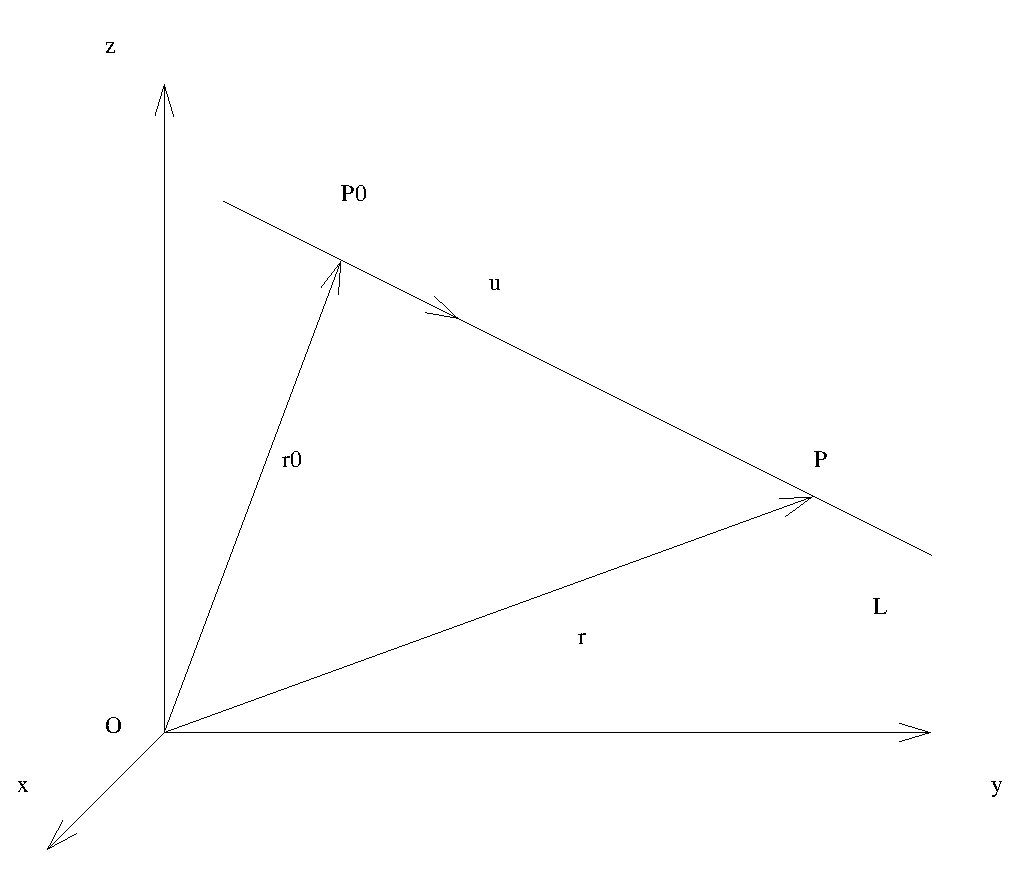
\includegraphics[height=2in]{../../modules/vectors/pictures/ok-line_point_direction_scalar.eps}
    \end{figure}
\end{columns}
\end{frame}

\begin{frame}
\uncover<1->{ $$\left\{ \begin{array}{ll}
           x & = x_0 + t u_1 \\
	   y & = y_0 + t u_2 \\
           z & = z_0 + t u_3
          \end{array}
\right. \Longrightarrow \boxed{\frac{x-x_0}{u_1} = \frac{y-y_0}{u_2} = \frac{z-z_0}{u_3}} \text{ \textcolor[rgb]{0.98,0.00,0.00}{Symmetric equations}}$$}

\uncover<2->{Caution! If $u_2=0$ (for example), then:
%
$$\frac{x-x_0}{u_1} = \frac{z-z_0}{u_3} \quad  \text{ and } \quad y=y_0 $$}

\uncover<3->{Example: Line with direction $\textbf{u} = \langle 4,5,6\rangle$ through $P_0(1,2,3)$:}
\begin{itemize}
 \item<4-> Parametric vectorial equation:
%
$$\textbf{r} = \langle 1,2,3\rangle + t \langle 4,5,6\rangle \leftrightarrow
\textbf{r} = \langle 1+4t, 2+5t, 3+6t\rangle$$
%
\item<5-> Parametric scalar equations:
%
$$\left\{ \begin{array}{ll}
           x & = 1 + 4t \\
	   y & = 2+5t \\
           z & = 3+6t
          \end{array}
\right. , \quad t \text{ real number.}$$
%
\item<6-> Symmetric equations:
%
$$\frac{x-1}{4} = \frac{y-2}{5} = \frac{z-3}{6}\; .$$
\end{itemize}

\end{frame}
\item \begin{frame}
 \frametitle{Line from Two Points}

\begin{columns}

\column{0.4\textwidth}
\psset{xunit=1.4cm, yunit=1.4cm}
\begin{pspicture}(-1,-0.4)(2,2.1)
\fcBoundingBox{-0.8}{-0.4}{4}{2.1}
\renewcommand{\fcScreen}{[-3 -1 -0.2] 0}
\tiny
\uncover<5->{\fcAxesIIId{2}{2}{2}}
\fcLineIIId{[0.5 0.5 1]}{[3 3 0.5]}
\fcLineIIId{[0.5 0.5 1]}{[4 4 0.3]}
\fcLineIIId[arrows=->]{[0 0 0]}{[1 1 0.9]}
\fcPutIIId[br]{[0.5 0.5 0.45]}{$\fcv r_0~$}

\fcLineIIId[linecolor=blue, arrows=->]{[1 1 0.9]}{[2.5 2.5 0.6]}
\fcPutIIId[br]{[1.75 1.75 0.8]}{$\fcv u$}

\fcLineIIId[arrows=->]{[0 0 0]}{[2.5 2.5 0.6]}
\fcPutIIId[b]{[1.25 1.25 0.3]}{$\fcv r_1$}

\fcDotIIId{[1 1 0.9]}
\fcPutIIId[lb]{[1 1 0.95]}{$P_0\uncover<5->{(x_0,y_0, z_0)} $}
\fcDotIIId{[2.5 2.5 0.6]}
\fcPutIIId[lb]{[2.5 2.5 0.65]}{$P_1\uncover<5->{(x_1, y_1, z_1)}$}
\fcDotIIId{[3.5 3.5 0.4]}
\fcLineIIId[arrows=->]{[0 0 0]}{[3.5 3.5 0.4]}
\fcPutIIId[b]{[1.75 1.75 0.2]}{$\fcv r$}
\fcPutIIId[b]{[3.5 3.5 0.5]}{$~P(x,y,z)$}
\fcPutIIId[t]{[4 4 0.3]}{$~L$}
\fcPutIIId[r]{[0 0 0.1]}{$O~~$}
\end{pspicture}
\column{0.6\textwidth}
\begin{itemize}
\item Given: distinct points $P_0$ and $P_1$, position vectors $\textbf{r}_0$ and $\textbf{r}_1$.
\item Goal: write equations of line $L$ through $P_0$ and $P_1$.
\item<2-> Direction of $L$: $\textbf{u} = \textbf{r}_1 - \textbf{r}_0$.
\item<5-> $\fcv{u} = \langle x_1-x_0,y_1-y_0,z_1-z_0\rangle$
\end{itemize}. 
\end{columns}
\uncover<3->{
\begin{definition}
\alert<1->{Parametric vectorial equation} of a line $L$:\\
$
\textbf{r} = \textbf{r}_0 + t(\textbf{r}_1-\textbf{r}_0)
\quad \Leftrightarrow \quad   \textbf{r} = (1-t)\textbf{r}_0 + t\textbf{r}_1
$

\uncover<5->{
\alert<1->{Parametric scalar equations} of a line $L$:
$\left|
\begin{array}{ll}
x & = x_0 + t(x_1-x_0) \\
y & = y_0 + t(y_1-y_0) \\
z & = z_0 + t(z_1-z_0)
\end{array}
\right. \Leftrightarrow \left| \begin{array}{ll}
x & = (1-t)x_0 + tx_1 \\
y & = (1-t)y_0 + ty_1 \\
z & = (1-t)z_0 + tz_1
\end{array}
\right. , \quad t \text{ real number.}$
} %uncover
\end{definition}
} %uncover
\end{frame}
\item \label{problemEquationsAllDiagonalsCubeContainingOrigin}
We recall that the 8 points $(1,1,1), (-1,1,1), (1,-1,1), (-1,-1,1), (1,1,-1)$, $(-1,1,-1), (1,-1,-1), (-1,-1,-1)$ (all possible sign combinations) give the vertices of a cube with edge 2 units.
 
Find equations for all lines connecting two vertices in the cube above that pass through the origin (how many connecting two vertices of a cube are there? How many of them are edges?).


\answer{ There are $4$ such edges. See the solution below for their equations.
}
\solution{\ref{problemEquationsAllDiagonalsCubeContainingOrigin}.
A cube has a total of $8 $ vertices. A line is given by two (distinct) points, therefore there are $\binom {8}{2}= \frac{8\cdot 7}{2}= 28$ total lines connecting two distinct vertices of a cube. Of those $12$ lines are cube edges, $12 = 6\cdot 2$ are diagonals of cube faces, and $4 $ are inner diagonals. All four inner diagonals contain the origin. A justification for this can undoubtedly be given by writing all $28$ line equations. However, the origin is in the center of the cube, and we know from our every-day geometric intuition that only the inner diagonals contain the center of a cube; we give no further justification.

The $4$ inner diagonals of the cube, call them $L_1, L_2, L_3, L_4$ pass through the points 

$\begin{array}{rcl}
(1,1,1), (-1,-1,-1) &\in& L_1\\
(1,1,-1), (-1,-1,1) &\in& L_2\\
(1,-1,1), (-1,1,-1) &\in& L_3\\
(-1,1,1), (1,-1,-1) &\in& L_4
\end{array}.
$

Therefore equations for these lines are given by:
$
\begin{array}{rl}
L_1:&  t\langle 1, 1, 1 \rangle\\
L_2:&  t\langle 1, 1, -1 \rangle\\
L_3:&  t\langle 1, -1, 1 \rangle\\
L_3:&  t\langle -1, 1, 1 \rangle\\
\end{array}
$.
}
\item Find an equation of the plane passing through the given point and with the given normal. Find parametric vectorial equations of the plane.

\begin{enumerate}
\item $P_0(2,3,5) $,  $\fcv n= \langle-3, -5, -7 \rangle$.
\item $P_0(1, 1, 1)$, $\fcv n= \langle 1,1,1 \rangle$.
\end{enumerate}
\solution{\ref{problemFindPlaneFromP(1,2,3)andn(4,5,6)}
As studied, an equation passing through $(1,2,3)$ and with normal $(4,5,6)$ has equation:

\[
\begin{array}{rcl}
\langle x, y, z\rangle\cdot \langle 4,5,6\rangle&=& \langle4,5,6\rangle\cdot \langle 1,2,3\rangle\\
4x +5y+6z&=&23
\end{array}
\]
To find parametric equations of the plane, we need to find two directions, $\fcv u, \fcv v$, that can be added to the base point to obtain all points in the plane. This means that a direction vector $\fcv u$ has to be perpendicular to $\fcv n$. Equivalently, a direction vector $\fcv u$ lies in the plane passing through the origin and orthogonal to $\fcv n$. This means $\fcv u\langle u_1, u_2, u_3\rangle$ satisfies the equation:
\begin{equation}\label{eqproblemFindPlaneFromP(1,2,3)andn(4,5,6)eq1}
\begin{array}{rcl}
\fcv u\cdot \fcv n&=&0\\
4 u_1+5u_2+6u_3&=&0.
\end{array}
\end{equation}
There are infinitely many solutions to that equation - in fact, for each point in the plane passing through the origin and orthogonal to $\fcv n$ there is one solution. However, we only need to find two such non-colinear solutions, and declare them to be our vectors $\fcv u$ and $\fcv v$. It is very easy to do that: if we set $u_1$ and $u_2$ to be arbitrary, then $u_3$ can always be chosen so as to make the equation above hold. There are a number of accepted ways to choose $u_1$ and $u_2$ in a not-so-arbitrary fashion. For reasons outside of the scope of this homework, such ways to choose $u_1$ and $u_2$ may be preferable to the choosing at random. Our scheme for choosing a vector $\fcv u$ will be to choose $u_1=1$ and $u_2=0$ (or the other way round for $\fcv v$), and then to rescale the resulting vector so all coordinates are integers and the first non-zero coordinate is positive. In other words, we select $\fcv u$ to be proportional to $\langle 1, 0, -\frac{4}{6} \rangle$, and $\fcv v$ to be proportional to $\langle 0, 1 ,-\frac{5}{6} \rangle$, i.e., we select
\[
\begin{array}{rcl}
\fcv u&=& \langle 3,0, -2 \rangle \\
\fcv v&=& \langle 0, 6, -5 \rangle
\end{array}. 
\] 
Finally we get that a parametric equation of the plane is given by:
\begin{equation}\label{eqproblemFindPlaneFromP(1,2,3)andn(4,5,6)eq2}
\langle 1,2,3 \rangle + s\langle 3,0, -2 \rangle +t\langle 0, 6, -5 \rangle\quad .
\end{equation}
The above equations are not unique; therefore our problem has many correct answers. 

A question arises: what do we need to do in order to check if two plane parametrizations are equivalent? Equivalently, how do we check that equation \eqref{eqproblemFindPlaneFromP(1,2,3)andn(4,5,6)eq2} gives a plane that coincides with the plane in given in \eqref{eqproblemFindPlaneFromP(1,2,3)andn(4,5,6)eq1}? Here's what we need to do to make sure our answer is correct (we leave the justification for that to the reader):
\begin{itemize}
\item Check that our $\fcv u, \fcv v$ are orthogonal to $\fcv n$. 
\item Check that our $\fcv u, \fcv v$ are not proportional to one another. 
\item Check that the base point of our equation is in the original plane. 
\end{itemize}

}
\item  Find an equation of plane $\mathcal P$ passing through the point and parallel to the given directions.

\begin{enumerate}
\item $P_0(1,2,3)$, $\fcv u=(2,3,5)$, $\fcv v=(3,5,7 )$.

\answer{$\mathcal P: z+y-4 x-1 =0$}
\item $P_0(1,1,1)$, $\fcv u=(1,-1,0)$, $\fcv v= (0,1,-1)$.
\answer{$\mathcal P:  z+y+x-3  =0$}
\end{enumerate}

\item \begin{frame}
 \frametitle{Plane from Three Points}

\begin{columns}
\column{0.4\textwidth}
\psset{xunit=0.8cm, yunit=0.8cm}
\begin{pspicture}(-0.2, -0.2)(3,3)
\tiny
\renewcommand{\fcScreen}{[-2 -1 -0.5] 0}
\fcParallelogramIIId{[-0.8 -0.8 3.6]}{[-1.4 2.4 1]}{[2.4 -1.4 1]}
\fcPutIIId[l]{[0 0 0.05]}{$~~O$}
\fcDotIIId{[0 0 0]}

\fcLineIIId[arrows=->, linestyle=dotted]{[0 0 0]}{[2 0 0]}
%\fcPutIIId{[1 0 0]}{$\fcv r_2$}
\fcLineIIId[arrows=->, linestyle=dotted]{[0 0 0]}{[0 2 0]}
%\fcPutIIId{[0 1 0]}{$\fcv r_0$}
\fcLineIIId[arrows=->, linestyle=dotted]{[0 0 0]}{[0 -0.4 2.4]}
%\fcPutIIId{[0 -0.2 1.2]}{$\fcv r_1$}
\fcDotIIId{[2 0 0]}
\fcDotIIId{[0 2 0]}
\fcDotIIId{[0 -0.4 2.4]}
\fcPutIIId[r]{[2 0 0]}{ $P_2(\fcv r_2)~$}
\fcPutIIId[tl]{[0 2 0]}{ $P_0(\fcv r_0)$}
\fcPutIIId[b]{[0 -0.4 2.4]}{ $P_1(\fcv r_1)$}
\fcLineIIId[arrows=->]{[0 2 0]}{[2 0 0]}
\fcPutIIId[t]{[1 1 -0.1]}{$~\fcv v$}
\fcLineIIId[arrows=->]{[0 2 0]}{[0 -0.4 2.4]}
\fcPutIIId[b]{[0 0.8 1.3]}{$~\fcv u$}%
\fcPerpendicularIIId{[4.8 6.8 4.8]}{ [0 2 0] [2 0 0]}{0.6}%
\fcPerpendicularIIId[arrows=<-]{[4.8 6.8 4.8]}{[0 2 0] [0 -0.4 2.4]}{0.6}%
\fcLineIIId[linestyle=dotted]{[0 0 0]}{[1.4 -0.84 1.44]}%
\fcPerpendicularIIId[arrows=<-]{[4.8 6.8 4.8]}{[0 2 0] [1.4 -0.84 1.44]}{0.8}%
\fcLineIIId[arrows=->]{[0 2 0]}{[1.4 -0.84 1.44]}%
\fcPutIIId[b]{[1.4 -0.84 1.44]}{$P(\fcv r)$}%
\end{pspicture}

\column{0.6\textwidth}
\begin{itemize}
\item Given: three non-collinear points $P_0(\fcv{r}_0)$, $P_1(\fcv{r}_1)$, $P_2(\fcv{r}_2)$.
\item Goal: find equations fo plane $\mathcal{P}$ passing through $P_0$, $P_1$, and $P_2$.
\item<2-> The plane is parallel to $\fcv{u} = \fcv{P}_0\fcv{P}_1 = \fcv{r}_1 -\fcv{r}_0$ and passing through $P_0$ $\Rightarrow$ this problem was solved previously.

\end{itemize}
\end{columns}
\only<3>{
Normal $\fcv{n} = \fcv{u} \times \fcv{v} =
(\fcv{r}_1-\fcv{r}_0) \times (\fcv{r}_2-\fcv{r}_0)$  \\

\alert<1->{Implicit equation}:
$$(\fcv{r}-\fcv{r}_0) \cdot \fcv{n} = 0$$
$$\boxed{(\fcv{r}-\fcv{r}_0) \cdot [(\fcv{r}_1-\fcv{r}_0) \times (\fcv{r}_2-\fcv{r}_0)] = 0}$$
$$\text{Vol}(R(\fcv{P}_0\fcv{P}, \fcv{P}_0\fcv{P}_1, \fcv{P}_0\fcv{P}_2)) = 0$$
}

\only<4>{
\alert<1->{Implicit equation}: $(\fcv{r}-\fcv{r}_0) \cdot [(\fcv{r}_1-\fcv{r}_0) \times (\fcv{r}_2-\fcv{r}_0)] = 0$

Let the points have coordinates $P_0(x_0,y_0,z_0)$, $P_1(x_1,y_1,z_1)$, $P_2(x_2,y_2,z_2)$. $P(x,y,z)$ is on plane $\mathcal{P}$:

\alert<1->{Implicit scalar equation}:
$\left| \begin{array}{ccc}
x-x_0 & y-y_0 & z-z_0 \\
x_1-x_0 & y_1-y_0 & z_1-z_0 \\
x_2-x_0 & y_2-y_0 & z_2-z_0
\end{array}
\right| = 0\; .$
}

\vskip 10cm
\end{frame}



\item Find the distance between the line and the point.

\begin{enumerate}
\item The line passing through $P_0(1,1,1)$ and $P_1(-1,-1,-1)$ and the point $Q(1,0,0)$.
\answer{$\frac{\sqrt{6}}{3} $}
\item The line passing through $P_0(-2,3,-5)$ and $P_1(3,4,5)$ and the point $Q(2,-2,2)$. 
\answer{$\frac{\sqrt{57610}}{42}$}
\end{enumerate}



\item Find the distance between the plane and the point.

\begin{enumerate}
\item The plane passing through $P_0(1,2,3) $, $P_1(2,3,5)$ and $P_2(3,5,7)$ and the point $Q(2,-2,2)$.
\answer{$\frac{3}{5}\sqrt{5}$}
\item The plane passing through $P_0(1,2,3) $, $P_1(2,3,5)$ and $P_2(3,5,7)$ and the point $Q(5,7,11)$.
\answer{$0$}
\item The plane passing through the points $P_0(1,1,1)$, $P_1(1,-1,-1)$, $P_2(-1,-1,1)$ and the point $Q(-1,1,-1)$.
\answer{$\frac{4}{3}\sqrt{3}$}
\end{enumerate}

\begin{comment}
Calculator code to solve above problem:

p0:=(1,2,3); 
p1:=(2,3,5);
p2:=(3,5,7);
q:=(2,-2,2);
u1:=p1-p0;
u2:=p2-p0;
u:=q-p0;
n:=u1\times u2;
((u n^t)_1)_1 /\sqrt{}(((n n^t)_1)_1) 
\end{comment}

\item Recall that a regular tetrahedron can be realized using 4 vertices of a cube. 

Find the angle between two edges of a regular tetrahedron. 
\item Recall that a regular tetrahedron can be realized using 4 vertices of a cube. 

Find the distance between two opposite edges of a regular tetrahedron inscribed in a 2x2x2 cm cube.
\item \begin{frame}
\frametitle{Distance between non-parallel lines}
\begin{columns}
\column{0.4\textwidth}
\begin{pspicture}(-2, -2)(2,2)
\tiny
\renewcommand{\fcScreen}{[-1 0 -0.5] 0}
\fcBoundingBox{-2}{-2}{2}{2}
\uncover<2->{%
\fcParallelogramIIId{[1.2 -1.2 1]}{[1.2 1.2 1]}{[-1.2 -1.2 1]}
\fcPutIIId[b]{[-1.2 -1.2 1]}{$\mathcal P$}
}%
\fcLineIIId{[-1 -1 -1]}{[1 1 -1]}
\fcLineIIId{[1 -1 1]}{[-1 1 1]} 
%\fcPerpendicularIIId[arrows=->, linecolor=green]{[0 0 -1]}{[1 -1 1] [-1 1 1]}{0.2}
\fcPutIIId[l]{[-1 1 1]}{$~~L_1$}
\fcPutIIId[r]{[-1 -1 -1.2]}{$L_2$}
\uncover<6->{%
\fcLineIIId[linestyle=dotted]{[0 0 1.3]}{[0 0 -1.3]}%
\fcPutIIId[rt]{[-0.1 0.1 -1]}{$Q_2~~~$}%
}%
\uncover<10->{%
\fcPerpendicularIIId[linestyle=none]{[0 0 -0.125]}{[0 0 1] [1 1 1]}{0.2}%
\fcPerpendicularIIId[linestyle=none]{[0 0 -0.125]}{[0 0 1] [-1 1 1]}{0.2}%
}%
\uncover<13->{%
\fcLineIIId[arrows=->, linecolor=green]{[0.8 -0.8 1]}{[0.9 0.9 -1]}%
\fcLineIIId[arrows=->, linecolor=green]{[0 0 1]}{[0.1 1.7 -1]}%
\fcDotIIId{[0.1 1.7 -1]}%
\fcPutIIId[l]{[0.1 1.7 -1]}{$~~R$}%
\fcPutIIId[l]{[0.05 0.85 0]}{$\fcv r_2- \fcv r_1$}%
}%
\uncover<6->{%
\fcPerpendicularIIId{[0.8 0.8 -1]}{[0 0 -1]}{0.2}
}%
\uncover<14->{\fcLineIIId[arrows=->, linecolor=brown]{[0.8 -0.8 1]}{[0 0 1]}%
\fcLineIIId[arrows=->, linecolor=brown]{[0.9 0.9 -1]}{[0.1 1.7 -1]}%
}%
\uncover<15->{%
\fcPerpendicularIIId{[0.1 1.7 -1]}{[0 0 -1]}{0.2}%
}%
\uncover<11->{%
\fcLineIIId[arrows=->, linecolor=blue]{[0 0 1]}{[0 0 -0.125]}%
\fcPutIIId[r]{[0 0 0.4375]}{$\fcv n~$}
}%
\uncover<4->{%
\fcLineIIId[linestyle=dotted]{[-1 -1 1]}{[1 1 1]}
\fcPutIIId[l]{[1 1 1]}{$~~L_2'$}
}%
\fcLineIIId[linecolor=red, arrows=->]{[0 0 -1]}{[0.75 0.75 -1]}
\fcPutIIId[t]{[0.325 0.325 -1.1]}{$\fcv u_2$}
\fcDotIIId{[0 0 -1]}
\uncover<12->{%
\fcDotIIId{[0.8 -0.8 1]}%
\fcPutIIId[br]{[0.8 -0.8 1]}{$P_1~$}%
\fcDotIIId{[0.9 0.9 -1]}%
\fcPutIIId[tr]{[0.9 0.9 -1]}{$P_2~$}%
}%
\uncover<5->{%
\fcDotIIId{[0 0 1]}
\fcPutIIId[r]{[-0.1 0.1 1]}{$Q_1~~~$}
}%
\fcLineIIId[linecolor=red, arrows=->]{[0 0 1]}{[-0.75 0.75 1]}
\fcPutIIId[br]{[-0.325 0.325 1]}{$\fcv u_1$}
\uncover<2->{
\fcLineIIId[linecolor=red, arrows=->]{[0 0 1]}{[0.75 0.75 1]}
\fcPutIIId[t]{[0.325 0.325 0.9]}{$\fcv u_2$}
}
%\fcPutIIId{[2 2 0]}{%
%\fcLineIIId[linecolor=red, arrows=->]{[0 0 1]}{[-0.75 0.75 1]}
%\fcPutIIId[br]{[-0.325 0.325 1]}{$\fcv u_1$}
%\fcLineIIId[linecolor=red, arrows=->]{[0 0 1]}{[0.75 0.75 1]}
%\fcPutIIId[t]{[0.325 0.325 0.9]}{$\fcv u_2$}
%}%
\end{pspicture}

\column{0.6\textwidth}
\begin{itemize}
\item Given: lines $\begin{array}{rrcl}L_1: & \fcv{r}&=& \fcv{r}_1+t\fcv{u}_1 \\ L_2:& \fcv{r} &=& \fcv{r}_2+s\fcv{u}_2\end{array}$
\item The lines are skew or intersecting, i.e., $\fcv{n} = \fcv{u}_1 \times \fcv{u}_2 \neq \fcv{0}$.
\item Goal: find distance between the lines = $d(L_1, L_2)$ = shortest distance b-n points on the two lines.
\end{itemize}
\end{columns}
\begin{itemize} 
\only<handout:1|1-8>{
\item<2-> Construct plane $\mathcal P$ with directions $\fcv u_1$, $\fcv u_2$ and passing through $L_1$. 
\item<3-> Distance b-n $L_2$ and points on $\mathcal P$ is constant.
\item<4-> Project $L_2$ orthogonally on $\mathcal P$; let the projection be $L_2'$.
\item<5-> Let $L_2' $ and $L_1$ intersect in point $Q_1$.
\item<6-> Let $Q_2$ be the heel of the perpendicular from $Q_1$ onto $Q_2$.
\item<7-> $\Rightarrow$ $Q_1Q_2=d(L_1, L_2)$.
}
\only<handout:1|8-16>{
\item \alert<8,9>{$|Q_1Q_2|=d(L_1, L_2)$}.
}
\only<handout:2|9-16>{
\item<10-> $\fcv Q_1\fcv Q_2 \perp L_1, L_2$ \uncover<11->{$\Rightarrow$  $\fcv Q_1 \fcv Q_2$ is proportional to $\fcv n = \fcv u_1\times \fcv u_2$.}
\item<12-> Pick arbitrary points on $L_1, L_2$ - say, the base points $P_1(\fcv r_1), P_2(\fcv r_2)$.
\item<13-> Let $R$ be such that $\fcv Q_1\fcv R=\fcv P_1 \fcv P_2=\fcv r_2-\fcv r_1$. 
\item<14-> Then $\fcv{P}_2\fcv R$ is proportional to $\fcv u_1$.
\item<15-> $\Rightarrow $ $\fcv Q_2\fcv R= \fcv Q_2  \fcv P_2+\fcv{P}_2\fcv{R}$ is perpendicular to $\fcv n$.
}
\only<handout:3|16->{
\item<16->\alert<16,17>{ $\Rightarrow$ $\fcv Q_1 \fcv Q_2= \fcv {proj} _{\fcv n} (\fcv r_2-\fcv r_1)$.}
}
\only<handout:3|17->{
\item<18-> 
$d(L_1,L_2)  = |\fcv{proj}_{\alert<19>{\fcv{n}}} (\fcv{r}_2-\fcv{r}_1)| \uncover<19->{= \boxed{\frac{|(\fcv{r}_2-\fcv{r}_1)\cdot \alert<19,20>{\fcv{n}} | }{ |\alert<19,20>{\fcv{n}}|}}} \uncover<20->{= \frac{ |(\fcv{r}_2 -\fcv{r}_1 )\cdot (\alert<20>{ \fcv{u}_1\times \fcv{u}_2})|}{ | \alert<20>{\fcv{u}_1\times \fcv{u}_2}|}}$
\item<21-> If lines are intersecting we know $d(L_1,L_2)=0$. \uncover<22->{Since the lines intersect $L_2$ and $L_2'$ coincide.} \uncover<23->{$\Rightarrow$ $(\fcv{r}_2-\fcv{r}_1) \cdot (\fcv{u}_1\times \fcv{u}_2) = 0$} \uncover<24->{$\Rightarrow $ the formula $d(L_1, L_2)= \frac{|(\fcv{r}_2 - \fcv{r}_1 )\cdot (\fcv{u}_1\times \fcv{u}_2)|}{ | \fcv{u}_1\times \fcv{u}_2|}=0$ produces the expected result.}
}
\end{itemize}

\vskip 5cm
\end{frame}


\solution{\ref{problemDistanceLineLine(1,2,3)(6,5,4)to(1,3,5)(2,4,6)}
We need to first establish whether the two lines are parallel. Let $\fcv u$ be the direction vector of the first line given by
\[\fcv u=\fcv Q_0 \fcv Q_1= ( 6,5,4)-( 1,2,3) = (5,3,1)
\]
and let $\fcv v$ be the direction vector of the second line given by
\[
\fcv v=\fcv P_0 \fcv P_1= (2,4,6 )-(1,3,5)=( 1, 1, 1).
\]
Now it is straightforward to see that the two lines are not parallel - indeed, one immediately sees that $\fcv u= (5,3,1)$ is not a scalar multiple of $\fcv v=(1,1,1)$. Since the two lines are not parallel, the two direction vectors determine a plane through the origin whose normal vector is given by
\[
\fcv n= \fcv u\times \fcv v=  (5,3,1)\times ( 1, 1, 1)= \left| \begin{array}{ccc} \fcv i & \fcv j &\fcv k\\ 5&3&1 \\1 &1 &1\end{array}\right|= 2\fcv i -4\fcv j+ 2\fcv k= (2, -4, 2)\quad .
\]
We note that if the vectors $\fcv u, \fcv v$ were parallel, then the cross product above would had been zero. Now the distance between the two lines is obtained by taking an arbitrary vector with tail on one line and head on the other, and computing the length of its projection it onto $\fcv n $. We use the vector $\fcv r= \fcv Q_0\fcv P_0$. Then the distance $d$ between the two lines is given by:
\[
d=\frac{|\fcv r \cdot \fcv n| }{|\fcv n|}= \frac{|\left(( 1,3,5) - ( 1,2,3)\right) \cdot \fcv  n|}{|\fcv n|}=\frac{ |( 0, 1, 2 )\cdot( 2, -4,2 )|}{|\fcv n|}=0.
\]
Therefore the distance between the two lines is zero. This completes our solution.

We note that since the distance between the lines is zero, they must intersect. As a consistency check for our work, let us verify that the two lines do indeed intersect. The first line is parametrized by $( 1,2,3)+t( 5,3,1) $ i.e., has parametric equations

\[
\left|\begin{array}{rcl}x&=& 1 +5t \\y&=&2+3t\\z&=&3+t \end{array}\right.\quad .
\]
Similarly, the second line is given by the equations
\[
\left|\begin{array}{rcl}x&=& 1 +s \\y&=&3+s\\z&=&5+s \end{array}\right.\quad .
\]
Therefore to find an intersection of the two lines, we need to solve the system
\[
\left|\begin{array}{rcl} 1 +5t&=&1+s \\2+3t&=&3+s\\3+t&=&5+s \end{array}\right.\quad.
\]
From the first equality we get that $s=5t$. We substitute that into the second equality to get that $t=-\frac{1}{2}$. Therefore the intersection of the two lines is the point

\[
(1,2,3)-\frac{1}{2}(5,3,1)= \left(-\frac{3}{2}, \frac{1}{2}, \frac{5}2\right)= (1,3,5)-\frac{5}{2}(1,1,1)\quad ;
\]
all our error checks have been successful.
}

\solution{\ref{problemDistanceLineLine(1,3,4)(2,3,1)to(1,2,2)(0,2,5)}
We present a solution in a concise form suitable for exam taking.

Let $L_1, L_2$ be the two lines.
\[
\begin{array}{rcll|l}
\fcv u &=& (2,3,1)-(1,3,4)=(1,0,-3)&& \text{direction vector } L_1\\
\fcv v &=& (0,2,5)-(1,2,2)=(-1,0,3)=-\fcv u&&\text{direction vector } L_2\\
&&\text{Therefore } L_1 \parallel  L_2\\
\fcv r&=&(2,3,1)-(0,2,5)=(2,1,-4) &&\text{arbitrary vector connecting } L_1, L_2\\
L_1\parallel L_2\Rightarrow\\
\text{dist}(L_1,L_2)&=&|\fcv{orth}_{\fcv u} \fcv r| \\
&=&\left|\fcv r- \fcv {proj}_{\fcv u} \fcv r \right|\\
&=&\left|\fcv r- \frac{\fcv r \cdot \fcv u}{|\fcv u|^2}\fcv{u} \right|\\
&=&\left| (2,1,-4)-\frac{(2,1,-4)\cdot (1,0,-3)}{1^2+0^2+(-3)^2}(1,0,-3) \right|\\
&=&\left|\left(\frac{3}{5}, 1, \frac{1}{5} \right)\right|\\
&=&\sqrt{\left(\frac{3}{5}\right)^2+ 1^2+ \left(\frac{1}{5}\right)^2 }\\
&=&\frac{\sqrt{35}}{5} \quad .
\end{array}
\]
}

\solution{\ref{problemDistanceLineLine(1,3,4)(2,3,1)to(1,2,2)(0,2,4)}
We present a solution in a concise form suitable for exam taking.
\[\begin{array}{rcll|l}
\fcv u &=& (2,3,1)-(1,3,4)=(1,0,-3)&& \text{direction vector } L_1\\
\fcv v &=& (0,2,4)-(1,2,2)=(-1,0,2)=-\fcv u&&\text{direction vector } L_2\\
\fcv r &=& (1,3,4)-(1,2,2)=(0, 1, 2)  &&\text{arbitrary vector connecting } L_1,L_2\\
\fcv n&=&u\times v=(0, 1, 0) &&\neq 0\Rightarrow L_1\not \parallel L_2\\
L_1\not \parallel L_2\Rightarrow \\
\text{dist}(L_1,L_2)&=&\left|\fcv {proj}_{\fcv n} \fcv r\right|\\
&=&\left|\fcv r \cdot \frac{\fcv n}{|\fcv n|}\right|\\
&=&\left| (0,1,2)\cdot (0,1,0)\right|\\
&=&1\quad .
\end{array}
\]
}

\item Find the angle between the line and the plane.

\begin{itemize}
\item The line passing through $(-1,-1,-1) $ and $(1 , 1, 1)$ and the plane with equation $z=-1$.
\item The line passing through $(2,3, 5)$ and $(3,5,7)$ and the plane passing through $(1,0,0)$, $(0,1,0)$ and $(0,0,1)$.
\end{itemize}
\item Recall that a regular tetrahedron can be realized using 4 vertices of a cube. Find the angle between an edge of a regular tetrahedron and one of the two sides of the tetrahedron not containing the edge.
\item Recall that a regular tetrahedron can be realized using 4 vertices of a cube.

Find the angle between two faces of a regular tetrahedron.
}

\homeworkOnATopic{}{on Lecture 5 \\\standardHomeworkSubtitle}{5}{%
%DesiredHomeworkName: 
\item Find polar equations of the line given below.

\begin{enumerate}[ref={\fcProblemRef}]
\item The line $x+y=1$.
\answer{$\begin{array}{rcl} r(\cos \theta +\sin \theta)&=&1 \\ r=\frac{\sqrt{2}}{2}\sec \left(\theta -\frac{\pi}{4}\right) \end{array} $}
\item \label{problemWriteInPolarx+sqrt(3)y=2} The line $ x+\sqrt{3}y=2$.
\answer{ $\begin{array}{rcl} r\left(\frac{1}{2}\cos \theta +\frac{\sqrt{3}}{2}\sin \theta\right)&=& 1 \\ r=\sec \left(\theta-\frac{\pi}{3} \right) \end{array}$}
\item The line passing through $(3,5)$ and $(5,7)$.

\answer{$\begin{array}{rcl} x-y&=&-2\\ r(\cos \theta -\sin \theta)&=&-2\\ r=-\sqrt{2}\sec\left(\theta+\frac{\pi}{4} \right) \end{array} $}
\item The line passing through $(2,3)$ and $(-3,-2)$.
\answer{$\begin{array}{rcl} x-y&=&-1\\ r(\cos \theta -\sin \theta)&=&-1\\ r=-\frac{\sqrt{2}}{2} \sec \left( \theta + \frac{ \pi }{4} \right) \end{array} $}
\end{enumerate}
\item \solution{\ref{problemWriteInPolarx+sqrt(3)y=2}

Polar coordinates are given by
\[
\left|\begin{array}{rcl}
x&=& r\cos \theta\\
y&=& r\sin \theta 
\end{array}\right. .
\]
All we need to do to obtain polar equations for our line is substitute the above expressions in the equation for the line. 
\[
r\cos \theta + \sqrt{3}r\sin \theta= 2.
\]
This is a perfectly good answer, but we can transform the equation to make it look more compact:
\[
\begin{array}{rcll|l}
\displaystyle r\cos \theta + \sqrt{3}r\sin \theta&=&\displaystyle 2\\
\displaystyle r\underbrace{\frac{1}{2}}_{=\cos \left(\frac{\pi}{3}\right)} \cos\theta +r \underbrace{\frac{\sqrt{3}}{2}}_{=\sin \left(\frac{\pi}{3}\right)} \sin\theta &=&\displaystyle  1 \\
\displaystyle r\cos \left(- \frac{\pi }{3}\right)\cos \theta -\sin \left(- \frac{\pi }{3}\right)\sin \theta &=& 1&&   \text{use } \cos (a+b)= \cos a \cos b - \sin a \sin b\\
\displaystyle r\cos (\theta -\frac{\pi}{3})&=&1\\
r&=&\displaystyle \frac{1}{\cos \left(\theta - \frac{\pi}{3} \right)}\\
&=&\displaystyle \sec\left (\theta - \frac{\pi}{3}\right )\quad .

\end{array}
\]


}
\item Find polar equations of the circle given below.

\begin{enumerate}
\item The circle given by $(x-1)^2+y^2=1$.
\answer{$r=2\cos \theta$}
\item The circle given by $x^2+ x+y^2=1$.
\answer{$r^2+r\cos \alpha -1=0$}
\item The circle with center $(1,2)$ and radius $3$.
\answer{$r^{2} -4 r \sin{}\theta-2 r \cos{}\theta-4 =0$}
\item The circle with center $(2,3)$ and radius $4$.
\answer{$r^{2} -6 r \sin{}\theta-4 r \cos{}\theta-3 =0$}
\end{enumerate}
\item Find an equation of the plane in cylindrical coordinates.

\begin{enumerate}
\item The plane given by $x+y+z=1$.
\item The plane given by $2x+3y-5z=0$.
\item The plane passing through $(-1, 1, 1)$, $(1, 1, -1)$ and $(1, -1, 1)$.
\item The plane passing through $(2,3,5 )$, $(3, 5, 2)$ and $(5, 2, 3)$.
\end{enumerate}
\item Find an equation of the sphere in cylindrical coordinates.

\begin{enumerate}
\item The unit sphere.
\item The sphere with equation $x^2 +x+ y^2+2y + z^2 +3z=0$.
\item The sphere with center $(1,2,3)$ and radius $5$.
\end{enumerate}
\item Find an equation of the plane in spherical coordinates.

\begin{enumerate}
\item The plane given by $x+y+z=1$.
\item The plane given by $2x+3y-5z=0$.
\item The plane passing through $(-1, 1, 1)$, $(1, 1, -1)$ and $(1, -1, 1)$.
\item The plane passing through $(2,3,5 )$, $(3, 5, 2)$ and $(5, 2, 3)$.
\end{enumerate}
\item Find an equation of the sphere in spherical coordinates.

\begin{enumerate}
\item The unit sphere.
\item The sphere with equation $x^2 +x+ y^2+2y + z^2 +3z=0$.
\item The sphere with center $(1,2,3)$ and radius $5$.
\end{enumerate}
}

\homeworkOnATopic{}{on Lecture 6 \\\standardHomeworkSubtitle}{6}{%
%DesiredHomeworkName: 
\item
Compute the tangent vector, the normal vector and the curvature at each point on the curve.

\begin{enumerate}[ref={\fcProblemRef}]
\item The equator of the unit sphere $\fcv r(t)= ( \cos t, \sin t ,0 )$.
\item The equator of the unit sphere $\fcv r(t)= ( \cos t, \sin t ,0 )$.
\item The loxodromic curve $\fcv r(t)= ( \cos (10t) \sin (t), \sin (10t)\sin (t), \cos (t) )$. A loxodromic curve is a curve obtained by taking a straight line in the $\{(\rho,\phi, \theta)|\rho =\text{const}\}$-plane in spherical coordinates and mapping it into the $x,y,z$-coordinates. Loxodromic curves were used in navigation: maintaining a course on a loxodromic curve requires only keeping a constant angle with the north direction (which one approximately obtained via compass).

\begin{pspicture}(0,0)(1,1)
\fcCurveIIId[plotpoints=500, linecolor=red]{0}{180}{[10 t mul cos t sin mul 10 t mul sin t sin mul t cos ]}
\end{pspicture}
\item The ellipse $\fcv r(t) = ( a\cos t, b\sin t ) $. Where is the curvature largest? Where smallest? Can you answer without computation, and does your answer match your computation?
\item The loxodromic meridian
$\fcv r(t)=( \sin (at)\cos (bt),  \sin(at)\sin (bt) ,\rho\cos (at) )
$.
\item The trefoil (torus) knot
$\fcv r=( \left( R+r\sin \left(3t\right)\right) \cos (2t) ,(R+r\sin \left( 3t \right) \sin (2t) ,r\cos (3t))
$.
\item The torus curve
$\fcv r=( \left( R+r\sin \left(20t\right)\right) \cos (t) ,(R+r\sin \left( 20t \right) \sin (2t) ,r\cos (20t))
$.

\begin{pspicture}(0,0)(1,1)
\fcAxesIIId{3}{3}{2}

\pstVerb{
6 dict begin
/phi  {t 20 mul} def
/theta {t } def
/R 2 def
/r 0.2 def
/xyRad {phi sin r mul R add} def
/torusCurve {[theta cos xyRad mul theta sin xyRad mul phi cos r mul ]} def
}
\fcCurveIIId[linecolor=red, plotpoints=500]{0}{360 }{torusCurve}
\pstVerb{end}
\end{pspicture}
\item The helix $\fcv r= (\cos t, \sin t, t) $.

\item \label{problemComputeTangentNormalCurvature(tcost,tsint,-t)} The cone curve $\fcv r= ( t \cos t, t\sin t, -t) $.

\psset{xunit=0.3cm, yunit=0.3cm}
\begin{pspicture}(0,0)(1,1)
\fcCurveIIId[linecolor=red, plotpoints =500]{0}{720}{ [t cos t sin 1] t 57.295779513 div \fcVectorTimesScalar }
\end{pspicture}

\end{enumerate}

\item
Find the length of the curve.
\begin{enumerate}

\item The helix $\fcv r= (\cos t, \sin t, t) $, $t\in [0,2\pi]$.

\item The cone curve $\fcv r= t(\cos t, t\sin t, t) $, $t\in [0,2\pi]$.
\psset{xunit=0.3cm, yunit=0.3cm}
\begin{pspicture}(0,0)(1,1)
\fcCurveIIId[linecolor=red, plotpoints =500]{0}{360}{ [t cos t sin 1] t 57.295779513 div \fcVectorTimesScalar }
\end{pspicture}

\end{enumerate}

\item
Write down the integral expressing the length of the curve. Please do not try to solve the integrals by hand. Optionally, for this exercise only, you may type the integrals in an on-line computer algebra system and see what you get.

\begin{enumerate}
\item The loxodromic curve $\fcv r(t)= ( \cos (10t) \sin (t), \sin (10t)\sin (t), \cos (t) )$ from $t=0$ to $t=t_0$.
\item The ellipse $\fcv r(t) = ( a\cos t, b\sin t ) $ from $t=0$ to $t=t_0$.
\item The trefoil (torus) knot
$\fcv r=( \left( 3+\sin \left(3t\right)\right) \cos (2t) ,(3+\sin \left( 3t \right) \sin (2t) ,\cos (3t))
$
from $t=0$ to $t=2\pi$.
\item The torus curve
$\fcv r=( \left( R+r\sin \left(20t\right)\right) \cos (t) ,(R+r\sin \left( 20t \right) \sin (2t) ,r\cos (20t))
$
from $t=0$ to $t=2\pi$.
\end{enumerate}

}

\homeworkOnATopic{}{on Lecture 8 \\\standardHomeworkSubtitle}{8}{%
%DesiredHomeworkName: 
\item
Find the limit or show that it does not exist.

\begin{enumerate}
\item  \label{problem-lim-xytozero-(y^4)/(x^4+2y^2)} $\displaystyle \lim\limits_{(x,y)\to (0,0)}\frac{ y^4}{x^4+2y^2}$.

\answer{$0$}

\item $\displaystyle \lim\limits_{(x,y)\to (0,0)} \frac{x^2+\left(\ln (1+y)\right)^2}{x^2+y^2}$.

\answer{the limit does not exist.}

\item $\displaystyle \lim\limits_{(x,y)\to (0,0)} \frac{x^2\ln (1+y)}{x^2+y^2}$.

\answer{$0$}

\item $\displaystyle \lim\limits_{(x,y)\to (0,0)} \frac{x^2y^4}{x^4+y^8} .$

\answer{the limit does not exist.}

\end{enumerate}
\solution{
\ref{problem-lim-xytozero-(y^4)/(x^4+2y^2)}
Limits respect inequalities, therefore
\[
0\leq \lim\limits_{(x,y)\to 0} \frac{y^4}{x^4+2y^2}\leq \lim\limits_{(x,y)\to 0}\frac{y^4}{2y^2}= \lim\limits_{(x,y)\to 0}\frac{1}{2}y^2=0.
\]
Therefore $\lim\limits_{(x,y)\to 0} \frac{y^4}{x^4+2y^2}=0$.
}
}

\homeworkOnATopic{}{on Lecture 9 \\\standardHomeworkSubtitle}{9}{%
%DesiredHomeworkName: 
\item Compute the indicated partial derivatives. Answer key has not been proofread, use with caution.

\begin{enumerate}
\item $\frac{\partial r}{\partial x}$, $\frac{\partial r}{\partial y}$, $r=\sqrt{x^2+y^2}$.
\answer{$\frac{\partial r}{\partial x}=\frac{x}{ \sqrt{x^2+y^2}}= \frac{x}{r}$, $\frac{\partial r}{\partial y}=\frac{y}{\sqrt{x^2+y^2}} = \frac{y}{r}$}

\item $\frac{\partial^2 r}{\partial x^2}$, $\frac{\partial^2 r}{\partial y^2}$, $\frac{\partial^2 r}{\partial y\partial x}$, $r=\sqrt{x^2+y^2}$.
\answer{$\frac{\partial^2 r}{\partial x^2}= \frac{y^2}{r^3}$, $\frac{\partial^2 r}{\partial y^2}=\frac{x^2}{r^3} $, $\frac{\partial^2 r}{\partial y\partial x}=-\frac{xy}{r^2} $ }

\item \label{problemComputePartialDerivative-dtheta-dx-dy-arctan(y/x)} $\frac{\partial \theta}{\partial x}$, $\frac{\partial \theta}{\partial y}$, $\theta=\Arctan\left( \frac{y}{x} \right)$.
\answer{ $ \frac{\partial \theta}{\partial x}= \frac{-y}{x^2+y^2} $,  $ \frac{\partial \theta}{\partial y}= \frac{x}{x^2+y^2} $ }

\item $\frac{\partial^2 \theta}{\partial x^2}$, $\frac{\partial \theta^2}{\partial y\partial x}$, $\frac{\partial^2 \theta}{\partial y^2}$, $\theta=\Arctan\left( \frac{y}{x} \right)$.
\answer{Let $r=\sqrt{x^2+y^2}$. $\frac{\partial^2 \theta }{\partial x^2}= \frac{2xy}{(x^2+y^2)^2}$, $\frac{\partial^2 \theta }{\partial y^2}= \frac{-2xy}{(x^2+y^2)^2}$, $ \frac{\partial \theta^2}{\partial y\partial x} = \frac{y^2-x^2}{(x^2+y^2)^2}$ }
\end{enumerate}
\solution{\ref{problemComputePartialDerivative-dtheta-dx-dy-arctan(y/x)}

\[
\begin{array}{rcl}
\displaystyle\frac{\partial }{\partial x}\left(\Arctan\left(\frac{y}{x}\right) \right) &=&\displaystyle \frac{\frac{\partial }{\partial x} \left(\frac{ y}{ x} \right)}{ 1+\left(\frac{y}{x}\right)^2 }   = \frac{ -\frac{ y}{x^2}}{ 1+ \frac{ y^2 }{x^2}} = \frac{-y}{x^2+y^2}\\
\displaystyle\frac{ \partial }{\partial y}\left(\Arctan\left( \frac{y}{x} \right) \right)& =& \displaystyle \frac{\frac{\partial }{\partial y} \left(\frac{y }{x} \right) }{ 1 + \left( \frac{y}{x}\right)^2 }   = \frac{ \frac{ 1}{x }}{ 1+ \frac{ y^2 }{x^2 }} = \frac{ x }{ x^2+y^2}\\
\end{array}
\]
}
}

\homeworkOnATopic{}{on Lecture 10 \\ \standardHomeworkSubtitle}{10}{%
%DesiredHomeworkName: Directional_Derivatives_Variable_Changes_Differential_Operators
\item Recall that the directional derivative $D_{\fcv u}$ in the direction $\fcv u$ is defined as the covariant derivative  $D_{\fcv u}f= \nabla_{\frac{\fcv u}{|\fcv u|}} f$. Find the covariant derivative $\nabla_{\fcv u} f$ and the directional derivative $D_{\fcv u} f$ at the indicated point.

\begin{enumerate}[ref={\fcProblemRef}]
\item $f(x,y) = x^2+y^2$, $\fcv{u}= (1,2)$, $(x,y)=P=(2,1)$.

\answer{$\nabla_{\fcv u}f (P)= 8$, $ D_{\fcv u}f(P) = \frac{8}{5}\sqrt{5}  $}
\item $f(x,y) = e^{x+y}$, $\fcv{u}= (1,1)$, $(x,y)=P=(0,0)$.

\answer{$\nabla_{\fcv u}f (P)=2$, $ D_{\fcv u}f(P) =\sqrt{2}$}
\item $f(x,y, z) = \ln \sqrt{x^2+y^2+z^2}$, $\fcv{u}= (1,-1,1)$, $(x,y,z)=P=(1,1,1)$.

\answer{$\nabla_{\fcv u}f (P)= \frac{1}{3}$, $ D_{\fcv u}f(P) =\frac{\sqrt{3}}{9} $}
\item $f(x,y, z) = \ln \sqrt{x^2-2y^2+z^2}$, $\fcv{u}= (1,-1,2)$, $(x,y,z)=(1,1,2)$

\answer{$\nabla_{\fcv u}f (P)=\frac{7}{3}$, $ D_{\fcv u}f(P) =\frac{7}{18}\sqrt{6} $}
\item $f(x,y,z) = xyz$, $\fcv{u}= (-1,-2,3)$, $(x,y,z)=(1,1,1)$.

\answer{$\nabla_{\fcv u}f (P)=0$, $ D_{\fcv u}f(P)  =0$}
\end{enumerate}

\item \begin{enumerate}
\item Let the variables $b,c, x_1, x_2$ be related via $b=-x_1-x_2 $ and $c=x_1 x_2$.
\begin{enumerate}
\item Express the differential operators $\frac{\partial}{\partial c}$ and $\frac{\partial}{\partial b}$ via $\frac{\partial}{\partial x_1}$ and $\frac{\partial}{\partial x_2}$.
\item Express the differential operators  $\frac{\partial}{\partial x_1}$ and $\frac{\partial}{\partial x_2}$ via $\frac{\partial}{\partial c}$ and $\frac{\partial}{\partial b}$. 
\end{enumerate}

\item Let $x,y,z$ and $\rho, \phi,\theta$ be related via the usual spherical coordinates equations i.e., $x= $
\begin{enumerate}
\item \label{problemd/dx,d/dy,d/dzinspherical} Express the differential operators $\frac{\partial }{\partial x}, \frac{\partial }{\partial y}, \frac{\partial}{\partial z}$ via $\frac{\partial }{\partial \rho}$, $\frac{\partial }{\partial \phi}$, $\frac{\partial }{\partial \theta}$.

\answer{
$\begin{array}{rcl}
\frac{\partial}{\partial x} &=& \sin \phi \cos \theta \frac{\partial }{\partial \rho} +\frac{\cos \phi \cos \theta }{\rho} \frac{ \partial}{\partial \phi}-\frac{\sin \theta}{\rho\sin \phi} \frac{ \partial }{\partial \theta} \\ 
\frac{\partial}{\partial y}&=&\sin \phi \sin \theta \frac{\partial}{\partial \rho} + \frac{\cos \phi\sin\theta }{\rho} \frac{ \partial }{\partial \phi}+\frac{\cos\theta}{\rho\sin \phi} \frac{ \partial }{\partial \theta} \\ 
\frac{\partial}{\partial z}&=&\cos \phi  \frac{\partial}{\partial \rho} - \frac{\sin \phi}{\rho} \frac{ \partial }{\partial \phi}  
\end{array}$}
\item Express the differential operators $\frac{\partial }{\partial \rho}$, $\frac{\partial }{\partial \phi}$, $\frac{\partial }{\partial \theta}$ via $\frac{\partial }{\partial x}, \frac{\partial }{\partial y}, \frac{\partial}{\partial z}$.

\answer{ 
$\begin{array}{rcl}
\frac{\partial}{\partial \rho} &=& \frac{x}{\rho} \frac{\partial }{\partial x} +\frac{y}{\rho} \frac{ \partial}{\partial y}+\frac{z}{\rho} \frac{ \partial }{\partial z} =\frac{x}{\sqrt{x^2+y^2+z^2}} \frac{\partial }{\partial x} +\frac{y}{\sqrt{x^2+y^2+z^2}} \frac{ \partial}{\partial y}+\frac{z}{\sqrt{x^2+y^2+z^2}} \frac{ \partial }{\partial z}\\ 
\frac{\partial}{\partial \phi}&=&\frac{zx}{\sqrt{x^2+y^2}} \frac{\partial}{\partial x} + \frac{zy}{\sqrt{x^2+y^2}} \frac{ \partial }{\partial y}-\sqrt{x^2+y^2} \frac{ \partial }{\partial z} \\ 
\frac{\partial}{\partial \theta}&=&-y  \frac{\partial}{\partial x} + y \frac{ \partial }{\partial y}  
\end{array}$
}
\item \label{problemLaplaceInSpherical} Express the Laplace differential operator $\frac{\partial^2}{\partial x^2}+\frac{\partial^2}{\partial y^2}+\frac{\partial^2}{\partial z^2}$ via  $\frac{\partial }{\partial \rho}$, $\frac{\partial }{\partial \phi}$, $\frac{\partial }{\partial \theta}$ (in other words, write the 3 dimensional Laplace operator in spherical coordinates).

\answer{$\begin{array}{rcl}
\frac{\partial^2}{\partial x^2}&=&\\
\frac{\partial^2}{\partial y^2}&=&\\
\frac{\partial^2}{\partial z^2}&=&\\
\frac{\partial^2}{\partial x^2}+\frac{\partial^2}{\partial y^2}+ \frac{ \partial^2}{\partial z^2} &=&\\ 
\end{array}$}
\end{enumerate}
\end{enumerate}
\solution{\ref{problemd/dx,d/dy,d/dzinspherical}
\textbf{To be written.}

}
}

\homeworkOnATopic{}{on Lecture 11 \\\standardHomeworkSubtitle}{11}{%
%DesiredHomeworkName: Quadratic_Surfaces_Tangent_Planes
%\item Match the surface graph to its mathematical name and to its equation.

\begin{enumerate}
\item
\begin{pspicture}(-2,-2)
\renewcommand{\fcScreen}{[-2 -1 -0.9] 0}
\fcSurfaceDirectDraw{}{-1}{-1}{1}{1}{[u v u u mul v v mul add]}
\end{pspicture}

\end{enumerate}
\item Determine the type of the quadratic surface given by the equation.
\begin{enumerate}
\item 
$x^2 +y^2+z^2+x+2y+3z=0$.
\answer{sphere (also ellipsoid)}
\item $x^2 +2y^2+z^2+x+2y+3z=0$.
\answer{(circular) ellipsoid}
\item $x^2 +2y^2+3z^2+x+2y+3z=0$.
\answer{ellipsoid}
\item \label{problemTypeOfSurfacez^2+2y^2-3x^2+x+y+1=0} $z^2+2y^2-3x^2 + x+y+1=0 $.
\answer{(elliptic) hyperboloid one sheet}
\item $z^2-y^2+\frac{1}{4}x^2 + x-y+1=0 $.
\answer{(elliptic) hyperboloid two sheets}
\item $x^2+y^2-\frac{1}{4}z^2 + x-y+5=0 $.
\answer{(circular) hyperboloid one sheet}
\item $\frac{1}{4}x^2-y^2+z^2-x+1=0$
\answer{(elliptic) cone}
\item $-\frac{1}{4}x^2+y^2+z^2-x-1=0$
\answer{(circular) cone}
\item $xy +z^2+1=0$. Hint: write $x=\frac{1}{\sqrt{2}}(u+v)$, $y=\frac{1}{ \sqrt{ 2} } (u-v) $ for some new variables $u,v$. Solve the problem in the $z,u,v$ -coordinates. Argue that the (axes of the) $u,v,z$-coordinate system can be obtained from the $x,y,z$-coordinate system via rotation.
\answer{(circular) hyperboloid one sheet}
\item $x^2+2y^2+z=0 $.
\answer{(elliptic) paraboloid}
\item $x^2+y^2+2xy+z=0 $.
\answer{cylindrical paraboloid}
\item $x^2-y^2+2x+z=0 $.
\answer{parabolic hyperboloid}
\end{enumerate}
\solution{
\ref{problemTypeOfSurfacez^2+2y^2-3x^2+x+y+1=0}
We have that
\[
\begin{array}{rcl}
\displaystyle z^2+2y^2-3x^2 + x+y+1&=&0\\
\displaystyle z^2+ 2\left(y+\frac{1}{4}\right)^2 - 3\left(x-\frac{1}{6} \right)^2 -\frac{1}{8}+\frac{1}{12}+1&=&0\\
\displaystyle z^2+ 2\left(y+\frac{1}{4}\right)^2 &=&\displaystyle 3\left(x-\frac{1}{6} \right)^2-\frac{23}{24}
\end{array}
\]
This figure is given by sum of two squares equal to a square minus a positive number. That makes is a hyperboloid two sheet, as explained in the theoretical discussions.
\begin{pspicture}(-3, -3)(3,3)
\pstVerb{20 dict begin
/coeffZ 1 def
/coeffY 2 def
/coeffX 3 def
/xFun {v} def
/rightSide {xFun 1 6 div sub dup mul 3 mul 23 24 div sub} def
/xTipTop {23 24 div coeffX div sqrt 1 6 div add} def
/xTipBottom {23 24 div coeffX div sqrt -1 mul 1 6 div add} def
/yFun { u sin 1 4 div sub coeffY sqrt div  rightSide sqrt mul} def
/zFun { u cos coeffZ sqrt div  rightSide sqrt mul} def
}
\renewcommand{\fcScreen}{[-0.3 2 -0.75] -1\space}
\fcStartIIIdScene
\fcAxesIIIdFullInScene{-3}{-3}{-3}{3}{3}{3}
\fcSurfaceInScene[arrows=(none), iterationsV=4, iterationsU=18]{0}{3}{360}{xTipTop 0.004 add}{[xFun yFun zFun]}{}
\fcSurfaceInScene[arrows=(none), iterationsV=4, iterationsU=18]{0}{xTipBottom 0.004 sub}{360}{-3 1 3 div add}{[xFun yFun zFun]}{}
\fcFinishIIIdScene[true]
\fcPutIIId{[3.2 0 0]}{$x$}
\fcPutIIId{[0 3.2 0]}{$y$}
\fcPutIIId{[0 0 3.2]}{$z$}
\pstVerb{end}
\end{pspicture}
}
\item  Find an equation of the tangent plane to the surface at the given point. The surface is given via an implicit equation.

\begin{enumerate}[ref={\fcProblemRef}]
\item The sphere $x^2+y^2+z^2=1$ at $(x,y,z)=(\frac{\sqrt{3}}{3},\frac{\sqrt{3}}{3},\frac{\sqrt{3}}{3}) $.

\answer{ tangent plane: $x+y+z=\sqrt{3} $}

\item \label{problemTangentPlanex^2+y^2-z^2=-3at(2,3,4)} The two-sheet hyperboloid $x^2+y^2-z^2=-3$ at $(x,y,z)=(2,3,4) $.

\answer{ tangent plane: $2x+3y-4z=-3 $}

\item The ellipsoid $x^2+2y^2+3z^2=20 $ at $(x,y,z)=(3,2,1)$.

\answer{tangent plane: $3x+4y+3z=20$}
\end{enumerate}
\solution{\ref{problemTangentPlanex^2+y^2-z^2=-3at(2,3,4)}
As studied in the theory, the normal to the tangent plane to a surface given by implicit equation $f=0$ is given by $\nabla f$. Since the tangent plane passes through $(2,3,4)$, this determines the tangent plane. 
\[
\begin{array}{rcll|l}
f=x^2+y^2-z^2-3&=&0&&\text{Equation of the surface}\\
\nabla f&=& (2x,2y,-2z)\\
\nabla f_{|(x,y,z)=(2,3,4)}&=&(4, 6, -8)\\
\nabla f_{|(x,y,z)=(2,3,4)}\cdot (x-2,y-3,z-4)&=&0 &&\text{Equation of plane with normal }\\
4(x-2)+6(y-3)-8(z-4)&=&0\\
2x+3y-4z&=&-3 &&\text{Final answer in simplified form.}\\
\end{array}
\]
}
\item

Find the equation of the tangent plane to the graph of the function at the indicated point.
\begin{enumerate}
\item $z= x^2- y^2$, at the point $(1, 1,0)$.
\item $z= e^{-x^2-y^2}$, at the point $(0,0,1)$
\item $z= e^{x^2-y^2}$, at the point $(1,-1,1)$.
\item $z=\sqrt{3-x^2-y^2} $, at the point $(1,1,1)$.
\end{enumerate}
}

\homeworkOnATopic{}{on Lecture 12 \\\standardHomeworkSubtitle}{12}{%
%DesiredHomeworkName: Maxima_Minima_Lagrange_Multipliers
\item Using the second derivative test, find the local minima and maxima as well as the saddle points of the function. 


\begin{enumerate}
\item $f(x,y)= 1+x^3+y^3-3x y$.   

%\psset{xunit=0.4cm, yunit=0.4cm}
%\begin{pspicture}(-1, -1)(1,1)
%\tiny
%\renewcommand{\fcScreen}{[1 1.4 -1] 0}
%\fcStartIIIdScene
%\fcAxesIIIdInScene{5}{5}{5}
%\fcSurfaceInScene[arrows=none, colorUV=pink, linewidth=0.4]{-3}{-3}{4}{4}{[u v u 3 exp v 3 exp -3 u v mul mul 3 add add add]}{u 3 exp v 3 exp -3 u v mul mul 3 add add add dup 5 le exch -3 ge and}
%\fcFinishIIIdScene[fastsort=true]
%\end{pspicture}

\item $f(x,y)= x^3y+x^2-27y$.
\item $f(x,y)=e^{2y-x^2-y^2}$.
\item $f(x,y)=e^x\sin y$.
\item $f(x,y) =x^2+ y^2+ \frac{ 1}{ x^2y^2}$.
\end{enumerate}
\solution{
\ref{problemextremax^2+x^2y+y^3-2y}
The critical points of $f$ are given by:
\[
\begin{array}{rcl}
\frac{\partial f}{\partial x}=0&=&2 x y+2 x\\
\frac{\partial f}{\partial y}=0&=&3 y^{2}+x^{2}-4.
\end{array}
\]
The first equality implies $x(y+1)=0$, and we have two cases: $x=0$ and $y=-1$.

\noindent Case 1. $x=0$. We substitute in second equality and solve:
\[
\begin{array}{rcl}
3y^2-4&=&0\\
y^2&=&\displaystyle \frac{4}{3}\\
y&=&\displaystyle\pm 2\frac{\sqrt{3}}{3}.
\end{array}
\]
Case 1 provides us with two critical points, $(x,y)=\left(0, 2\frac{ \sqrt{ 3} }{3 }\right)$ and $(x,y)=\left(0,- 2\frac{\sqrt{3}}{3}\right)$.

\noindent Case 2. $x\neq 0$. It follows that $y=-1$. We substitute in the second equality and solve:
\[\begin{array}{rcl}
3+x^2-4&=&0\\
x^2&=&1\\
x&=&\pm 1\quad .
\end{array}
\]
Case 2 provides us with two additional critical points, $(x,y)=(1,-1)$ and $(x,y)=(-1,-1)$.

The Hessian matrix of $f$ and its determinant are:
\[
H=\left(\begin{array}{cc} 2 y+2& 2 x\\
2 x& 6 y \end{array}\right)\quad \det H=12y(y+1)-4x^{2}\quad .
\]
At $(x,y)=\left(0, 2\frac{ \sqrt{ 3} }{3 }\right)$, $\det H=  8 \sqrt{ 3} +16 >0$, and $\frac{\partial f}{\partial x^2} >0$ so $f$ has a local minimum at that point. At $(x,y)=\left(0, -2\frac{ \sqrt{ 3} }{3 }\right)$, we have $\det H=  - 8 \sqrt{3} +16 >0$. We further have $\frac{\partial f}{\partial x^2}= 2( \frac{ 2}{\sqrt{3}}-1)<0 $ so $f$ has a local maximum at that point. Finally at $(x,y)= (\pm 1,-1)$, we have $\det H=-4<0$ and so both points are saddle points of $f$.

Our final answer is as follows.
\begin{center}
\begin{tabular}{r|l}
$(x,y)$ & critical point type\\\hline
$\left(0 ,-2\frac{\sqrt{3}}{3}\right) $ &local maximum\\
$\left(0,2\frac{\sqrt{3}}{3}\right) $ &local minimum\\
$\left(-1,-1\right) $ & saddle\\
$\left(1,-1\right) $ &saddle
\end{tabular}
\end{center}
}
\item Find the maximum of the function subject to the given restriction, or show the maximum does not exist. 

The problems don't have an answer key yet. If you think that a problem is incorrectly posed, make a clean argument why that is the case. 
\begin{enumerate}[ref={\fcProblemRef}]
\item $f(x,y)=x^2+2 y^2$, $x y=1$.
\item $f(x,y)=4x+5y$, $x^2+y^2=13$.
\item $f(x,y)=x^2y$, $x^2+2y^2 =1$.
\item $f(x,y)=e^{x y}$, $x^3+y^3 =2$.
\item $f(x,y)=x+3y+5z$, $x^2+y^2+z^2 =35$.
\item $f(x,y)=x-z$, $x^2+3y^2+z^2 =1$.
\item $f(x,y)=xyz$, $x^2+3y^2+5z^2 =8$.
\item $f(x,y)=x^2y^2z^2$, $ x^2+y^2+z^2=1$.
\item $f(x,y)=x^2+y^2+z^2 $, $x^4+y^4+z^4 =1$.
\item $f(x,y)=x^4+y^4+z^4$, $x^2+y^2+z^2 =1$.
\item $f(x_1,\dots, x_n) = x_1+\dots +x_n$, $x_1^2+\dots +x_n^2 =1$.

\item \label{problemFindExtremay+xUnderRestrictiony^2+y+x^2+x=1} Find the local extrema of $f(x,y)=y+x$ when $x,y$ satisfy the restriction $y^2+y+x^2+x=1$.

\answer{
\begin{tabular}{r|l}
$(x,y)$ & critical point type\\\hline
$\left(\frac{-1-\sqrt{3}}{2},\frac{-1-\sqrt{3}}{2}\right) $ & minimum\\
$\left(\frac{-1+\sqrt{3}}{2} , \frac{ -1+\sqrt{3}}{2}\right)$ & maximum\\
\end{tabular}
}
\end{enumerate}
\solution{\ref{problemFindExtremay+xUnderRestrictiony^2+y+x^2+x=1}
The restriction is $g(x,y)= y^2+y+x^2+x-1=0$. We use the method of Lagrange multipliers. We have that $\nabla f= (1,1)$ and $\nabla g = \left(2y+1,2x+1 \right)$. We have a local extremum when $\lambda\nabla f= \nabla g$, i.e., when
\[
\begin{array}{rcl}
\lambda &=& (2y+1)\\
\lambda &=& (2x+1)\\
y^2+y+x^2+x-1&=&0
\end{array}
\]
The first two equations imply $y=x$. We substitute that into the last equation to get that $2x^2+2x-1=0$. The solutions to the latter are $x=  \frac{ -2\pm \sqrt{2^2-4\cdot 2\cdot(-1)}}{4}= \frac{-1\pm \sqrt{3}}{2}$. The only restriction on $(x,y)$ is that they lie on the curve $y^2 + y+ x^2 +x=1$ (a circle). A circle is a bounded and closed set in space. Therefore $f$ must attain both its minimum and its maximum on it. Therefore the two critical points are maximum and minimum of $f$. Substitution of our answer in $f$ shows that $f$ attains its minimum at $\left(x,y\right)=\left(\frac{-1-\sqrt{3}}{2},\frac{-1-\sqrt{3}}{2}\right)$ and its maximum at $\left(x,y\right)=\left(\frac{-1+\sqrt{3}}{2} , \frac{ -1+\sqrt{3}}{2}\right)$. Our final answer is below.

\begin{tabular}{r|l}
$(x,y)$ & max or min\\\hline
$\left(\frac{-1-\sqrt{3}}{2},\frac{-1-\sqrt{3}}{2}\right) $ & minimum\\
$\left(\frac{-1+\sqrt{3}}{2} , \frac{ -1+\sqrt{3}}{2}\right)$ & maximum\\
\end{tabular}
}
}

\homeworkOnATopic{}{on Lecture 13 \\\standardHomeworkSubtitle}{13}{%
%DesiredHomeworkName: Double_Integrals
\item Evaluate the double integral. The problems are taken from the double integrals section of your textbook, please use the answer key provided there.

\begin{enumerate}
\item $\displaystyle \iint\limits_{D} x^3y^2 \diff x \diff y $, $D=\{(x,y)| 0\leq x \leq 2, -x\leq y \leq x \}$.
\item $\displaystyle \iint\limits_{D} \frac{4y}{x^3+2}\diff x \diff y $, $D=\{(x,y)| 1\leq x\leq 2, 0 \leq y\leq 2x\}$.
\item $\displaystyle \iint\limits_{D}\frac{2y}{x^2+1} \diff x \diff y $, $D=\{(x,y)|0\leq x \leq 1, 0 \leq y \leq \sqrt{x} \}$.
\item $\displaystyle \iint\limits_{D}e^{y^2} \diff x \diff y $, $D=\{(x,y)|0\leq y \leq 1, 0\leq  x\leq y \}$.
\item $\displaystyle \iint\limits_{D} x\cos y \diff x \diff y $, $D$ bounded by $y=0$, $y=x^2$, $x=1$.
\item $\displaystyle \iint\limits_{D} (x+y)\diff x \diff y $, $D$ bounded by $y=\sqrt{x}$ and $y=x^2$.
\item $\displaystyle \iint\limits_{D}y^3 \diff x \diff y $, $D$ - triangle with vertices $(0,2), (1,1), (3,2)$.
\item $\displaystyle \iint\limits_{D} xy^2 \diff x \diff y $, $D$ enclosed by $x=0$ and $x^2+y^2=1$.
\item $\displaystyle \iint\limits_{D} (2x-y)\diff x \diff y $, $D$ bounded by circle with radius 2 centered at the origin.
\item $\displaystyle \iint\limits_{D} 2xy\diff x \diff y $, $D$- triangular region with vertices $(0,0), (1,2), (0,3)$.
\end{enumerate}
\item Evaluate the double integral. The answer key has not been proofread, use with caution.

\begin{enumerate}[ref={\fcProblemRef}]
\item \label{problemintegralxydxdyoverx=3,x+1=y^2,x=y^2+2y+3} $\iint_{\mathcal R} xy \diff x\diff y$ where $\mathcal R$ is bounded by the curves $x=3 $, $x+1=y^2$, $x= y^2+2y+3$.

\answer{$\frac{52}{15}$}
\item \label{problemintegralxydxdyovery=x^2+1,y=2x^2-x-1} 
$\iint_{\mathcal R} xy\diff x\diff y\quad .$

where $\mathcal R$ is the region enclosed by $y=x^2+1$ and $y=2x^2-x-1$.  

\end{enumerate}



\solution{\ref{problemintegralxydxdyoverx=3,x+1=y^2,x=y^2+2y+3}

\begin{pspicture}(-1.5, -3)(6,3)
\fcLabels{6}{3}
\pscustom*[linecolor=\fcColorAreaUnderGraph]{
\parametricplot{-2}{0}{t t mul 2 t mul add 3 add t }
\psline(3, 0)(3,2)
\parametricplot{2}{-2}{t t mul 1 sub t }
}
\pscustom*[linecolor=green]{
\psline(3, 0)(3,2)
\parametricplot{2}{0}{t t mul 1 sub t }
\psline(-1,0)(3,0)
}
\parametricplot[linecolor=\fcColorGraph]{-2.4}{2.4}{t t mul 1 sub t }
\rput[l](0.3, -2){$x= y^2-1$}
\parametricplot[linecolor=\fcColorGraph]{-2.661325}{0.661325}{t t mul 2 t mul add 3 add t }
\rput[lb](4, -2){$x= y^2+2y+3$}
\psline[linecolor=\fcColorGraph](3, -2.3)(3,3)
\rput[r](3, 2.9){$x= 3~$}
\fcFullDot{3}{-2}
\fcFullDot{3}{2}
\fcFullDot{3}{0}
\psline[linecolor=black, arrows=<->](-0.75,0.5)(3, 0.5)
\fcFullDot[linecolor=black]{-0.75}{0.5}
\fcFullDot[linecolor=black]{3}{0.5}
\rput[b](-0.75, 1.5 ){$(y^2-1,y)$}
\psline[linestyle=dotted, arrows=->](-0.75, 1.5)(-0.75, 0.5)
\rput[bl](3, 0.7 ){$~(3,y)$}
\rput(2, 1){$Q_1$}
\rput(1.5, -1){$Q_2$}
\fcAxesStandardNoFrame{-1.5}{-3}{6}{3}
\end{pspicture}

We start by plotting the region. $ x=y^2-1$ is a parabola symmetric across the $x$ axis; $x=y^2+2y+3$ is a parabola with vertex at $x=3$, $y=-2$. The two parabolas intersect when 
\[
\begin{array}{rcl}
x=y^2-1&=& y^2+2y+3\\
2y+4&=&0\\
y&=&-2\\
x&=&y^2-1=(-2)^2-1=3,
\end{array}
\]
i.e., when $(x,y)=(3, -2)$. The line $x=3$ intersects $x+1=y^2$ when $y^2= 3+1 = 4$, i.e., when $(x,y)=(3,\pm 2)$. The line $x=3$ intersects $x=y^2+2y+3$ when $3= y^2+2y+3$. This implies $y(y-2)=0$ and finally we conclude the intersections of $x=3$ with $x=y^2+2y+3$ are $(x,y)=(3,0)$ and $(x,y)= (3,2)$. We can conclude that there three curves are plotted as indicated in the figure. Of the 8 regions bounded by the curves only two are bounded, and only one of them is bounded by all three curves. Since no further instruction is given in the problem, we assume that the intended region is the one bounded by all three curves, i.e., the region indicated in the figure above (the other bounded region can be enclosed using two of the curves only). Let $Q_1$ and $Q_2$ be the regions indicated in the figure above. Those two regions are curvilinear trapezoids with vertical bases. Consider the region $ Q_1$. Fix the $y$ coordinate of a point in $Q_1$. The figure shows that, for that fixed value of $y$, $x$ varies between $y^2-1$ and $3$. For $Q_2$, it similarly follows that, for a fixed $y$, $x$ varies between $y^2-1$ and $y^2+2y+3$. The points in $Q_1$ have $y$ coordinates in the range $y\in [ 0 , 2 ] $, and similarly, in $Q_2$ we have that the $y$ coordinate varies in the range $y\in [ -2 , 0 ] $. Thus our regions are parametrized as
\[
\begin{array}{rcl}
Q_1&=&\{(x,y)| 0\leq y\leq 2, y^2-1\leq x\leq 3 \}\\
Q_1&=&\{(x,y)| -2\leq y\leq 0, y^2-1\leq x\leq y^2+2y+3 \}.\\
\end{array}
\]

Finally our integral becomes 
\[
\begin{array}{rcl}
\displaystyle \iint_{\mathcal R} xy\diff x \diff y&=&\displaystyle \iint_{Q_1}xy \diff x \diff y + \iint_{Q_2}\diff x\diff y \\
&=&\displaystyle \int_{y=0}^{y=2} \left(\int_{x=y^2-1}^{x=3} xy \diff x\right) \diff y+ \int_{y=-2}^{y=0} \left( \int_{x=y^2-1}^{x=y^2+2y+3} xy \diff x \right) \diff y\\
&=&\displaystyle \int_{y=0}^{y=2}\left[ \frac{x^2y}{2}\right]_{x=y^2-1}^{x=3}\diff y+ \int_{y=0}^{y=3}\left[ \frac{x^2y}{2}\right]_{x=y^2-1}^{x=y^2+2y+3}\diff y\\
&=&\displaystyle \int_{y=-2}^{y=0}  \left(-\frac{1}{2} y (y^{2}-1)^{2}+\frac{9}{2} y \right)\diff y  +\int_{y=-2}^{y=0}\left( \frac{1}{2} y (y^{2}+2 y+3)^{2}-\frac{1}{2} y (y^{2}-1)^{2}\right)\diff y\\
&=&\displaystyle\int_{y=0}^{y=2}  \left(-\frac{1}{2} y^{5}+y^{3}+4 y  \right)\diff y  +\int_{y=-2}^{y=0}\left( 2 y^{4}+6 y^{3}+6 y^{2}+4 y\right)\diff y\\
&=&\displaystyle \left[-\frac{1}{12} y^{6}+\frac{1}{4} y^{4}+2 y^{2}\right]_{0}^{2} +\left[\frac{2}{5} y^{5}+\frac{3}{2} y^{4}+2 y^{3}+2 y^{2} \right]_{y=-2}^{y=0}\\
&=&\displaystyle \frac{20}{3} -\frac{16}{5} =\frac{52}{15}
\end{array}
\]

}
\item Integrate.

\begin{enumerate}
\item  \label{problemint_(y=0)^(y=sqrt(pi))int_(x=0)^(x=y)cos x^2 dx dy} $\displaystyle \int_{ y=0}^{ y=\sqrt{\pi}} \int_{x=y}^{x=\sqrt{\pi}} \cos \left( x^2 \right) \diff x\diff y$.
\end{enumerate}
\solution{\ref{problemint_(y=0)^(y=sqrt(pi))int_(x=0)^(x=y)cos x^2 dx dy}
The issue with this integral is that we cannot integrate  $\cos \left( x^2 \right)$ with respect to $x$ using (finitely many) elementary functions and their compositions. However, this expression is easy to integrate with respect to $y$. Therefore changing the order of integration (using Fubini's Theorem) could possibly help. Let the region of integration be $\mathcal R$. Then 
\[
\mathcal R=\left\{(x,y)| 0\leq y \leq \sqrt{\pi}, y\leq x \leq \sqrt{\pi} \right\}.
\]
We plot the region to find it is the triangle indicated in the figure below. When we fix the value of $x$, $y$ varies between $0$ and $x$. Therefore we can re-parametrize $\mathcal R$ via vertical slices:

\[\mathcal R=\left \{ (x,y)| 0\leq x\leq \sqrt{\pi}, 0\leq y\leq x \right \}. \]

\begin{pspicture}(-0.2,-0.2)(2,3)
\pscustom*[linecolor=\fcColorAreaUnderGraph]{%
\psline(0,0)(! 3.141592654 sqrt 0)(! 3.141592654 sqrt 3.141592654 sqrt)(0,0)
}%
\rput(1.3, 0.5 ){$\mathcal R$}
\fcAxesStandardNoFrame{-0.4}{-0.4}{2}{3}
\psline[linecolor=\fcColorGraph](0,0)(! 3.141592654 sqrt 0)(! 3.141592654 sqrt 3.141592654 sqrt)(0,0)
\psline[linecolor=black, arrows=<->](1,1)(1, 0)
\fcFullDot[linecolor=black]{1}{1}
\fcFullDot[linecolor=black]{1}{0}
\end{pspicture}
By Fubini's theorem, the iterated integral equals the double integral, which in turn can be evaluated using the iterated integral using the second parametrization of $\mathcal R$.
\[
\begin{array}{rcll|l}
\displaystyle \int_{ y=0}^{ y=\sqrt{\pi}} \int_{x=y}^{x=\sqrt{\pi}} \cos \left( x^2 \right) \diff x\diff y&=&\displaystyle  \iint_{\mathcal R} \cos \left(x^2\right)\diff x \diff y&&\text{By Fubini's Theorem}\\
&=& \displaystyle  \int_{x=0}^{\sqrt{\pi}}\int_{y=0}^{y=x}\cos \left(x^2\right)\diff y \diff x  &&\text{again by Fubini's Theorem}\\ 
&=&\displaystyle \int_{x=0}^{\sqrt{\pi}}\left[y\cos \left( x^2 \right) \right]_{ y=0}^{y=x}\diff x\\
&=&\displaystyle \int_{x=0}^{\sqrt{\pi}}x\cos \left(x^2\right)\diff x\\
&=&\displaystyle \int_{x=0}^{\sqrt{\pi}}\cos \left(x^2\right)\frac{1}{2} \diff \left(x^2\right)\\
&=&\displaystyle \frac{1}{2}\left[\sin \left(x^2\right)\right]_{x=0}^{x= \sqrt{ \pi}}\\
&=&\displaystyle \frac{1}{2}\left(\sin \pi -\sin 0\right)=0\quad .
\end{array}
\]
}

\solution{
\ref{problemint_(y= 0)^(y=1)int_(x=sqrt y)^(x=y^(1/5)) e^(-x^3) dx xy}
This problem exploits the same idea as Problem \ref{problemint_(y=0)^(y=sqrt(pi))int_(x=0)^(x=y)cos x^2 dx dy} - that sometimes changing the order of integration is helpful for the algebraic manipulations.

Let the region of integration be $\mathcal R$. We have 
\[
\mathcal R=\left\{ (x,y)| \sqrt{y} \leq x\leq \sqrt[5]{y} , 0\leq y\leq 1 \right\}.
\]
$\mathcal R$ can be plotted as follows.
\begin{center}
\psset{xunit=2cm, yunit=2cm}
\begin{pspicture}
\tiny
\fcAxesStandard{-0.5}{-0.5}{1.5}{1.5}
\fcLabels{1.5}{1.5}
\pscustom*[linecolor=\fcColorAreaUnderGraph]{
\parametricplot[linecolor=\fcColorGraph]{0}{1}{t t mul t}
\parametricplot[linecolor=\fcColorGraph]{1}{0}{t 5 exp t}
}
\parametricplot[linecolor=\fcColorGraph]{0}{1}{t t mul t}
\parametricplot[linecolor=\fcColorGraph]{1}{0}{t 5 exp t}
\psline[linecolor=black, arrows=<->](! 0.7 2 exp 0.7)(! 0.7 5 exp 0.7)
\fcFullDot[linecolor=black]{0.7 2 exp }{0.7}
\fcFullDot[linecolor=black]{0.7 5 exp }{0.7}
\psline[linecolor=black, arrows=<->](! 0.35 dup 0.5 exp)(! 0.35 dup 0.2 exp)
\fcFullDot[linecolor=black]{ 0.35 }{ 0.35  0.5 exp}
\fcFullDot[linecolor=black]{ 0.35 }{ 0.35  0.2 exp}
\rput[l](0.25, 0.4){$\begin{array}{r@{~}c@{~}l}x&=&\sqrt{y}\\ y&=&x^2 \end{array} $}
\rput[b](0.7, 1){$\begin{array}{r@{~}c@{~}l}x&=&\sqrt[5]{y}\\ y&=&x^5 \end{array}$}
\end{pspicture}
\end{center}
Therefore $\mathcal R$ can be reparametrized as follows. 
\[
\mathcal R=\left\{ (x,y)| x^5 \leq y\leq x^2 , 0\leq x \leq 1 \right\}.
\]
By Fubini's theorem, the iterated integral equals the double integral, which in turn can be evaluated using the iterated integral with respect to the second parametrization of $\mathcal R$.
\[
\begin{array}{rcll|l}
\displaystyle \int_{ y=0}^{ y=1} \int_{x=\sqrt{y}}^{x=\sqrt[5]{y}} e^{-x^3} \diff x\diff y&=&\displaystyle  \iint_{\mathcal R} e^{-x^3} \diff x \diff y&&\text{By Fubini's Theorem}\\
&=&\displaystyle  \int_{x=0}^{x=1} \int_{y=x^5}^{y=x^2}e^{ -x^3} \diff y \diff x  &&\text{again by Fubini's Theorem}\\ 
&=&\displaystyle \int_{x=0}^{x=1} \left[y e^{ -x^3} \right]_{ y=x^5 }^{ y= x^2 } \diff x\\
&=&\displaystyle \int_{x=0}^{x=1}x^2 (1-x^3)e^{-x^3}  \diff x\\
&= & \displaystyle \int_{x=0}^{x=1} (1-x^3)e^{-x^3}\frac{1}{3} \diff \left( x^3 \right)&&\text{Set }z=x^3\\
&=&\displaystyle \frac{1}{3} \int_{z=0}^{z=1} (1-z)e^{-z} \diff z\\
&=&\displaystyle \frac{1}{3}\left[ ze^{-z}\right]_{z=0}^{z=1}\\
&=&\displaystyle \frac{1}{3}e^{-1}=\frac{1}{3e}\quad .
\end{array}
\]

}
}

\homeworkOnATopic{}{on Lecture 14 \\\standardHomeworkSubtitle}{14}{%
\item Set up an integral of the given function over the given region in space. Integrate.
\begin{enumerate}
\item $f(x,y,z)=x+y+z$, over the region $\cR$ bounded by $ x + 2y+z=2$, $x=2y$, $x=0$, $z=0$.
\item \label{problemIntegratex+y+zoverx+3y+z=2,x=0,z=0,x=3y} $f(x,y,z)=x+y+z$, over the region $\cR$ bounded by $ x + 3y+z=2$, $x=3y$, $x=0$, $z=0$.
\end{enumerate}


\solution{\ref{problemIntegratex+y+zoverx+3y+z=2,x=0,z=0,x=3y}
First we need to plot the four planes enclosing our region $\mathcal R$. A region of non-zero volume in dimension $n$ is bounded by at least $n+1$ planes; since our region is given by $4$ planes, our region, if bounded, must be a tetrahedron (the only type of figure in dimension $3$ with $4$ sides is a tetrahedron). Since we have the equations of our planes, we know their normal vectors. Therefore we can quickly plot those planes as indicated in the figure. We see that the corresponding figure is a tetrahedron. A tetrahedron is given by its four vertices; let us compute those. Each of the vertices lies on three of the four planes, so it is determined by solving the system given by those four planes. The points and the systems used to find them are indicated in the figure.

\begin{pspicture}(-1,-1.8)(5,2.6)%
\tiny%
\renewcommand{\fcScreen}{[-1 3 -1] 0}%
\renewcommand{\fcDashes}{[0.5 2] 0}%
\fcBoundingBox{-0.9}{-1.8}{3.3}{2.6}%
\fcStartIIIdScene%
\fcPatchInScene{[0 0 0]}{[0 0 2]}{[0 2 3 div 0]}
\fcPatchInScene{[0 0 0]}{[0 2 3 div 0]}{[1 0 0]}
\fcPatchInScene{[0 0 0]}{[1 1 3 div 0]}{[0 0 2]}
\fcTriangleInScene{[1 4 3 div -2]}{[0 2 3 div 0]}{[1 1 3 div 0]}%
\fcTriangleInScene{[0 0 2]}{[0 2 3 div 0]}{[1 1 3 div 0]}%
\fcAxesIIIdInScene[linecolor=black, linestyle=normal, arrows=->]{2}{3}{2.3}%
\fcFinishIIIdScene%
\fcDotIIId[linecolor=blue]{[0 0 2]}
\fcDotIIId[linecolor=blue]{[0  2 3 div 0]}
\fcDotIIId[linecolor=blue]{[1  1 3 div 0]}
\fcDotIIId[linecolor=blue]{[0 0 0]}
\fcPutIIId[r]{[0 0 2]}{$\left| \begin{array}{r@{~}c@{~}l}x+3y+z&=&2\\x&=&0\\ x&=&3y\\\Rightarrow (x,y,z)&=&(0,0,2) \end{array} \right.$}
\fcLineIIId[linestyle=dotted, arrows=->]{[-0.5 0 1.8]}{[0 0 2]}
\fcPutIIId[lb]{[1 1 3 div 0]}{$~~~\left| \begin{array}{r@{~}c@{~}l}x+3y+z&=&2\\z&=&0\\ x&=&3y \\\Rightarrow (x,y,z)&=& \left(1,\frac{1}{3},0\right) \end{array} \right.$}
\pscurve[linestyle=dotted, arrows=->](! [3.4 1 0]  \fcCoordsIIIdToPStricks) (! [3 0.3 -1] \fcCoordsIIIdToPStricks)(! [1 1 3 div 0] \fcCoordsIIIdToPStricks)
\fcPutIIId[r]{[0 0 0]}{$\left| \begin{array}{r@{~}c@{~}l}x&=&0\\z&=&0\\ x&=&3y\\\Rightarrow (x,y,z)&=&(0,0,0) \end{array} \right.$}
\pscurve[linestyle=dotted, arrows=->](![-0.3 -1 -0.2] \fcCoordsIIIdToPStricks)(![0 -1 -0.5] \fcCoordsIIIdToPStricks)(![0 0 0] \fcCoordsIIIdToPStricks)
\fcPutIIId[lb]{[1 1 3 div 1.5]}{$~~~\left| \begin{array}{r@{~}c@{~}l}x+3y+z&=&2\\z&=&0\\ x&=&0 \\\Rightarrow (x,y,z)&=& \left(0,\frac{2}{3},0\right) \end{array} \right.$}
\fcLineIIId[arrows=->, linestyle=dotted]{[3.4 1 1.53]} {[0 2 3 div 0]}
\end{pspicture}

}

}

\homeworkOnATopic{}{on Lecture 15 \\\standardHomeworkSubtitle}{15}{%
\item \textbf{Problem \ref{problemVolumeRaisedHorn} is of higher difficulty.}
~
\begin{itemize}
\item Write the Jacobian matrix of the indicated variable change.
\item Set up an integral expressing the volume of the region using the indicated variable change and the multivariable integral substitution rule. 
\item Integrate to find the volume of the region. 
\end{itemize}

\begin{enumerate}[ref={\fcProblemRef}]
\item Spherical coordinates; use to find the volume of a ball of radius $R$.

\begin{pspicture}(-2, -2)(2,2)
\tiny
\fcBoundingBox{-0.3}{-1}{2.5}{2.5}
\renewcommand{\fcScreen}{[-5 1 -2.4] 0}
\fcStartIIIdScene
\fcAxesIIIdInScene{2}{2}{2}
\fcSurfaceInScene[iterationsU=16, iterationsV=6]{0}{0}{180}{360}
{
[
v cos u sin mul
v sin u sin mul
u cos 
]
}{}
\fcFinishIIIdScene
\end{pspicture}
\item Spherical coordinates; use to find the volume of a curvilinear spherical box, given in spherical coordinates by $\rho_{min}\leq \rho \leq \rho_{max}$, $\phi_{min}\leq \phi\leq \phi_{max}$, $\theta_{min}\leq \theta\leq \theta_{max} $.

\begin{pspicture}(-2, -2)(2,2)
\tiny
\fcBoundingBox{-0.3}{-1}{2.5}{2.5}
\renewcommand{\fcScreen}{[-5 1 -2.4] 0}
\pstVerb{10 dict begin%
/rhoMin 1 def%
/rhoMax 2 def%
/thetaMin 20 def%
/thetaMax 70 def%
/phiMin 20 def%
/phiMax 70 def%
/xSph {theta cos phi sin rho mul mul} def%
/ySph {theta sin phi sin rho mul mul} def%
/zSph {phi cos rho mul} def%
}%
\fcAxesIIId{2}{2}{2}
\pscustom*[linecolor=pink]{%
\fcCurveIIId{phiMin}{phiMax}{[3 dict begin /rho rhoMin def /phi t def /theta thetaMin def xSph ySph zSph end]}
\fcCurveIIId{rhoMin}{rhoMax}{[3 dict begin /rho t def /phi phiMax def /theta thetaMin def xSph ySph zSph end]}
\fcCurveIIId{thetaMin}{thetaMax}{[3 dict begin /rho rhoMax def /phi phiMax def /theta t def xSph ySph zSph end]}
\fcCurveIIId{phiMax}{phiMin}{[3 dict begin /rho rhoMax def /phi t def /theta thetaMax def xSph ySph zSph end]}
\fcCurveIIId{thetaMax}{thetaMin}{[3 dict begin /rho rhoMax def /phi phiMin def /theta t def xSph ySph zSph end]}
\fcCurveIIId{rhoMax}{rhoMin}{[3 dict begin /rho t def /phi phiMin def /theta thetaMin def xSph ySph zSph end]}
}%
\fcLineIIId[linestyle=dashed]{[0 0 0]}{[0 2 0]}
\fcCurveIIId{rhoMin}{rhoMax}{[3 dict begin /rho t def /phi phiMin def /theta thetaMin def xSph ySph zSph end]}
\fcCurveIIId{rhoMin}{rhoMax}{[3 dict begin /rho t def /phi phiMax def /theta thetaMin def xSph ySph zSph end]}
\fcCurveIIId[linestyle=dashed, linecolor=red]{rhoMin}{rhoMax}{[3 dict begin /rho t def /phi phiMin def /theta thetaMax def xSph ySph zSph end]}
\fcCurveIIId[linestyle=dashed, linecolor=red]{rhoMin}{rhoMax}{[3 dict begin /rho t def /phi phiMax def /theta thetaMax def xSph ySph zSph end]}
\fcCurveIIId[linestyle=dashed, dash = 2.6pt,  linecolor=red] {thetaMin}{thetaMax}{[3 dict begin /rho rhoMin def /phi phiMin def /theta t def xSph ySph zSph end]}
\fcCurveIIId{thetaMin}{thetaMax}{[3 dict begin /rho rhoMax def /phi phiMin def /theta t def xSph ySph zSph end]}
\fcCurveIIId[linestyle=dashed, linecolor=red]{thetaMin}{thetaMax}{[3 dict begin /rho rhoMin def /phi phiMax def /theta t def xSph ySph zSph end]}
\fcCurveIIId{thetaMin}{thetaMax}{[3 dict begin /rho rhoMax def /phi phiMax def /theta t def xSph ySph zSph end]}
\fcCurveIIId{phiMin}{phiMax}{[3 dict begin /rho rhoMin def /phi t def /theta thetaMin def xSph ySph zSph end]}
\fcCurveIIId[linestyle=dashed, linecolor=red]{phiMin}{phiMax}{[3 dict begin /rho rhoMin def /phi t def /theta thetaMax def xSph ySph zSph end]}
\fcCurveIIId{phiMin}{phiMax}{[3 dict begin /rho rhoMax def /phi t def /theta thetaMin def xSph ySph zSph end]}
\fcCurveIIId{phiMin}{phiMax}{[3 dict begin /rho rhoMax def /phi t def /theta thetaMax def xSph ySph zSph end]}
\pstVerb{end}
\end{pspicture}
\item Ellipsoidal coordinates: 
$\fcv f: \left|\begin{array}{rcl} x&=&a\rho\sin\phi\cos \theta \\ y&=&b\rho\sin\phi\sin\theta\\ z&=&c\rho\cos \phi \end{array} \right.$; use to find the volume of an ellipsoid $\frac{x^2}{a^2} +\frac{y^2}{b^2} +\frac{z^2 }{c^2 }=1$, $a,b,c>0$.

\begin{pspicture}(-2, -2)(2,2)
\tiny
\fcBoundingBox{-0.3}{-1}{2.5}{2.5}
\renewcommand{\fcScreen}{[-5 1 -2.4] 0}
\fcStartIIIdScene
\fcAxesIIIdInScene{2}{2}{2}
\fcSurfaceInScene[iterationsU=12, iterationsV=24]{0}{0}{180}{360}
{
[
v cos u sin mul 
v sin u sin mul 2 mul
u cos 0.8 mul
]
}{}
\fcFinishIIIdScene
\end{pspicture}

\item Variable change: $
T:\left|\begin{array}{r@{}c@{}l}
x&=&(R+\rho\cos \theta) \cos \phi \\
y&=&(R+\rho\cos \theta) \sin \phi \\
z&=& \rho\sin \theta
\end{array}\right.  
$; use to find the volume of a torus with major radius $R$ and minor radius $r$, i.e., the figure given by $\rho\in[0, r], \phi\in [0,2\pi], \theta\in [0,2\pi]$.
\begin{pspicture}(-2.9,-2)(3.4,2.2)
\tiny
\renewcommand{\fcScreen}{[-1 1 -0.75] -1}
\fcBoundingBox{-2.9}{-1.8}{3.4}{2.2}
\pstVerb{%
/theMajorRadius 2 def
/theMinorRadius 0.8 def
/theT {[5 dict begin 
/R theMajorRadius def
/r theMinorRadius def
/A R r v cos mul add def
u cos A mul 
u sin A mul 
v sin r mul
end]}
def
/phiP 60 def
/thetaP 60 def
/theP 2 dict begin /u phiP def /v thetaP def theT end def
/theH [theP \fcArrayToStack pop 0] def
/theC [phiP cos theMajorRadius mul phiP sin theMajorRadius mul 0] def
}%
\fcStartIIIdScene
\fcSurfaceInScene[linecolor=black, arrows=none, iterationsU=24, iterationsV=12 ]{0}{0}{360}{360}{
[5 dict begin 
/R theMajorRadius def
/r theMinorRadius def
/A R r v cos mul add def
u cos A mul 
u sin A mul 
v sin r mul
end]
}{}%
\fcAxesIIIdInScene{4}{4}{2.2}%
\fcFinishIIIdScene[fastsort=true]%
\psset{xunit=0.5cm, yunit=0.5cm}
\end{pspicture}
\item \label{problemVolumeRaisedHorn} Variable change: 
$
\left|\begin{array}{rcl}
x&=& \left(2+ \rho\cos \theta\right) \cos\phi\\
y&=& \left(2+ \rho\cos \theta\right) \sin\phi\\
z&=& \rho \sin \theta + \frac{\phi}{3}  
\end{array}\right., 
$
use to find the volume of the horn given by $\theta\in [0,2\pi], \phi \in [0,3\pi], \rho \in\left[0, \frac{\phi}{9}\right] $.

\begin{pspicture}(-4,-1.5)(4,6)
\tiny
\fcBoundingBox{-4}{-1.5}{4}{6}
\fcStartIIIdScene
\fcSurfaceInScene[iterationsU=16, iterationsV=8]{0}{0}{540}{360}{
8 dict begin
/uRad u 57.295779513 div def
/vRad v 57.295779513 div def
/R 2 def
/r  uRad 9 div def
/A v cos r mul R add def
/x u cos A mul def
/y u sin A mul def
/z v sin r mul uRad 3 div add def
[x y z]
end
}{}
\fcAxesIIIdInScene{4}{4}{6}
\fcFinishIIIdScene[fastsort=true]
\end{pspicture}
\item \label{problemVolumeRaisedExpandingHorn} Variable change: 
$
\left|\begin{array}{rcl}
x&=& \left(2+\phi/3+ \rho\cos \theta\right) \cos\phi\\
y&=& \left(2+\phi/3+ \rho\cos \theta\right) \sin\phi\\
z&=& \rho \sin \theta + \frac{\phi}{3}  
\end{array}\right., 
$
use to find the volume of the horn given by $\theta\in [0,2\pi], \phi \in [0,3\pi], \rho \in\left[0, \frac{\phi}{9}\right] $.

\begin{pspicture}(-4.4,-1.6)(5.3,6)
\tiny
\fcBoundingBox{-4.4}{-1.5}{5}{6}
\fcStartIIIdScene
\fcSurfaceInScene[iterationsU=16, iterationsV=8]{0}{0}{540}{360}{
8 dict begin
/uRad u 57.295779513 div def
/vRad v 57.295779513 div def
/R 2 def
/r  uRad 9 div def
/A v cos r mul R add uRad 3 div add def
/x u cos A mul def
/y u sin A mul def
/z v sin r mul uRad 3 div add def
[x y z]
end
}{}
\fcAxesIIIdInScene{4}{4}{6}
\fcFinishIIIdScene[fastsort=true]
\end{pspicture}
\end{enumerate}
\solution{\ref{problemVolumeRaisedHorn} \textbf{This solution is only partial. }

Let $\fcv f$ be the map given by the variable change:

$
\left|\begin{array}{rcl}
x&=& \left(2+ \rho\cos \theta\right) \cos\phi\\
y&=& \left(2+ \rho\cos \theta\right) \sin\phi\\
z&=& \rho \sin \theta + \frac{\phi}{3}  
\end{array}\right. 
$

Then $\begin{array}{rcl}

 J_{\fcv f}&=&\left( 
\begin{array}{ccc} 
\frac{\diff x}{\diff \rho} &\frac{\diff x}{\diff \phi}&\frac{\diff x}{\diff \theta}\\
\frac{\diff y}{\diff \rho} &\frac{\diff y}{\diff \phi}&\frac{\diff y}{\diff \theta}\\
\frac{\diff z}{\diff \rho} &\frac{\diff z}{\diff \phi}&\frac{\diff z}{\diff \theta}\\
\end{array}
\right)
=\left(\begin{array}{ccc}\cos{}\phi \cos{}\theta & -\rho \cos{}\theta \sin{}\phi -2\sin{}\phi & -\rho \cos{}\phi \sin{}\theta \\ \cos{}\theta \sin{}\phi & \rho \cos{}\phi \cos{}\theta +2\cos{}\phi & -\rho \sin{}\phi \sin{}\theta \\ \sin{}\theta & 1/3 & \rho \cos{}\theta \\ \end{array}\right) \\
\det J_{\fcv f}&=&  {\cos^{2}}{}\phi    \cos{}\theta  {\sin^{2}}{}\theta +\rho^{2}   \cos{}\theta    {\sin^{2}}{}\phi  {\sin^{2}}{}\theta  \\
&&+\rho^{2}   {\cos^{3}}{}\theta  {\sin^{2}}{}\phi +\rho^{2}   {\cos^{2}}{}\phi  {\cos^{3}}{}\theta +2 \rho   {\sin^{2}}{}\phi  {\sin^{2}}{}\theta\\
&&+2 \rho   {\cos^{2}}{}\theta {\sin^{2}}{}\phi+2 \rho   {\cos^{2}}{}\phi {\sin^{2}}{}\theta+2 \rho   {\cos^{2}}{}\phi {\cos^{2}}{}\theta \\
&=&\rho^{2}\cos{}\theta +2\rho 
\end{array}
$

\textbf{The rest of the problem we leave to the student. }
}
\solution{\ref{problemVolumeRaisedHorn} \textbf{This solution is only partial. }

Let $\fcv f$ be the map given by the variable change:

$
\left|\begin{array}{rcl}
x&=& \left(2+\phi/3 \rho\cos \theta\right) \cos\phi\\
y&=& \left(2+\phi/3 \rho\cos \theta\right) \sin\phi\\
z&=& \rho \sin \theta + \frac{\phi}{3}  
\end{array}\right. 
$

Then $\begin{array}{rcl}

 J_{\fcv f}&=&\left( 
\begin{array}{ccc} 
\frac{\diff x}{\diff \rho} &\frac{\diff x}{\diff \phi}&\frac{\diff x}{\diff \theta}\\
\frac{\diff y}{\diff \rho} &\frac{\diff y}{\diff \phi}&\frac{\diff y}{\diff \theta}\\
\frac{\diff z}{\diff \rho} &\frac{\diff z}{\diff \phi}&\frac{\diff z}{\diff \theta}\\
\end{array}
\right)
= 
\left(\begin{array}{ccc}\cos{}\phi \cos{}\theta & -\rho \cos{}\theta \sin{}\phi -1/3\phi \sin{}\phi -2\sin{}\phi +1/3\cos{}\phi & -\rho \cos{}\phi \sin{}\theta \\ \cos{}\theta \sin{}\phi & \rho \cos{}\phi \cos{}\theta +1/3\phi \cos{}\phi +1/3\sin{}\phi +2\cos{}\phi & -\rho \sin{}\phi \sin{}\theta \\ \sin{}\theta & 1/3 & \rho \cos{}\theta \\ \end{array}\right) 
 \\
\det J_{\fcv f}&=&  \rho^{2} {\cos^{2}}{}\phi \cos{}\theta {\sin^{2}}{}\theta+\rho^{2} \cos{}\theta {\sin^{2}}{}\phi {\sin^{2}}{}\theta+\rho^{2} {\cos^{3}}{}\theta {\sin^{2}}{}\phi+\rho^{2} {\cos^{2}}{}\phi {\cos^{3}}{}\theta\\
&&+\frac{1}{3} \phi \rho {\sin^{2}}{}\phi {\sin^{2}}{}\theta+\frac{1}{3} \phi \rho {\cos^{2}}{}\theta {\sin^{2}}{}\phi+\frac{1}{3} \phi \rho {\cos^{2}}{}\phi {\sin^{2}}{}\theta+\frac{1}{3} \phi \rho {\cos^{2}}{}\phi {\cos^{2}}{}\theta\\
&&+2 \rho {\sin^{2}}{}\phi {\sin^{2}}{}\theta+2 \rho {\cos^{2}}{}\theta {\sin^{2}}{}\phi+2 \rho {\cos^{2}}{}\phi {\sin^{2}}{}\theta+2 \rho {\cos^{2}}{}\phi {\cos^{2}}{}\theta 
 \\
&=&\rho^{2}\cos{}\theta +\frac{\phi \rho }{3}+2\rho
\end{array}
$

\textbf{The rest of the problem we leave to the student. }

}
}

\homeworkOnATopic{}{on Lecture 16 \\\standardHomeworkSubtitle}{16}{%
\item Compute the double integral. The integrals are set up to be easy in polar coordinates.

\begin{enumerate}
\item $\iint_{\mathcal S} (x+y)\diff x\diff y $, where $\mathcal S$ is the region left of the $y-$axis and between the circles $x^2+y^2=1$ and $x^2+y^2=4$.

\item $\iint_{\mathcal S} (x+y) \diff x\diff y $, where $\mathcal S$ is the sector region in the first quadrant  locked between the circles $x^2+y^2=1$ and $x^2+y^2=4$, and the lines $-\sqrt{3}x+y=0$, $ x-\sqrt{3} y=0$.

\end{enumerate}
\item Compute the triple integral. The integrals are set up to be easy in cylindrical coordinates.

\begin{enumerate}
\item $\iiint_{\mathcal S} \sqrt{x^2+y^2}\diff x\diff y \diff z$, where $\mathcal S$ is the solid conical body with vertical axis along the z axis, pointing upwards, of height $1$ and with circular base of radius 1 lying on the $xy$-plane.
\end{enumerate}
\item \begin{enumerate}
\item Find the centroid of a semi-ball of radius $R$ whose base is a circle in the $x,y$-plane.
\item Integrate $\iiint_{\mathcal S} z\diff x\diff y\diff z$, where $\mathcal S$ is the semi-ball from the previous point.
\end{enumerate}
}

\homeworkOnATopic{}{on Lecture 17 and 18 \\\standardHomeworkSubtitle}{17}{%
\item Show the field $\fcv F$ has scalar potential $f$; find $f$. Compute the indicated line integral.

We recall that $f$ is scalar potential for $\fcv F$ if $\fcv F=\nabla f=\left(f_x,f_y\right)$.
\begin{enumerate}
\item  $\fcv{F} = (3+2xy)\fcv{i} + (x^2-3y^2) \fcv{j}$. Compute $\int_{C} \fcv F\cdot \diff \fcv r$, where $C$ is any curve from $(1,0)$ to $(0,1)$.
\item  $\fcv{F} = \left(e^{x y} y+2 x\right) \fcv{i} + \left( e^{x y} x+1\right) \fcv{j}$. Compute $\int_{C} \fcv F\cdot \diff \fcv r$, where $C$ is any curve from $(1,0)$ to $(0,1)$.

\end{enumerate}
\item Compute the line integral.

\begin{enumerate}
\item $\displaystyle \int_{C} \left(-y^3 +e^{x^3+\arctan x} \right)\diff x + \left(x^3+ \arctan\left(e^{y^2}+y \right) \right)\diff y $, where $C$ is the positively oriented boundary of the unit disk.
\item $\displaystyle \int_{C} (\sin (\cos x) +y )\diff x +(\cos (\sin y)+2x)\diff y $, where $C$ is the oriented curve consisting of the four segments connecting $(0,-1)$, $(1,0)$, $(0,1)$, $(-1,0)$, $(0,-1)$ in this order.
\end{enumerate}
}

\homeworkOnATopic{}{on Lecture 19 \\\standardHomeworkSubtitle}{19}{%
\item \begin{enumerate}
\item Derive the formula for the surface area of the sphere with radius $R$.
\item Find the surface area of a torus with major radius $R$ and minor radius $r$, $r<R$.

\end{enumerate}
\item Find the flux of the field $\fcv F$ through the surface $\mathcal S$.
\begin{enumerate}
\item $\fcv F=x\fcv i + y\fcv j + z\fcv k$, $\mathcal S$ is the hemisphere, oriented upwards, with radius $1$, whose axis is the $z$-axis and whose base lies in the $x,y$-plane.
\item $\fcv F=x^2 \fcv i$, where $\mathcal S$ is the part of the paraboloid with equation $z=1-x^2-y^2$ that lies above the $x,y$-plane. $\mathcal S$ is oriented upwards.
\end{enumerate}
}

\homeworkOnATopic{}{on Lecture 20 \\\standardHomeworkSubtitle}{20}{%
\item Use the divergence theorem to compute the flux of $\fcv F$ through the surface $\mathcal S$.
\begin{enumerate}
\item $\fcv F=\fcv k$, $\mathcal S$ is the hemisphere, oriented upwards, with radius $1$, whose axis is the $z$-axis and whose base lies in the $x,y$-plane.
\item $\fcv F=(x^2+y^2) \fcv k$, where $\mathcal S$ is the part of the paraboloid with equation $z=1-x^2-y^2$ that lies above the $x,y$-plane. $\mathcal S$ is oriented upwards.
\end{enumerate}
}

